%
\documentclass[11pt]{article}
\usepackage{subfig}
\usepackage{amsfonts} 

%
% Título y autor(es):
%
\title{Thesis}
\author{Massaro}

%------------------------- Carga de paquetes ---------------------------

% Definición del tamaño de página y los márgenes:
%
\usepackage[a4paper,headheight=16pt,scale={0.7,0.8},hoffset=0.5cm]{geometry}

%
% Vamos a escribir en castellano:
\usepackage[english]{babel}
\usepackage[utf8]{inputenc}
\usepackage{tabularx}
\usepackage{booktabs}
\usepackage{afterpage}
%\usepackage{helvet}
%\renewcommand\familydefault{\sfdefault}
\usepackage{amsmath,amssymb}
\usepackage{accents}
\usepackage{amsmath}
\usepackage{comment}
\usepackage{algorithm}
\usepackage{algpseudocode}
\usepackage{multirow}
\usepackage{hyperref}
\hypersetup{
	colorlinks=true,
	linkcolor=black,
	filecolor=magenta,      
	urlcolor=cyan,
}
\numberwithin{figure}{section}
\numberwithin{table}{section}
\usepackage{fancyhdr}
\usepackage[]{caption} % Add the caption package with the hang and bf options
\usepackage[pdftex]{graphicx}
\pdfcompresslevel=9
\newcommand{\imgdir}{includes}
\graphicspath{{\imgdir/}}
\renewcommand{\baselinestretch}{1.1}   %Interlineado

%------------------------- Inicio del documento ---------------------------
\begin{document}

\pagestyle{fancy}
\renewcommand{\sectionmark}[1]{\markboth{}{\thesection\ \ #1}}
\lhead{}
\chead{}
\rhead{\rightmark}
\lfoot{}
\cfoot{}
\rfoot{\thepage}

%
% Carátula:
%
\begin{titlepage}

\thispagestyle{empty}

\begin{center}

\includegraphics[scale=0.5]{Includes/0-siegel.eps}\\
\large{\textsc{Ludwig-Maximilians-Universität München}}\\
\large{MSc Data Science }\\
{\textsc{Master Thesis}} \\ 
\vspace{0.5cm}
\small{Winter Semester 23/24 }
\end{center}

\vspace{2cm}


\begin{center}
\Large{\textsc{Domain Adaptation Techniques for blind super resolution applied to Thermal Data Products}} \\
January 20, 2023
\end{center}

\vspace{2cm}

\begin{tabbing}
	Student:\hspace{-1cm}\=\+\hspace{1cm}\=\hspace{6cm}\=\\
		Massaro, Patricio	\>\> \\
			\>\footnotesize{$<$p.massaro@campus.lmu.de$>$}\\
		\\
\end{tabbing}

\vfill

\hrule
\vspace{0.2cm}
\noindent\small{Master Thesis\hfill }
\end{titlepage}

\input{sections/Acknowledgement.tex}

\tableofcontents
\newpage

%
% Inicio del TP:
%
\setcounter{page}{1}


\section{Introduction} \label{sec:intro}


Remote sensing technology is an important source of Earth observation from different platforms
and sensors, and it offers work on a large scale with cheap, fairly accurate, and faster results compared to the conventional methods.

Land Surface Temperature (LST) images at a high temporal resolution are of prime importance to efficiently monitor physical processes related to climate change such as water stress, evapotranspiration, wildfires or urban heat islands \cite{lst2005}.
Additionally, LST has been approved as one of the high-priority parameters for the International Geosphere and Biosphere Program (IGBP) \cite{townshend94}.
LST is retrieved from remote sensing images in the Thermal Infra-Red (TIR) spectral domain.  
Most of the applications mentioned before have very exigent requirements for the TIR data products, needing as many detailed images as possible (spatial resolution), but also having as many images available per day to monitor such dynamic processes (temporal resolution).
Unfortunately these requirements are not met by the currently available products and research may be hindered by the lack of data. 
Bigger missions have high spatial resolution but have a revisit time of several days.
Smaller satellite providers are deploying constellations of smaller satellites that provide very high temporal resolution, but their smaller payload result generally in lower spatial resolution.
Their sensors do not generally retrieve TIR data at a satisfactory spatial resolution for local scale applications and fine scale analysis, especially for highly heterogeneous environments like urban areas, diverse agricultural plots or sparse forests.

Super resolution (SR) is a post-processing technique that aims to increase the spatial resolution of images while preserving the physical consistency of the scenes.
Using AI for SR has many applications in heterogeneus fields like medical imaging, computer vision and also remote sensing. 
While several deep learning architectures have been proposed with promising results in synthetic datasets, it remains a challenge to apply them to real data.
This is because most of the assumptions made to generate the datasets needed for training do not represent the real world accurately.
Throughout this thesis, super resolution of real world TIR data products coming from OroraTech mission FOREST-2 will be explored, so that better LST products can be developed and improvements in research may be achieved.
Additionally, the impact of the degradation models used for dataset generation will be studied, and a framework that allows SR from LR TIR data products coming from any mission will be proposed.
 
In Chapter 2, a brief introduction to remote sensing and LST retrieval is presented, as long as the dimensions of quality of their products.
In Chapter 3, the motivation of this work is presented, diving deeper into applications of TIR data and their requirements.
The trade-off between spatial and temporal resolution that the current available products is also shown, making it the main driver super-resolution.
In Chapter 4, the main techniques of super-resolution are presented, as well as the main challenges of the datasets used in the literature.
The domain gap problem is also introduced, as well as the concept of blind super-resolution.
Chapter 5 describes the methodology of this work, including the models architecture and the rationale behind the choices made. Furthermore, it introduces the degradation models used for dataset generation and the metrics used for evaluation.
The data gathering process is being introduced in Chapter 6 and the datasets that will be used in the experimentation are presented.
Chapter 7 then presents the experimentation setup, including the training process and choice of hyperparameters.
Afterwards Chapter 8 discusses the results of the selected experiments.
Finally, Chapter 9 presents conclusions of this work, as well as the future work that can be done to improve the results obtained.
    
\section{Thermal Remote Sensing} \label{sec:thermal_remote_sensing}

In general terms, remote sensing is the science and practice of acquiring information about an object without actually coming into contact with it.
Remote sensing can also be defined as a technology for sampling reflected and emitted electromagnetic (EM) radiation from the Earth’s terrestrial and aquatic ecosystems and atmosphere.
This is typically done by recording images from airplanes and satellites to help identify or better understand features on the Earth’s surface.
A simple example of a remote-sensing instrument is a photographic or digital camera.
A camera records energy in the form of light that is reflected from a surface to form an image.
Most photographic cameras record visible light so that when we look at the photograph the image resembles the feature that was photographed.
More sophisticated remote-sensing instruments are able to record energy outside of the range of visible light.
Data from remote-sensing instruments can be recorded as images or, in the case of lidar, a series of point data.

    \subsection{Electromagnetic spectrum}

    The electromagnetic spectrum (EMS) includes wavelengths of electromagnetic radiation ranging from short wavelength (high frequency) gamma rays to long-wavelength (low frequency) radio waves. 
    Most applications are focused on region of the spectrum starting in the ultraviolet and continuing through the microwave wavelengths. 
    Optical sensors are used to measure ultraviolet, visible, and infrared wavelengths and microwave sensors are used for the microwave portion of the EMS.
    A fundamental physical principal that remote sensing relies on is that different features on the Earth's surface interact with specific wavelengths of the EMS in different ways.
    When working with optical sensors the most important property used to identify features on the Earth's surface is spectral reflectance, the ratio of the intensity of light reflected from a surface divided by the intensity of incident light.
    Different features have different spectral reflectance properties and this information can be used to identify individual features.
    For example, white sand reflects most visible and near-infrared light whereas green vegetation absorbs most red wavelengths and reflects most near-infrared wavelengths.    

    \begin{figure}[H]
        \centering
        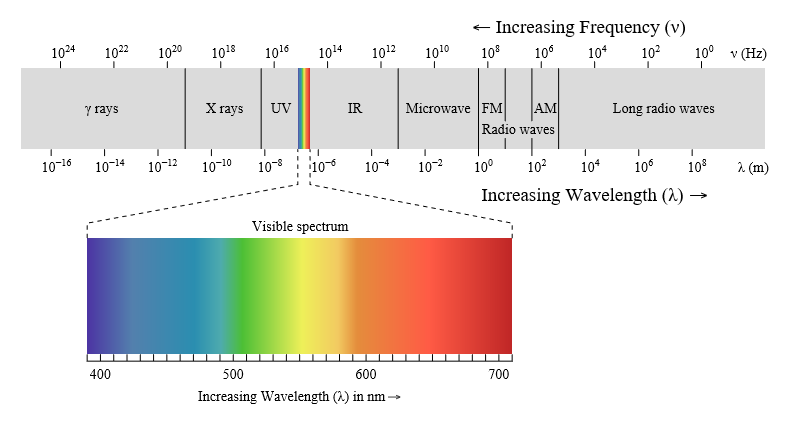
\includegraphics[width=\textwidth]{Includes/1-electromagnetic-spectrum.png}
        \caption{Electromagnetic spectrum}
        \label{fig:1-electromagnetic-spectrum}
    \end{figure}

    In the visual spectrum, usually reflected light is the measured. 
    In the Infrared spectrum (IR), light emitted from a certain wavelength is measured.
    This is because all bodies have a temperature above absolute zero, and this temperature is detectable as radiation.
    IR spectrum goes from 1400 nm wavelength to 1 mm and are further subdivided due to the width of the spectrum:

    \begin{itemize}
        \item  Short-wave infrared (SWIR): 1,4 to 3,0 µm
        \item  Medium-wave infrared (MWIR): 3,0 µm to 8 µm
        \item Long-wave infrared (LWIR): 8 to 15 µm
        \item Far-infrared (FIR): 15 µm to 1 mm
    \end{itemize}
    
    Like in the visual spectrum, TIR information is obtained in a purely passive way.
    Thermal infrared detectors called bolometers are mostly used on drones or ground stations due to their small volume, weight, and energy consumption. 
    They offer a low accuracy in relative and absolute temperature measurement and are relatively inert, leading to a low ground resolution for moving systems (drones) but worthwhile for aircrafts with small payloads.     
    More complex systems are generally cooled. Therefore, they offer the possibility of highly accurate relative and absolute temperature measurements.
    In contrast to bolometers, they are significantly larger and require more energy, making them unsuitable for use on drones.
    These types of detectors are used on all common TIR satellite systems.

    \subsection{Land surface temperature}

        Land Surface Temperature (LST) is the radiative temperature of the land surface. It is derived from previously mentioned thermal infrared radiation that the Earth’s surface emits.
        LST is essentially a measure of how hot Earth's surface would feel to the touch in a particular location.
        It is one of the key parameters that affect surface energy balance, regional climates, heat fluxes, and energy exchanges.
        When taking Earth’s temperature, we’re interested in thermal infrared (TIR) specifically, which has a wavelength of 3 to 14 µm (both MWIR and LWIR), corresponding to black body temperatures of between -60°C and 700 °C, according to plancks equation:
        
        \begin{equation}
            B_{\lambda}(T) = \frac{C_1}{\lambda^5 \left[ \exp\left(\frac{C_2}{\lambda T}\right) - 1\right]},
        \end{equation}
        
        Where $B_{\lambda}(T)$ is the spectral radiance, $C_1$ and $C_2$ are physical constants, and $\lambda$ is the wavelength of the radiation. 
        For this reason TIR wavelengths are of particular interest for this work.

        Accurate LST retrieval from TIR data depends on atmospheric effects, sensor parameters, i.e., spectral range and viewing angle, and surface parameters such as emissivity and geometry.
        Since emissivity and atmospheric effects are two fundamental factors to derive LST from thermal data, many researchers have proposed different approaches for LST retrieval considering these factors.
        These algorithms are named considering the number of TIR bands used. For instance, single-channel or mono-window algorithms use one TIR band. However, split window or multi-channel methods include more than one TIR band.
        Some examples of these methods are Radiative Transfer Equation (RTE) \cite{becker90}, Single Channel Algorithm (SCA) \cite{sca2009}, and Mono Window Algorithm (MWA) \cite{mwa2001}.
        As this work is focused on improving the resolution of the mapped radiances and not on the LST retrieval, the reader is referred to \cite{LI201314} for a more detailed review.

    \subsection{Quality dimensions of remote sensing data}

    Remote sensing data can be characterized by four quality dimensions, as stated in \cite{HORNING20082986}:

    \begin{itemize}
        \item Spatial resolution: This is often simply referred to as resolution and is the size of a pixel in ground dimensions. 
        In most cases an image's resolution is labeled with a single number, such as 30 m, which represents the length of a side of a square pixel if it were projected onto the Earth's surface.
        If the pixel were rectangular, then the length and width of the pixel would be provided.
        \item Spectral characteristics: This includes bandwidth, band placement, and the number of bands.
        Spectral bandwidth, or spectral resolution as it is often called, refers to the range of wavelengths that are detected in a particular image band.
        This is effectively a measure of how precisely an image band measures a portion of the EMS.
        Band placement defines the portion of the EMS that is used for a particular image band.
        For example, one band might detect blue wavelengths and another band might detect thermal wavelengths along the EMS.
        The properties of the features one is interested in sensing indicate which bands are important.
        The last spectral variable is the number of bands. The more bands that are available the more precisely spectral properties of a feature can be measured.
        \item Acquisition dynamics: This has two components. The first is the minimum time a particular feature can be recorded twice, often called the repeat frequency or temporal resolution.
        Some sensors with a very wide field of view can acquire multiple images of the same area in the same day whereas some sensors have a repeat frequency of several weeks.
        The other component is the timing of the acquisitions. 
        Dynamic features such as deciduous forests and events such as flooding often have an optimum time for which they should be imaged.
        For example, the identification of deciduous vegetation is aided by acquiring imagery during leaf-on and during leaf-off periods.
        \item Sensitivity of the sensor: This is defined by the dynamic range of the sensor as well as the range of digital numbers that can be used to represent the pixel values.
        Sensors have lower limits below which a signal is not registered and upper limits above which the sensor saturates and is unable to measure increases in radiance.
        The detail that can be measured between these extremes is determined by the range between the minimum and maximum digital numbers permitted for a particular data type.
        This potential range of values is often referred to as quantization or radiometric resolution.
    \end{itemize}
    
    
    

\section{Motivation}

Land Surface Temperature (LST) images at a high temporal resolution are of prime importance to efficiently 

Advancements in satellite technology, particularly in thermal infrared sensing, have emerged as a promising solution to monitor physical processes related to climate change such as water stress, evapotranspiration, wildfires or urban.
Unlike ground-based methods, satellites can continuously monitor vast tracts of land regardless of smoke or geographical barriers, providing critical real-time data that can significantly enhance early detection and response efforts. 
However, while current satellite systems offer extensive spatial coverage and consistent data collection, they are not without limitations. 
In particular, in the quality dimension of spatial and temporal resolution

Throughout this section, the main applications that OroraTech is working on are presented, as well as the thermal data products requirements that the literature has identified as vital for their development.
The trade-off between spatial and temporal resolution that the current available products will be further discussed, which is the main driver for super resolution.
    

    \subsection{Wildfire Monitoring}

    Forest fires can be natural or man-made phenomena that occurred in natural ecosystems and usually, they spread uncontrollably.
    The have increased steadily worldwide over the past decade, and according to the UN Environment Programme (UNEP), this trend will continue, with a potential 50\% increase in forest fires by the end of the century \cite{UNEP2021Wildfire}. 
    The escalating frequency and intensity of wildfires across the globe have prompted a reassessment of our current monitoring systems and methodologies. Traditional ground and aerial surveillance methods are increasingly proving inadequate in the face of rapidly spreading, unpredictable fires, particularly those obscured by smoke and difficult terrain. This inadequacy hinders effective firefighting efforts and exacerbates the environmental, economic, and human toll of these disasters. 
    Luckily, in most cases, a layer of fume is not an obstacle for a satellite to detect a fire, as they rely on thermal infrared sensors that can measure radiance through the smoke.

    Prevention is the most effective way to fight wildfires, and early detection is key to achieving this goal. 
    With timely access to thermal data from space, we gain the tools to identify potential wildfires before they spread, minimizing damage and saving lives.
    Although satellite-based imagery is used by emergency response agencies to monitor large-scale wildfires that burn over extensive periods, the wait interval for a satellite overpass induces a considerable time delay, which prevents its application in time-sensitive fire detection scenarios, such as emergency evacuations, early detection or search-and-rescue operations \cite{lippitt2015time}. 
    OroraTech's looks to circumvent the overpass wait interval by launching a swarm of small satellite that have  been especially helpful for detecting newly born fires that started as a result of a bigger fire spreading, burning the material around its vicinity. The team develops its own sensors capable of providing up-to-date thermal data of the entire Earth every 30 minutes, starting from 2026.
    
    However, another parameter vital to measure fire risk, detect burn areas, and monitor vegetation recovery is the spatial resolution. The coarse spatial resolution that the smaller payloads these satellites provide does not enable the reliable detection of smaller fires. Additionally, higher spatial resolution is needed to detect better estimate the fire front, which is vital for the emergency response teams to plan their actions.
    Moreover, High resolution data has been used to validate characteristics of false positives in fire detection algorithms applied to low resolution scenes\cite{ijgi11120601}. 



    \subsection{Urban heat}

    Productivity losses due to heat currently cost an estimated \$100 billion annually only in the U.S alone.
    The U.K. experienced unprecedented temperatures too, temporarily knocking out services for giants like Google and Oracle and further affecting their clients.
    These are only a few examples of how businesses are affected by extreme temperatures in urban areas \cite{atlanticcouncil2021extreme}.  

    Public interest and concern about heat waves are steadily rising, especially in moderate climate areas such as North Europe. Heat waves are a major cause, specially in vulnerable population such as elderly people who are more prone to heat stress, pregnant individuals with difficulty adjusting to heat changes, outdoor workers who are exposed to extreme heat for prolonged periods and low-income neighborhoods with poor-quality buildings, between others \cite{Hsu2021Disproportionate}.   

    Urban heat refers to the phenomenon where urban areas experience higher temperatures than their more rural surroundings.
    This effect can be attributed to various factors such as building geometry, thermal properties of building materials, radiation properties of surfaces, and anthropogenic heat release from sources such as traffic and industry \cite{deilami2018urban}. 
    In particular,  the Urban Heat Island (UHI) phenomenon refers to the air temperature differences between urban areas and their surrounding rural regions, which is typically most pronounced during the evening and night hours. 

    Monitoring the UHI effect traditionally involves recording measurements from meteorological stations located in urban and rural areas throughout the region.
    However, an alternative method is to use thermal remote sensing, which allows for the monitoring of large areas without the need for multiple physical sensors placed throughout the city.
    Research suggests that a Ground Sampling Distance (GSD) of 50m to 100m is the most suitable spatial resolution for urban thermal environment studies \cite{mohamed2017land, sobrino2012impact, huang2013generating}. 
    This spatial resolution requirement can be met by missions such as Landsat \cite{USGS2023Landsat} and Terra \cite{terra_nasa}, which provide a high spatial resolution in the thermal infrared band.
    However, their insufficient revisit time severely limits the analysis of dynamic processes with a temporal resolution in the order of hours, such as the UHI. 

    Existing studies on the UHI effect have been limited by the low spatial resolution of the images used and the lack of satellite images available at different times of the day \cite{Zhu2021, Shi2019}. 
    In particular, researchers explicitly state their limitations \cite{Shi2019} due to the low frequency of revisits while studying the Park Cool Island (PCI) \cite{Yang2017} phenomenon. 
    The influence of vegetation cover on the urban heat island (UHI) phenomenon has been recognized as the foremost determinant \cite{deilami2018urban}, where parks have been found to exert a cooling impact.
    Figure \ref{fig:1-skopie-UHI} illustrates an example that demonstrates this influence. 
    Converting the low-resolution images coming from private constellations into high-resolution images through post-processing techniques could enable new frontiers in the study of urban heat. 

    \begin{figure}[H]
        \centering
        \begin{minipage}{0.5\textwidth}
            \centering
            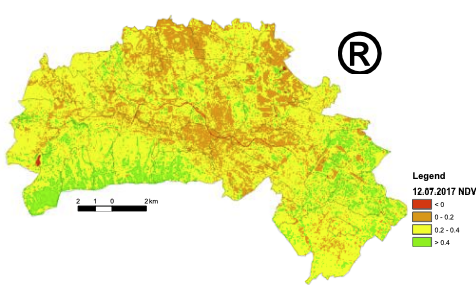
\includegraphics[width=\textwidth]{includes/1-skopje-NDVI.png}
            \label{fig:1-skopje-NDVI}
        \end{minipage}\hfill
        \begin{minipage}{0.5\textwidth}
            \centering
            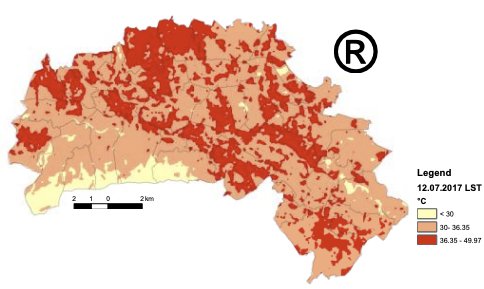
\includegraphics[width=\textwidth]{includes/1-skopje-LST.png}
            \label{fig:1-skopje-LST}
        \end{minipage}
        \caption{Normalized Difference Vegetation Index \cite{Rouse1973MonitoringVS} and LST measurements for the zone of Skopje, North Macedonia. Urban areas with a lower vegetation index tend to have a higher temperature than their rural counterparts. Source : \cite{skopje2018}.} 
        \label{fig:1-skopie-UHI}
    \end{figure}


    \subsection{The spatio-temporal trade off}

        Sensors typically trade spatial resolution for temporal resolution and, it has been difficult historically to maximize both.
        Sensors that have a high spatial resolution often cover a smaller area than a sensor with lower spatial resolution.
        With a smaller field of view, it takes longer to cover the same area, thus as spatial resolution increases, temporal resolution decreases.

        Essentially, it can be said that currently, the TIR data products that are used for developing LST data has either: 
        
        \begin{itemize}
            \item high temporal resolution (sub-daily images) but very low spatial resolution ( in the km range).
            \item High spatial resolution ( < 100 m) but low temporal resolution (several days up to weeks).
        \end{itemize}

        Unfortunately, the applications mentioned before have requirements in both spatial and temporal resolution. 
        The zone of interest, composed of sub-daily frequency and a GSD smaller than 100m, is not covered by any of the existing systems.
        Private missions, using smaller satellites, can leverage on constellations  to provide a higher temporal resolution.
        However, the spatial resolution is still limited by the payload mass and energy consumption constraints.
        This trade-off can be described by displaying the resolution of some of the LST/TIR data products available, as in Fig. \ref{fig:1-spatio-temporal-trade-off}. 

        \begin{figure}[H]
            \centering
            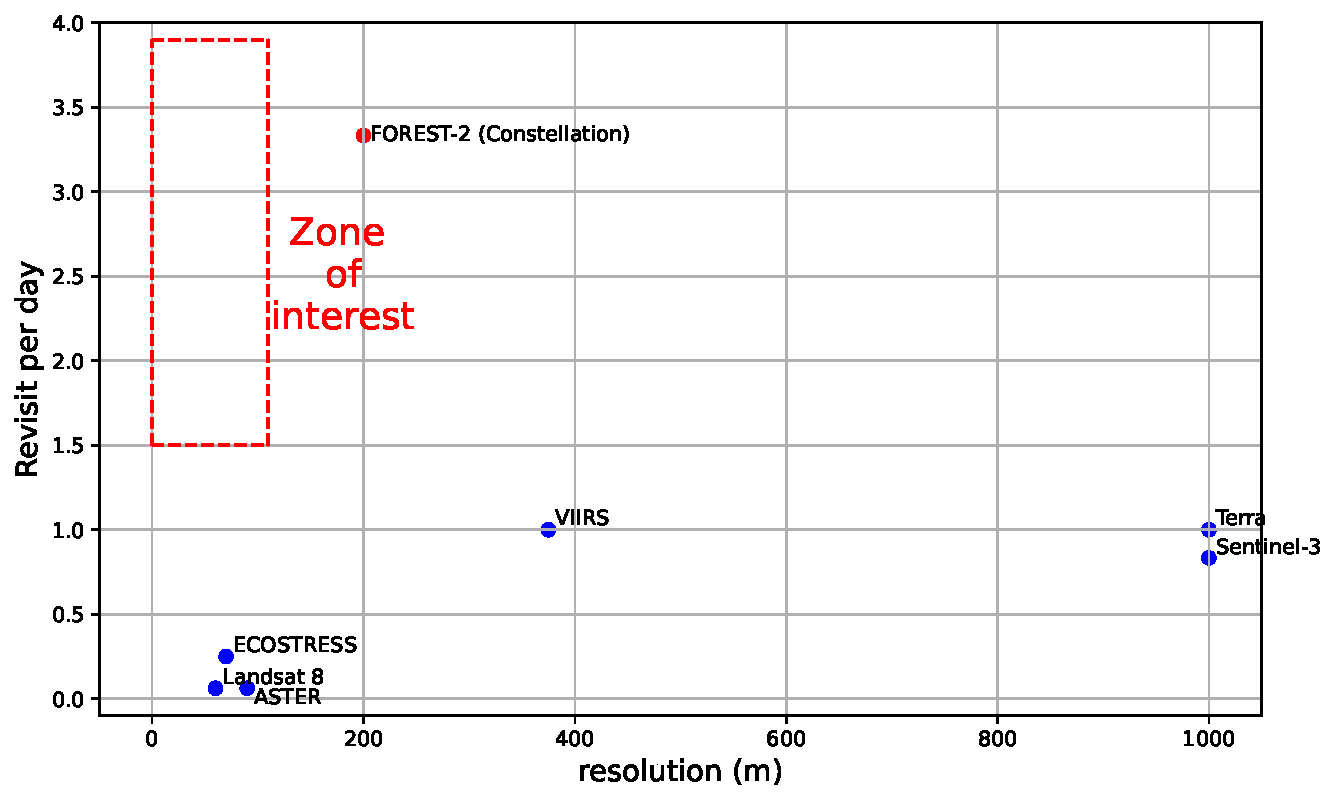
\includegraphics[width=\textwidth]{Includes/2-scatterplot-res-revisit.pdf}
            \caption{Scatter plot of the spatial and temporal resolution of some of the LST/TIR data products available.
                     The trade-off is evident, no mission can provide products in the zone of interest.
                     Constellations may help with temporal resolution, but the spatial resolution is still limited.}
            \label{fig:1-spatio-temporal-trade-off}
        \end{figure}

        This opens the question of whether it is possible to increase the spatial resolution of the data products available using a post-processing technique such as super resolution, without compromising the physical consistency of the scenes.
        The main techniques of super resolution and their most difficult challenges to apply them to LST/TIR data are described in the next section.

\newpage
\section{Super resolution} \label{sec:SR}

    Super resolution refers to an image processing process of recovering a corresponding high-resolution image from a low-resolution version of it, with applications that range from natural images \cite{zeyde2010single}, \cite{martin2001database} to satellite \cite{valsesia2021permutation} and medical imaging \cite{bashir2021comprehensive}. SR remains a challenging task in computer vision because it is considered an ill-posed problem: several HR images can generate exactly the same LR image. 

       \begin{figure}[h!]
            \centering
            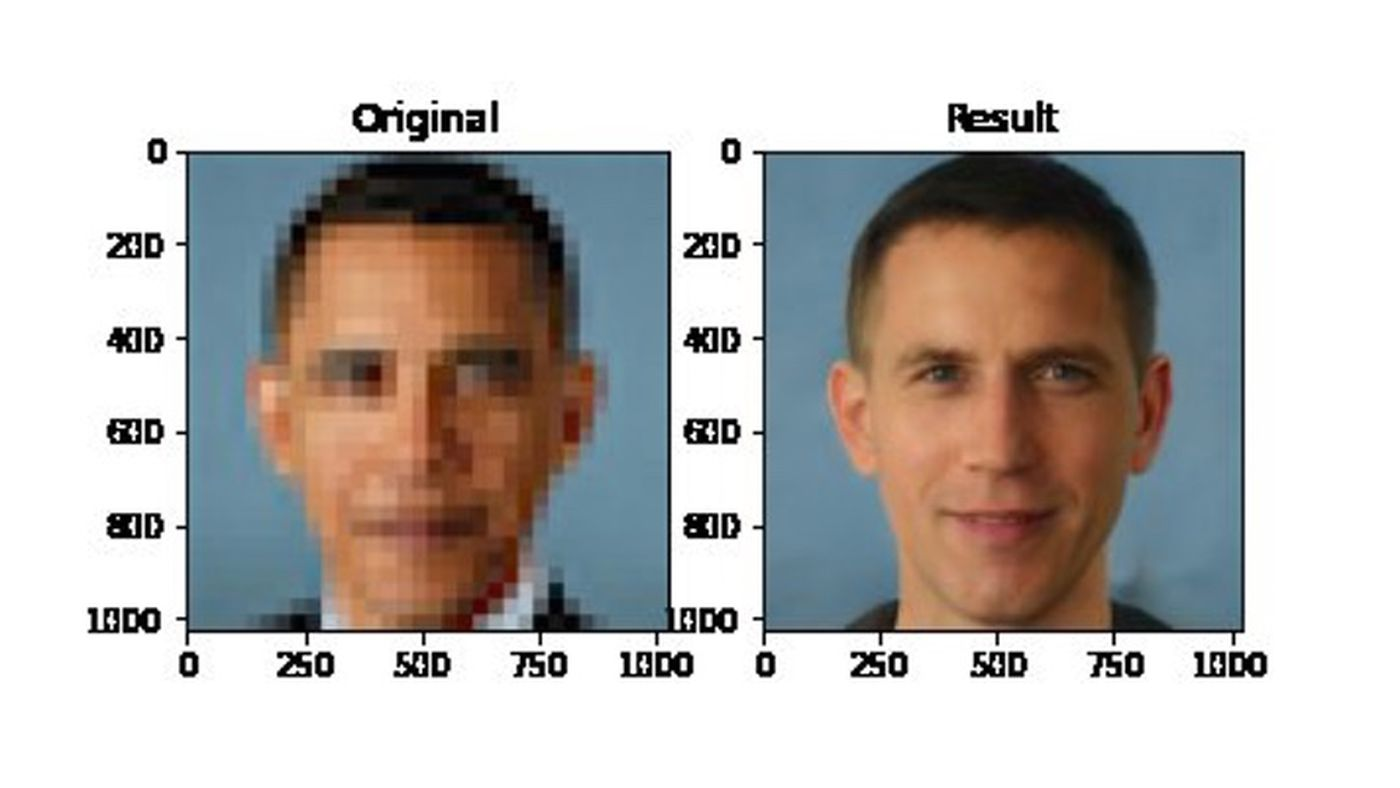
\includegraphics[scale=0.2]{Includes/2-SR-ill-posed.jpg}
            \caption{Example of super resolution as an ill posed problem. A blurry picture of Barack Obama can be generated from an HR image of another person.}
            \label{fig:2-SR-ill-posed}
        \end{figure}
    
    Depending on the different number of low-resolution inputs, image super resolution reconstruction can be divided into single-image or multi-image. ASDFAGDSGADFSGAFSFAD

    Traditional interpolation-based methods for upsampling images were the first type of algorithms used for super resolution. The most common techniques are nearest-neighbor, bilinear and bicubic interpolation. Nearest-neighbor interpolation is the most straightforward algorithm, as the interpolated value is based on its nearest pixel values.  While this method requires almost no calculations, the results are usually blocky because there are no interpolated smooth transitions.
    Bilinear and bicubic interpolation produces smoother transitions using linear or cubic interpolation in both axes. Bilinear interpolation needs a receptive fields of 2x2 and is usually faster, bicubic needs a receptive field of 4x4. THe latter is the most common baseline to understand the improvement of a super resolution network. 

    

\begin{itemize}
    \item what is super resolution?
    \item Interpolation based vs reconstruction-based vs learning-based
\end{itemize}

    \subsection{single-Image Super Resolution}

        In a typical SISR framework, the LR image $I^{LR}$ is modeled as follows:
    
        \begin{equation}
            I^{LR} = ( I^{HR} \ast k) \downarrow_s + \ n
        \end{equation}
    
        Where $I^{HR} \ast k$ is the convolution between a blurring kernel $k$ and the unknown  HR image  $I^{HR}$, $\downarrow_s$ is the downsampling operator with scaling factor $s$ and $n$ is a noise term. Super resolution objective is to solve this equation and obtain $I^{HR}$ which as stated before, is an extremely ill-posed problem. Super resolution was first proposed in the 1960s, while the first use of multiple images dates of 1989. Machine learning was used for the first time in 2000. Deep learning appears as a branch of machine learning, emphasizing the use of multi-layer neural network cascade for feature exctraction and representation. The rise of the technology wave around 2010 changed the way of solving problems in different branches. Instead of piecing together individual functional modules to form a system, the focus is to optimize parameters by global training after the whole system is designed, what is called end-to-end training. 
        \subsubsection{SR Resnet}
    \subsection{Multi-Image Super Resolution}

        Multi-Image Super-Resolution (MISR) is the task of yielding HR images by fusing multiple LR observations of the same scene, which allows the achievement of higher reconstruction accuracy than relying on only one image. The development of this approach progressed at a slower pace due to the extesive pre-processing requirements imposed on the input, as this algorithms have a high sensibility to the input variability and their proper co-registration.  

        When the input images are of the same nature, but taken at different points in the temporal dimension, the problem is often called multi-image super resolution. On the other hand, when the images are taken at the same time but they come from different sensors and show different spectral bands, it is called multi-spectral super resolution, which will be further discussed. 

        In 2019, the European Space Agency (ESA) organized an SR challenge  \cite{märtens2019superresolution} based on real-world scenes acquired by the PROBA-V satellite, each of which contains an HR image (100m GSD) coupled with at least nine LR images that are not perfectly co-registered and they may be taken months apart. This challenge, with a not synthetically generated HR-LR image pairs, fostered a new generation of model architectures that are able to fuse the multiple LR images to create better reconstructions.

        \begin{figure}[h!]
            \centering
            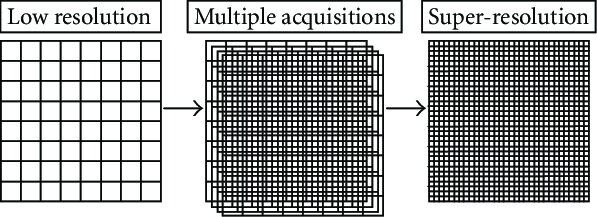
\includegraphics[scale=1.5]{Includes/2-MISR.jpeg}
            \caption{Multi-image super resolution algorithms combine multiple low-resolution image acquisitions into a high-resolution image. Source: \cite{MISR2007}}
            \label{fig:2-SR-ill-posed}
        \end{figure}
        
        \subsubsection{Multi-spectral super resolution}

        Also Referred to as "hyper-spectral super resolution" in the literature, The term "Multi-Spectral" emphasizes the use of multiple spectral bands, in contrast with the multi-image approach detailed previously. While the concept bears similarities to MISR, the key distinction lies in MSSR's use of a single scene captured with different spectral bands, as opposed to multiple images, to reconstruct a superior, super-resolved image.

        In the context of MSSR, each spectral band, corresponding to a specific wavelenght range, provides unique information about the observed scene. Some of the spectral bands yield better resolution because of their physical properties and the costs related to their sensors. Using this higher resolution bands to increase the detail in the lower bands seems like a resaonable approach.

        Traditional pan-sharpening algorithms could be considered as deterministic MSSR  algorithms. It is usually used to increase the resolution of a multi-spectral RGB image using the panchromatic band. The overlap between the wavelengths of both wavelength ranges makes this algorithm straightforward. However, it is ill-suited for Thermal Infrared (TIR) data due to the disjointed spectral domains of the visible and TIR bands. In \cite{myself2023}, A deep learning is trained assuming the presence of common information between low-resolution LWIR images and their higher resolution RGB counterparts, with the objective of creating a super-resolved product in the LWIR band by an effective fusion. This improved image retains the essential thermal information, while simultaneously incorporated enhanced spatial resolution details captured from the visible bands. 

        \subsubsection{Importance of interframe correlation}
        \subsubsection{RAMS}
    \subsection{Data requirements}
        \subsubsection{Super Resolution as a supervised problem}      

        SR is a supervised problem, the super resolved image is compared to the HR ground truth and the differences between them drives the gradients of the neural network to minimize the loss.
        \subsubsection{Applying a basic degradation model}

        
        \subsubsection{The domain gap problem}

    \subsection{Blind image Super Resolution}
    
        Blind SR for unknown degradation is proposed to bridge the domain gap present in the synthetic datasets generated using bicubic downsampling.
    

        \begin{figure}[h!]
            \centering
            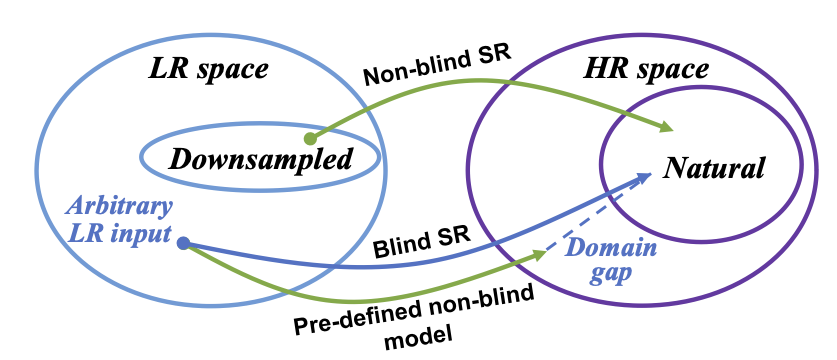
\includegraphics[scale=0.45]{Includes/2-DomainGap.png}
            \caption{Domain interpretation of differences between non-blind and blind SR. Source: \cite{liu2021blind}}
            \label{fig:2-SR-ill-posed}
        \end{figure}

        Nevertheless, real-world degradations are usually too complex to be modelled with an explicit combination of multiple degradation types, as shown in Fig.3(c). Therefore, implicit modelling attempts to circumvent the explicit modelling function. Instead, it defines the degradation process f implicitly through data distribution, and all the existing approaches with implicit modelling require an external dataset for training. Typically, these methods utilize data distribution learning with Generative Adversarial Network (GAN) [16] to grasp the implicit degradation model possessed within training dataset, like CinCGAN [8].

\clearpage
\section{Methodology} \label{sec:methodology}

Throughout this section, the selected architectures for the blind super resolution task will be explained in-depth, along with the rationale behind their choice. Additionally, all the metrics and losses used during training and experimentation will be introduced. 
Moreover, a process to create a baseline dataset to assess the performance of the selected architecture is explained in detail. 


\subsection{Models architecture}

\subsubsection{Probabilistic degradation model}

    The probabilistic degradation model architecture, introduced in \cite{luo2022learning}, is classified among implicit modeling methods for blind super resolution.
    Typically, models in this category aim to learn the degradation process adaptively through deterministic models. Nevertheless, specific degradations in practical scenarios show stochastic behavior and do not strictly correlate with the image's content. Such methods may struggle to capture these unpredictable elements and the content-independent aspects of degradation, potentially constraining the performance of the subsequent SR model. In this particular architecture, the degradation \(D\) is assumed as a random variable, and two networks seek to learn its distribution by mapping two random variables $z_k$ and $z_n$ to \(D\). 

    Contrary to previous models that use deep learning to directly transform an HR image into an LR one, this strategy employs two networks to generate a blurring kernel and additive noise, following Eq. \ref{eq:2-degradation-equation}. This constraint imposes limitations on how the degradation affects the images, thus making its integration with an SR model easier and allowing efficient end-to-end training. Additionally, it provides actionable insight into understanding the unknown degradation process.
    The stochastic nature of the model allows the production of a wider variety of degradations, thereby allowing the creation of diverse HR-LR pairs. This diversity covers the possible degradations in test LR images and prevents the SR model from overfitting to specific scenarios.

    
    The degradation is parametrized using two random variables, the blur kernel $k$ and random noise $n$, by formulating the degradation process as the linear function from Eq. \ref{eq:2-degradation-equation}.
    The equation can be divided into two linear steps \cite{zhu2020unpaired}: 

    \begin{equation}
        \begin{aligned}
                I^{\text{LR}}_{\text{clean}} &= (I^{\text{HR}} * k) \downarrow_s \\
                I^{\text{LR}} &= I^{\text{LR}}_{\text{clean}} + n
        \end{aligned}
    \end{equation}
    
    In most cases, the two steps are mutually independent, as the blur kernels are mainly dependent on the properties of the camera lens, and the noises are primarily related to the properties of sensors. 
    Thus, the distribution of the degradation process can be represented as the product of the distribution of $k$ and $n$, which can be modeled by learning the mapping from random variable $z_k$ and $z_n$ to $k$ and $n$, respectively.


    \begin{equation}
        p_{D}(D) = p_{k,n}(k, n) = p_{k}(k)p_{n}(n).
    \end{equation}

    To model the distribution of the blur kernel k, a random variable $z_k$, which is subject to a multi-dimensional normal distribution, is defined. 
    Then, a generative module is used to learn the mapping from $z_k$ to $k$. 

    \begin{equation}
        k = \text{net}K(z_k), \quad z_k \sim \mathcal{N}(0,1),
    \end{equation}

    The spatially variant blur kernel is considered first. This implies that the blur kernel for each pixel of the image is different. In that case, the shapes of $z_k$ and $k$ are:

    \begin{equation}
        z_k \in \mathbb{R}^{f_k \times H \times W}, \quad k \in \mathbb{R}^{(k \times k) \times H \times W},
    \end{equation}

    Where $f_k$ is the dimension of the normal distribution $z_k$ and $k$ is the size of the blur kernel. $H$ and $W$ represent the height and width of the image, respectively.
    Generally, the sizes of the convolutional weights are set as 3 × 3, which indicates that the learned blur kernels of neighboring pixels are spatially correlated.
    If the spatial size of all convolutional weights is set as 1 × 1, the blur kernel could be approximated by a spatially invariant one, which is a particular case of the spatially variant blur kernel with $H = W = 1$.
    This approximation simplifies the dimensions of the problem drastically and is an appropriate assumption if the crops used for training the model are small.
    A softmax layer is added at the end of the network to guarantee that the sum of all elements of $k$ equals to one.
    
    
    To model the distribution of the noise $n$, a  generative module can also be used:

    \begin{equation}
        n = \text{net}N(z_n), \quad z_n \sim \mathcal{N}(0,1),
    \end{equation}

    \begin{equation}
        z_n \in \mathbb{R}^{f_n \times H \times W}, \quad n \in \mathbb{R}^{C \times H \times W },
    \end{equation}

    Where the height, width, and number of channels of the image are noted as $H$, $W$, and $C$, respectively. 
    In this work, $C$ is always set to 1.

    In other methods \cite{plotz2017benchmarking}, the noise is modeled as a combination of shot and read noise. 
    It can be approximated as a heteroscedastic Gaussian distribution, which is dependent on the content of the image:

    \begin{equation}
        n \sim \mathcal{N}(0, \sigma_{\text{read}} + \sigma_{\text{shot}} \cdot I^{\text{LR}}_{\text{clean}}),
    \end{equation}

    This indicates that the noise is also related to the image content, and the distribution of $n$ should be expressed as:


    \begin{equation}
        n = \text{net}N(z_n,I^{\text{LR}}_{\text{clean}}), \quad z_n \sim \mathcal{N}(0,1),
    \end{equation}

    \begin{figure}[h!]
        \centering
        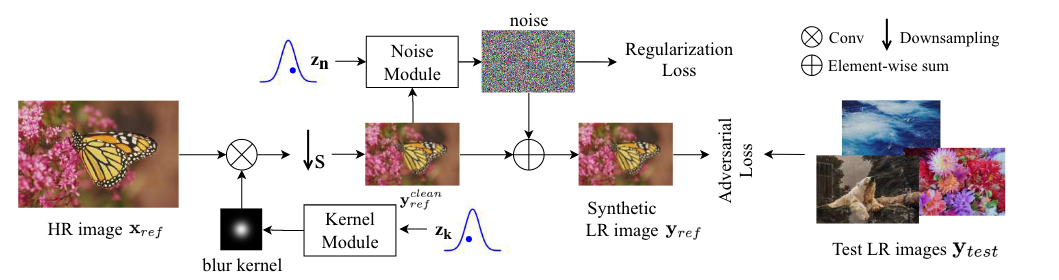
\includegraphics[width=\textwidth]{Includes/3-probabilistic-degradation-model.png}
        \caption{Schematic of the probabilistic degradation module.
                The discriminator is left out for a more intuitive description (source: \cite{luo2022learning}).}
        \label{fig:3-probabilistic-degradation-model}
    \end{figure}

    The probabilistic degradation model is optimized via adversarial training, which encourages the output of the generator to be similar to the test LR images \cite{bulat2018learn}.
    To avoid overly noisy images, a constraint to the noise level is added to the loss function via a regularization term. 
    A multiplication constant is also added to balance the magnitude of the two terms.

    \begin{equation}
        \mathcal{L}_{\text{total}} = \mathcal{L}_{\text{adversarial}} + 100 \cdot \|n\|_2^2.
    \end{equation}

    This approach formulates the degradation process as a linear function, and the learned degradations can only impose a limited influence on the image content.
    This way, it decouples the degradations with image content better and it places the focus on learning the degradations.
    This limitation imposed on the generator eliminates the need for guidance using a bicubically downscaled version of the HR image, as opposed to \cite{wei2020unsupervised} or \cite{bulat2018learn}.

    \begin{figure}[H]
        \centering
        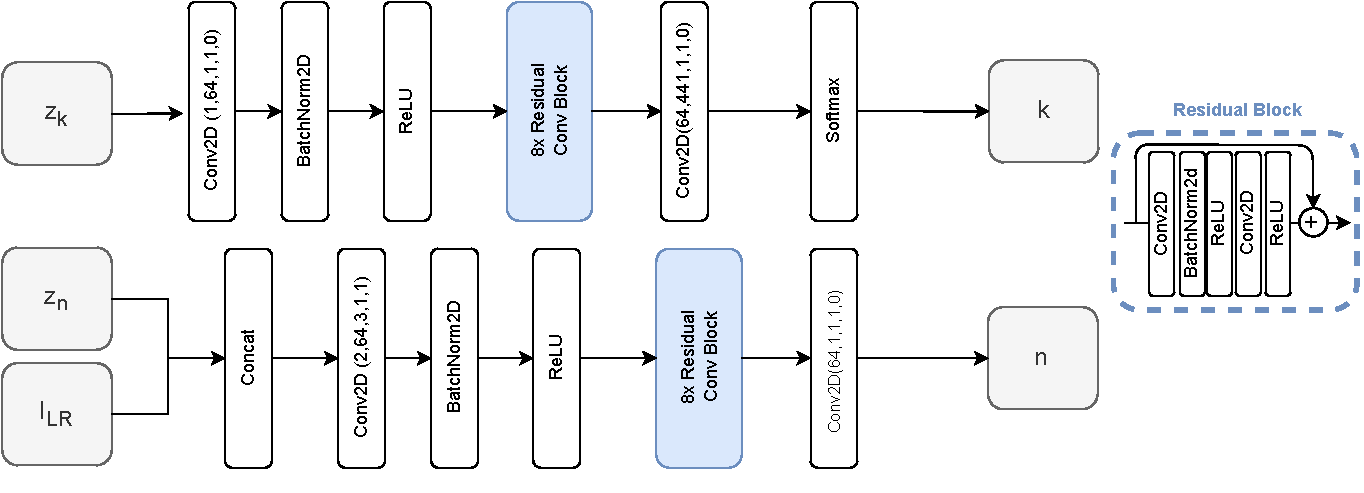
\includegraphics[width=\textwidth]{Includes/3-slim-gen-module.pdf}
        \caption{Schematic of the generative networks used in the kernel and noise module of the probabilistic degradation model.
        The parameters of the convolutional layers represent input channels, output channels, kernel size, stride, and padding, respectively.
        The residual blocks use the same kernel size as the convolutional layers of each module.}
        \label{fig:3-slim-gen-module}
    \end{figure}

    To discriminate the generated images from the test images, a PatchGAN discriminator is used \cite{isola2018imagetoimage}. This architecture assesses the structure of local image patches, allowing it to focus on high-frequency details of the image. This is particularly useful in the context of this approach, where the generated images are expected to share a lot of information in the low frequencies of the domain, and the differences with the real LR images are expected to be in the high frequencies. The architecture of the discriminator is shown in Fig. \ref{fig:3-slim-patchgan-module}.
    The network seeks to classify patches of an image as real or fake. The size of the patches depends mainly on the number of strided convolutional layers that are employed. The discriminator outputs a matrix of values, where each value represents the probability that the corresponding patch is real. The final output is obtained by averaging the values in the matrix.

    \begin{figure}[H]
        \centering
        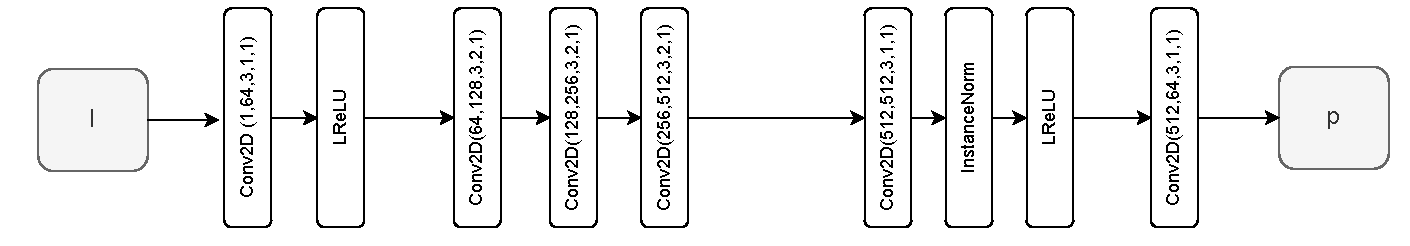
\includegraphics[width=\textwidth]{Includes/3-slim_patchGAN_architecture.pdf}
        \caption{Diagram of the PatchGAN discriminator.
                 The parameters of the convolutional layers represent input channels, output channels, kernel size, stride, and padding, respectively. }
        \label{fig:3-slim-patchgan-module}
    \end{figure}

    
    The constrained nature of the probabilistic degradation model allows the possibility to train it simultaneously with a super resolution algorithm, as described in Fig. \ref{fig:3-GAN-degradation-model}.      
    This way, it can be integrated with any SR model to form a unified framework for blind SR that can be trained in an end-to-end fashion, allowing faster iterations.
    Other methods \cite{fritsche2019frequency,wei2020unsupervised} require that the training of the degradation model and the SR model be in separate phases. First they train a degradation model and then use the trained degradation model to generate pairs and train the SR model.
    This two-step training method is time-consuming but necessary because the highly nonlinear degradation models used will produce undesirable results at the beginning of the training, which may mislead the optimization of the SR model.

    \begin{figure}[H]
        \centering
        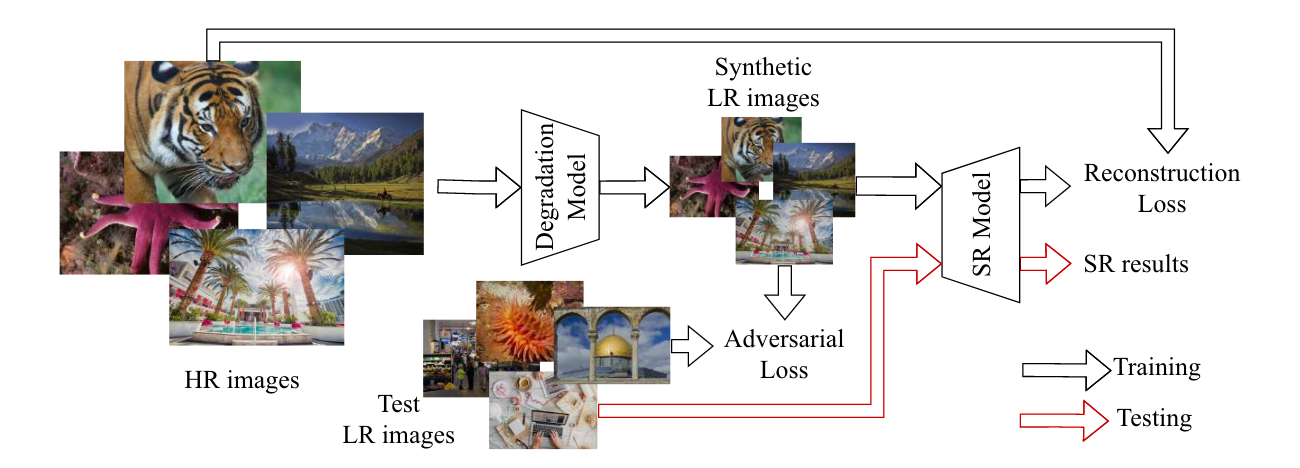
\includegraphics[width=\textwidth]{Includes/3-GAN-degradation-model.png}
        \caption{The probabilistic degradation model is used to encourage the degradation model to produce images in the same domain as the test LR images.
                After training, the SR model is directly used to process the inputs (source \cite{luo2022learning}).}
        \label{fig:3-GAN-degradation-model}
    \end{figure}

    The probabilistic degradation model constitutes a flexible framework for blind super resolution. 
    The only data requirement is a big enough unpaired dataset of LR and HR images and an optional smaller paired dataset for validation and early stopping of the model training.
    The most significant limitation of this approach is the one that implicit modeling methods have: the HR images (source domain) and the LR images (target domain) must be well defined for the model to generalize to a domain that is not in the datasets. 
    Using this framework for general images is difficult due to the variety of cameras, sensors, and compression algorithms that play a part in image distribution. Nevertheless, in the context of this study, the remote sensing images are characterized by a well-defined degradation process that remains relatively stable over time.


\subsubsection{SRResNet}

    
    The SRResNet architecture is used to perform the super resolution task. This network has been used extensively in the literature and has proven to be a good baseline for SR. It can also be easily extended for multi-spectral super resolution, as in \cite{myself2023}. It uses a residual network architecture in a post-upsampling framework based on sub-pixel convolution layers.
    
    Introduced in 2017 \cite{ledig2017photorealistic}, SRResnet is the generator in the SRGAN architecture, which is a GAN-based super resolution method. The purpose of the GAN is to drive the reconstruction process towards the natural image manifold, producing more visually convincing solutions. Additionally, a perceptual loss based on activation layers of a pre-trained VGG network \cite{simonyan2015deep} is incorporated into the pixel loss training objective. As this work focuses on having super-resolved images with high physical consistency and not on the perceptual superiority of the images, these two components are left out,  keeping only the generator and the pixel loss. The architecture, with slight modifications, is detailed in Fig. \ref{fig:3-resnet-architecture}.

    First, features are extracted from the input using a convolutional layer with 64 filters and a kernel size of 3, plus a ParametricReLU activation function.
    Before going through the core of the network, the feature map is reduced by half using a 1x1 convolutional layer.
    The core of the network is composed of five residual blocks, consisting of two convolutional layers, followed by batch-normalization layers and ParametricReLU activation functions. 
    The convolutional layers have 3x3 kernels and sixty-four feature maps. 
    Two trained sub-pixel convolution layers are used to increase the resolution of the input image.

    \begin{figure}[H]
        \centering
        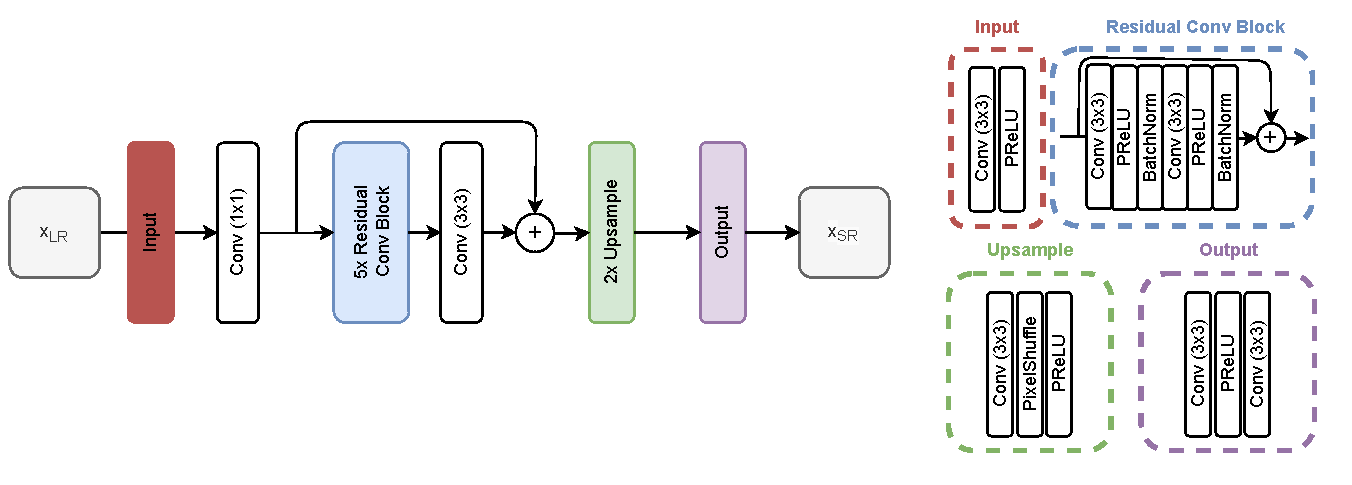
\includegraphics[width=1\textwidth]{Includes/3-srresnet-architecture.pdf}
        \caption{ Modified SRResNet architecture. $X_{LR}$ represents the LR input image, $X_{SR}$ the super-resolved image, which is then compared to the ground truth $X_{HR}$.}
        \label{fig:3-resnet-architecture}
     \end{figure}
    
    \subsection{Baseline degradation model} \label{subsec:baseline_degradation_model}

        As stated in \ref{subsec:domaingap}, early super-resolution methods commonly generated paired HR-LR samples using predefined degradation techniques, with bicubic downsampling being the most used setting \cite{zhang2018residual}.
        This kind of synthetic data, while easy to obtain, often results in a domain gap problem, where the data used for training and assessing the model do not come from the same distribution as the real data. This gap usually leads to decreased performance when the models are deployed in production environments.
        
        A possible solution is to synthesize samples with a stochastic degradation model, which includes a set of multiple blurring kernels and several random noise configurations that convert scenes from an HR mission into LR versions.
        The larger degradation space grants these models better generalization capabilities and lets experts be part of the kernel definition process based on prior knowledge of the degradation process.
        However, the variety of predefined degradations is limited and still fails in most applications. A degradation model like this one will be used to generate a baseline dataset for this work.
        

        \subsubsection{Blurring kernel}

        In the literature, the kernel of the degradation process is usually modeled as a fixed isotropic Gaussian kernel, with a parameter $\sigma$ that depends on the scale factor of the super resolution process.
        To provide more variability to each dataset pair, the parameters of the blurring kernel that determine its width in both axes, $\sigma_x$ and $\sigma_y$, are sampled from a normal distribution with a determined mean and standard deviation. Fig. \ref{fig:4-degradation_kernels} shows some examples of kernels generated using this method; in the upper row, both distributions have a similar mean and variance, resulting in approximate isotropic kernels. In the lower row, the mean of the x-axis is much higher than the mean of the y-axis, resulting in anisotropic kernels. The effects of these kernels on the HR-LR generation are shown in Fig. \ref{fig:4-degradation-kernel-examples}.



        \begin{figure}[H]
                \centering
                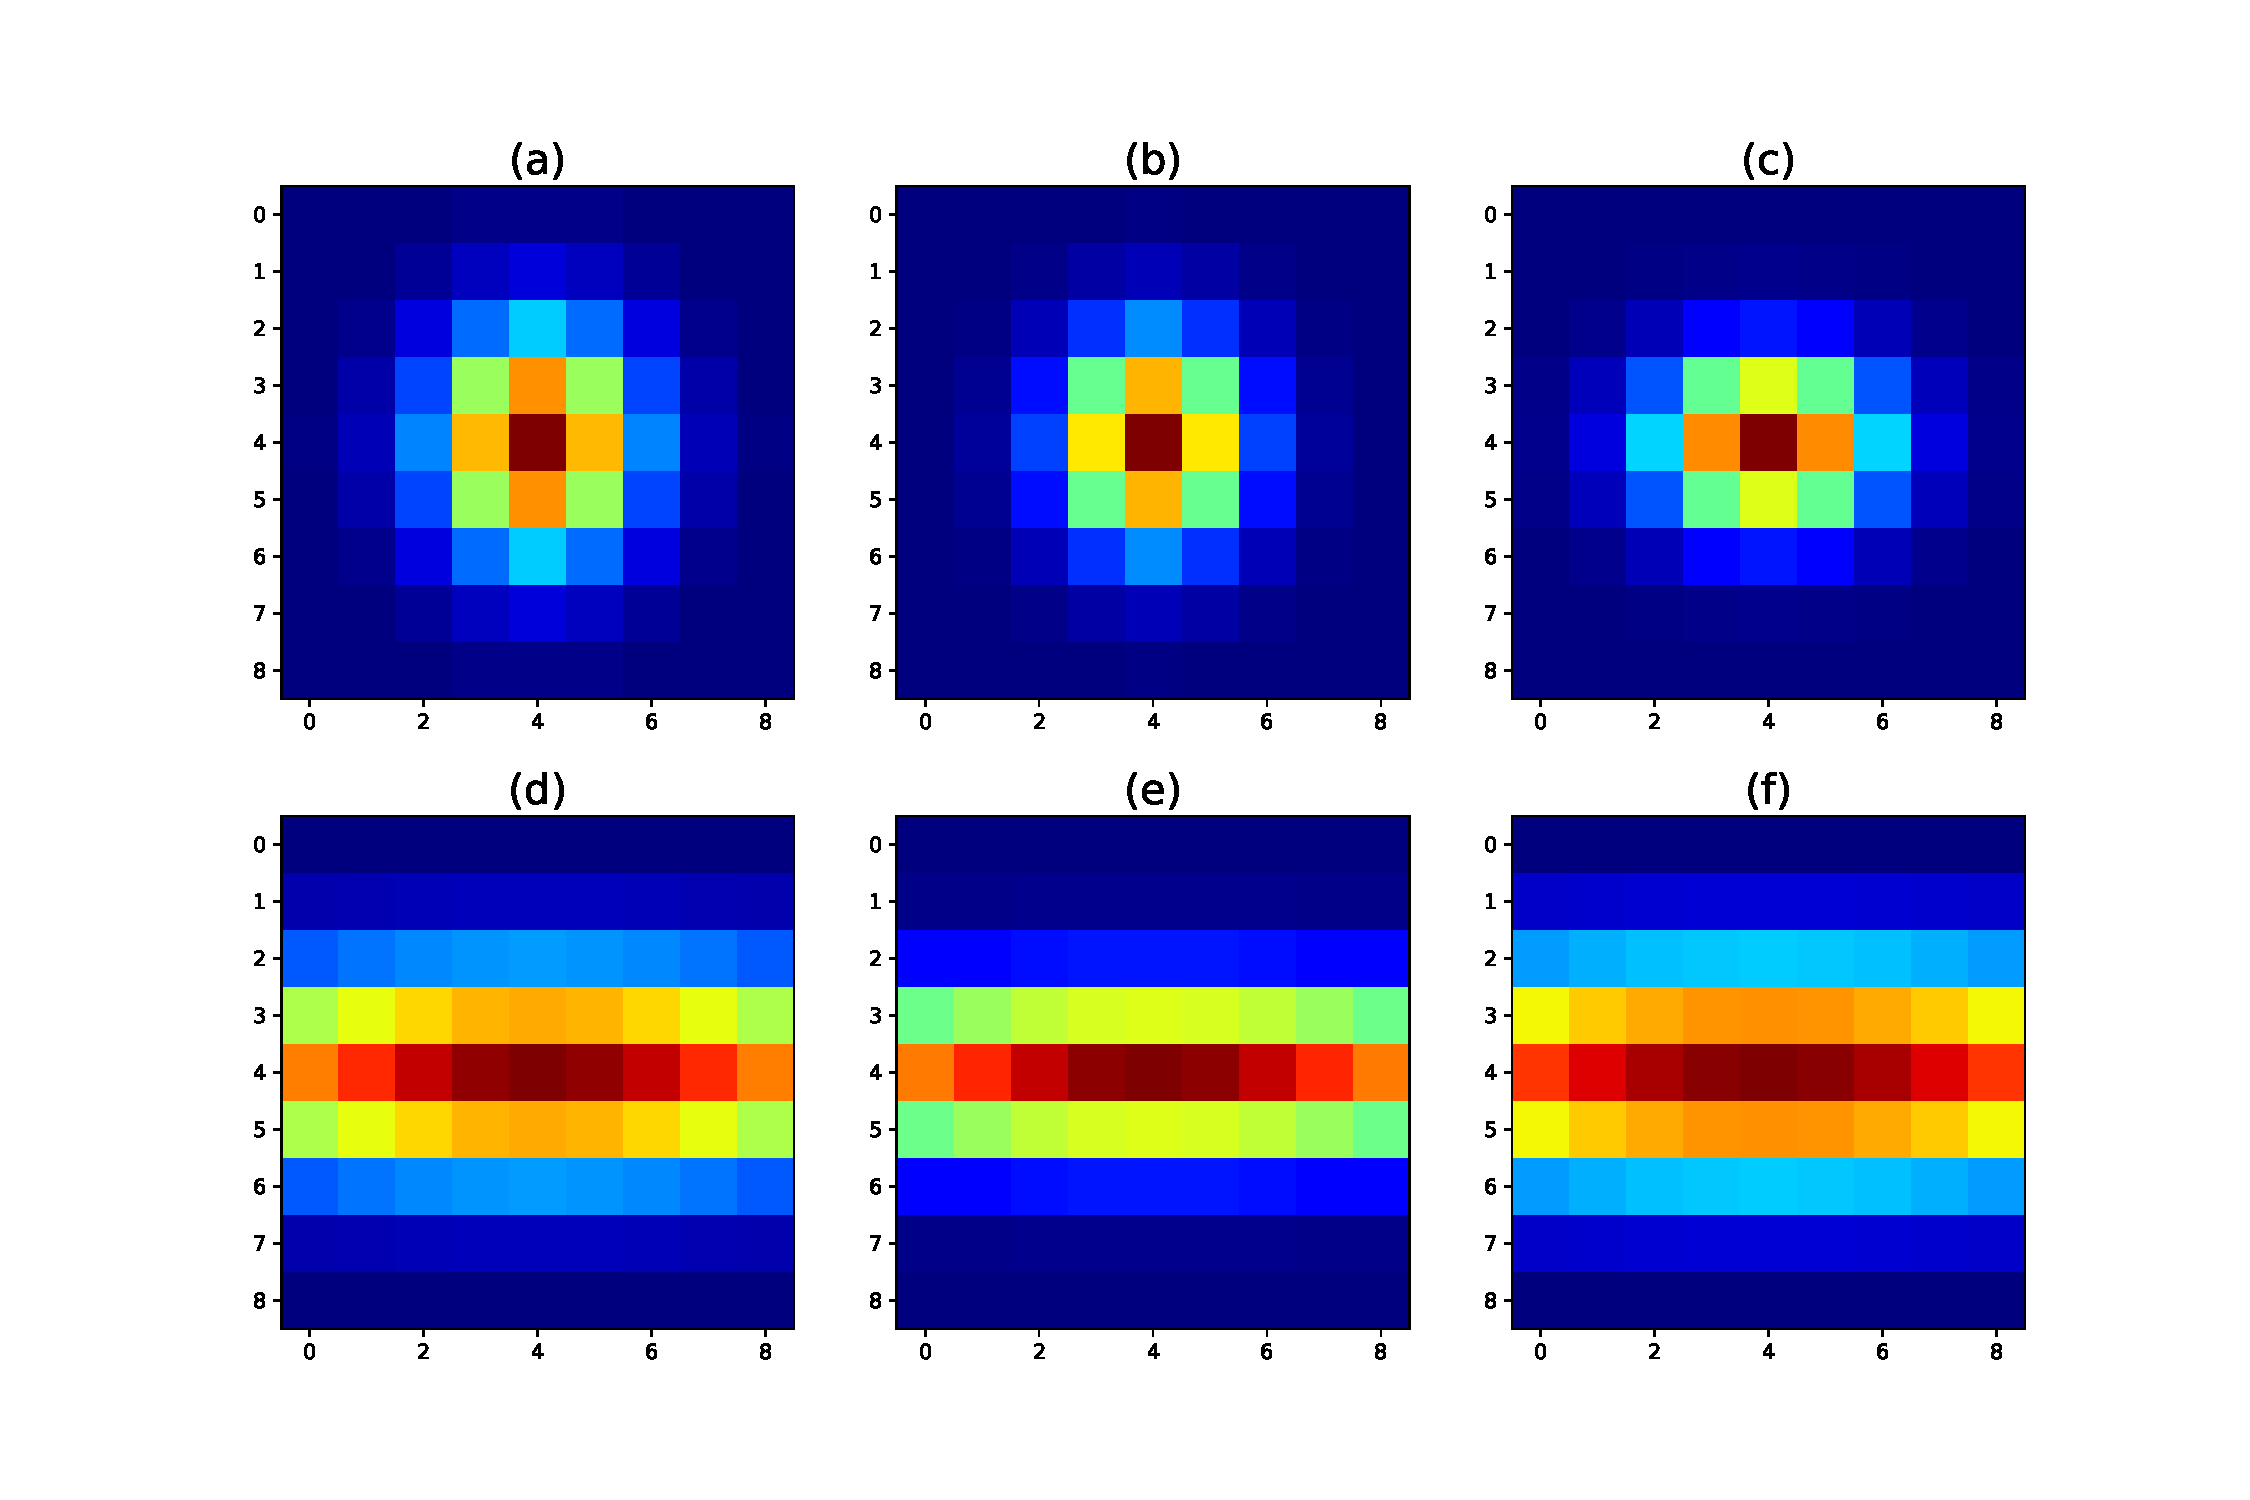
\includegraphics[width=\linewidth]{Includes/4-degradation_kernels.pdf}
                \caption{Example of kernels used in a stochastic degradation model. (a),(b) and (c) are generated using a symmetric variance on the x and y-axis. (d) (e) and (f) are generated using an asymmetric variance, resulting in anisotropic kernels.}
                \label{fig:4-degradation_kernels}
            \end{figure}

        \begin{figure}[H]
                \centering
                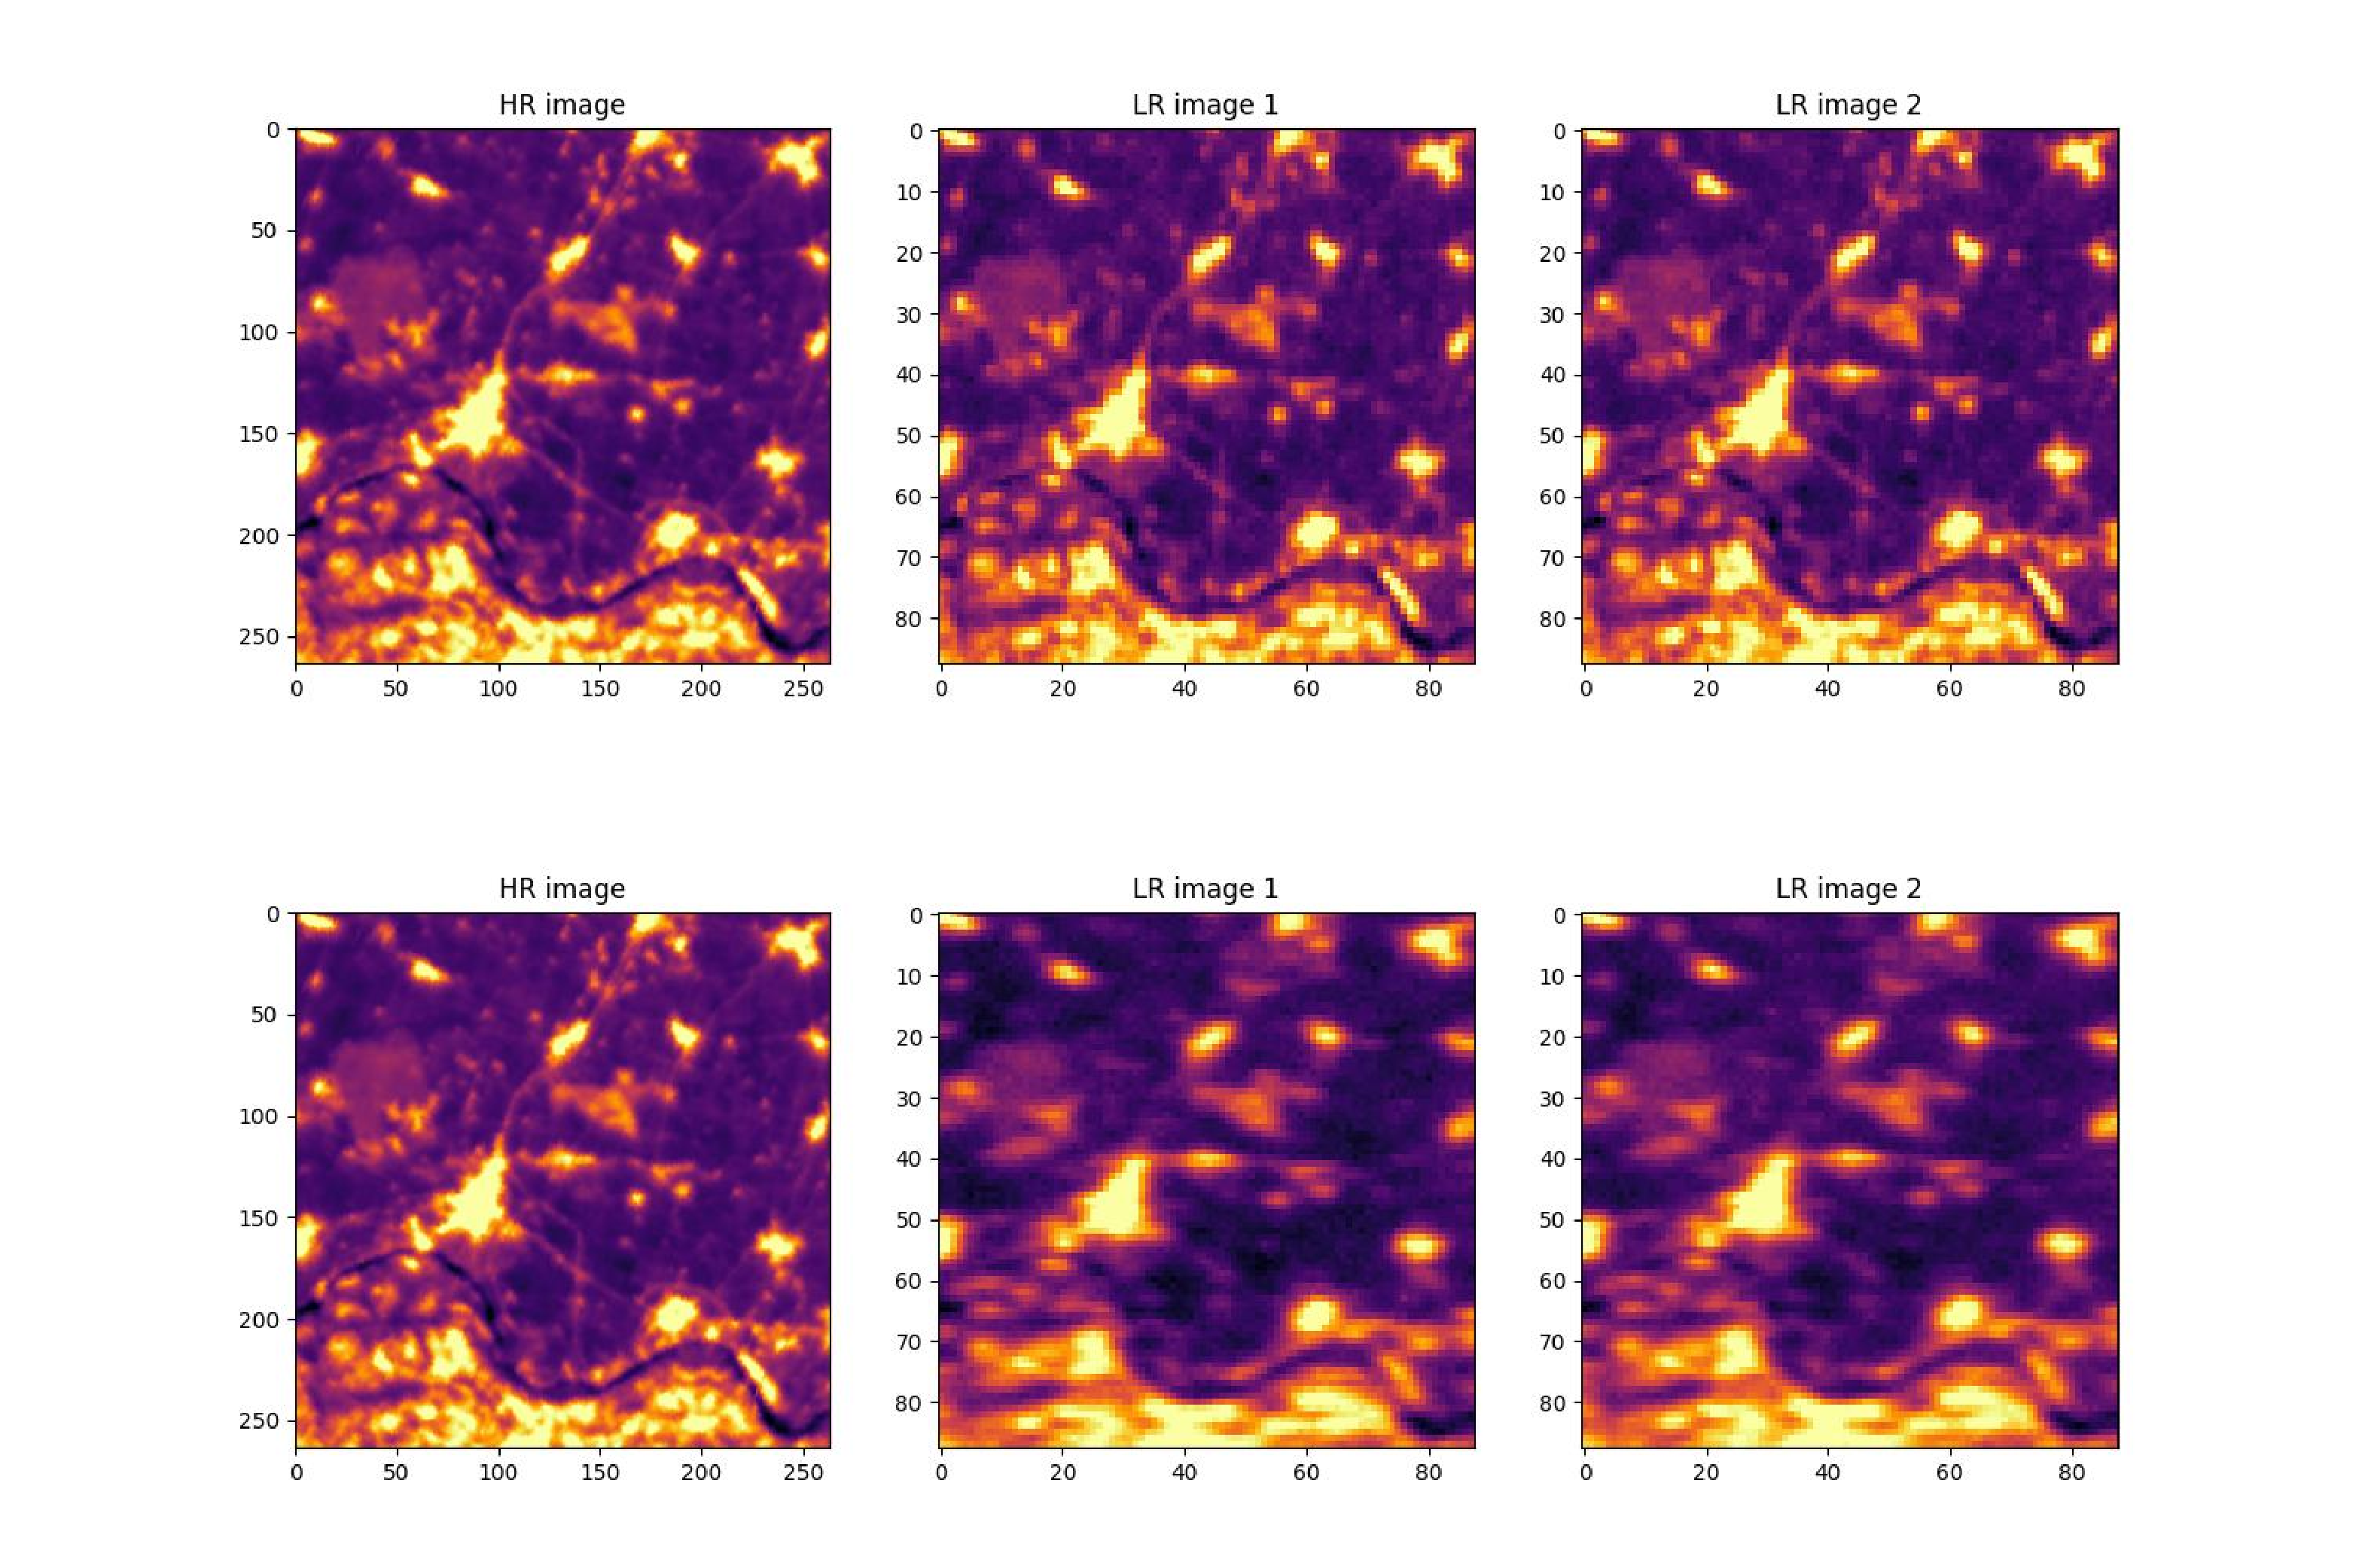
\includegraphics[width=\linewidth]{Includes/4-degradation-kernel-examples.pdf}
                \caption{Effects of different blurring kernels on the HR-LR generation. The upper row contains images generated using blurring kernels with symmetric distributions. The lower rows contain images generated using asymmetric distributions, resulting in highly anisotropic kernels.}
                \label{fig:4-degradation-kernel-examples}
            \end{figure}
            
        \subsubsection{Radiometric error correction}

        FOREST-2 radiometric accuracy is 1K at 300K.
        Other missions report higher nominal radiometric accuracy, such as the case of the ECOSTRESS instrument sheet \cite{ECOSTRESS2023INSTRUMENT}, which is 0.5K at 300K.
        This difference in accuracy should be taken into account. For this, the additional error required is calculated using the following equation:

        \begin{equation}
            e_{\text{forest}} = \sqrt{e_{\text{eco}}^2 + e_{\text{extra}}^2} 
            \label{eq:4-radiometric-error-correction}
        \end{equation}
        
        Where $e_{\text{eco}}$ is the ECOSTRESS error, and $ e_{\text{extra}}$ is the additional error required for FOREST-2.
        
        Using the above equation, an additional radiometric error of approximately 0.8660K is needed. The next step involves converting the extra error into a radiance value, by calculating the derivative of the Planck equation at 300K, which is done numerically as follows:
        
        \begin{equation}
            \frac{\partial B}{\partial T} = \frac{B(\lambda, T + \delta T) - B(\lambda, T)}{\delta T}
            \label{eq:4-planck-derivative}
        \end{equation}  
        
        Multiplying the results of equations \ref{eq:4-radiometric-error-correction} and \ref{eq:4-planck-derivative}, the radiance error for both FOREST LWIR bands is obtained. The additional radiance errors for LWIR1 and LWIR2 bands are found to be \(1.5472 \times 10^{-1}\) W/sr/m\(^2\)/\(\mu m\) and \(1.1444 \times 10^{-1}\) W/sr/m\(^2\)/\(\mu m\), respectively.

        The difference in radiance will be split into two components. On one side, the cold bias represents a systematic error in the measurement; this error acknowledges discrepancies that can be attributed to sensor calibration and atmospheric conditions. On the other side, the random noise accounts for unpredictable fluctuations in the measurement process. This could be due to a variety of sources like electronic noise in the sensor, random atmospheric disturbances, or other stochastic factors. As the extent of each component is not known and to give more variability to this basic degradation model, a random factor $\phi \in [0,1] $ is introduced:

        \begin{equation}
        \begin{aligned}
            \varepsilon_{\text{final}} &= (1 - \phi) \times \varepsilon_{\text{radiance}} + \phi \times \eta \times \varepsilon_{\text{radiance}} \\
            \eta & \sim \mathcal{N} (0,1)
        \end{aligned}
        \end{equation}    

        The effects of the error correction are shown in Fig. \ref{fig:4-radiometric_noise_example}. As the target radiometric error increases, the loss of information is more noticeable.


        \begin{figure}[h!]
            \centering
            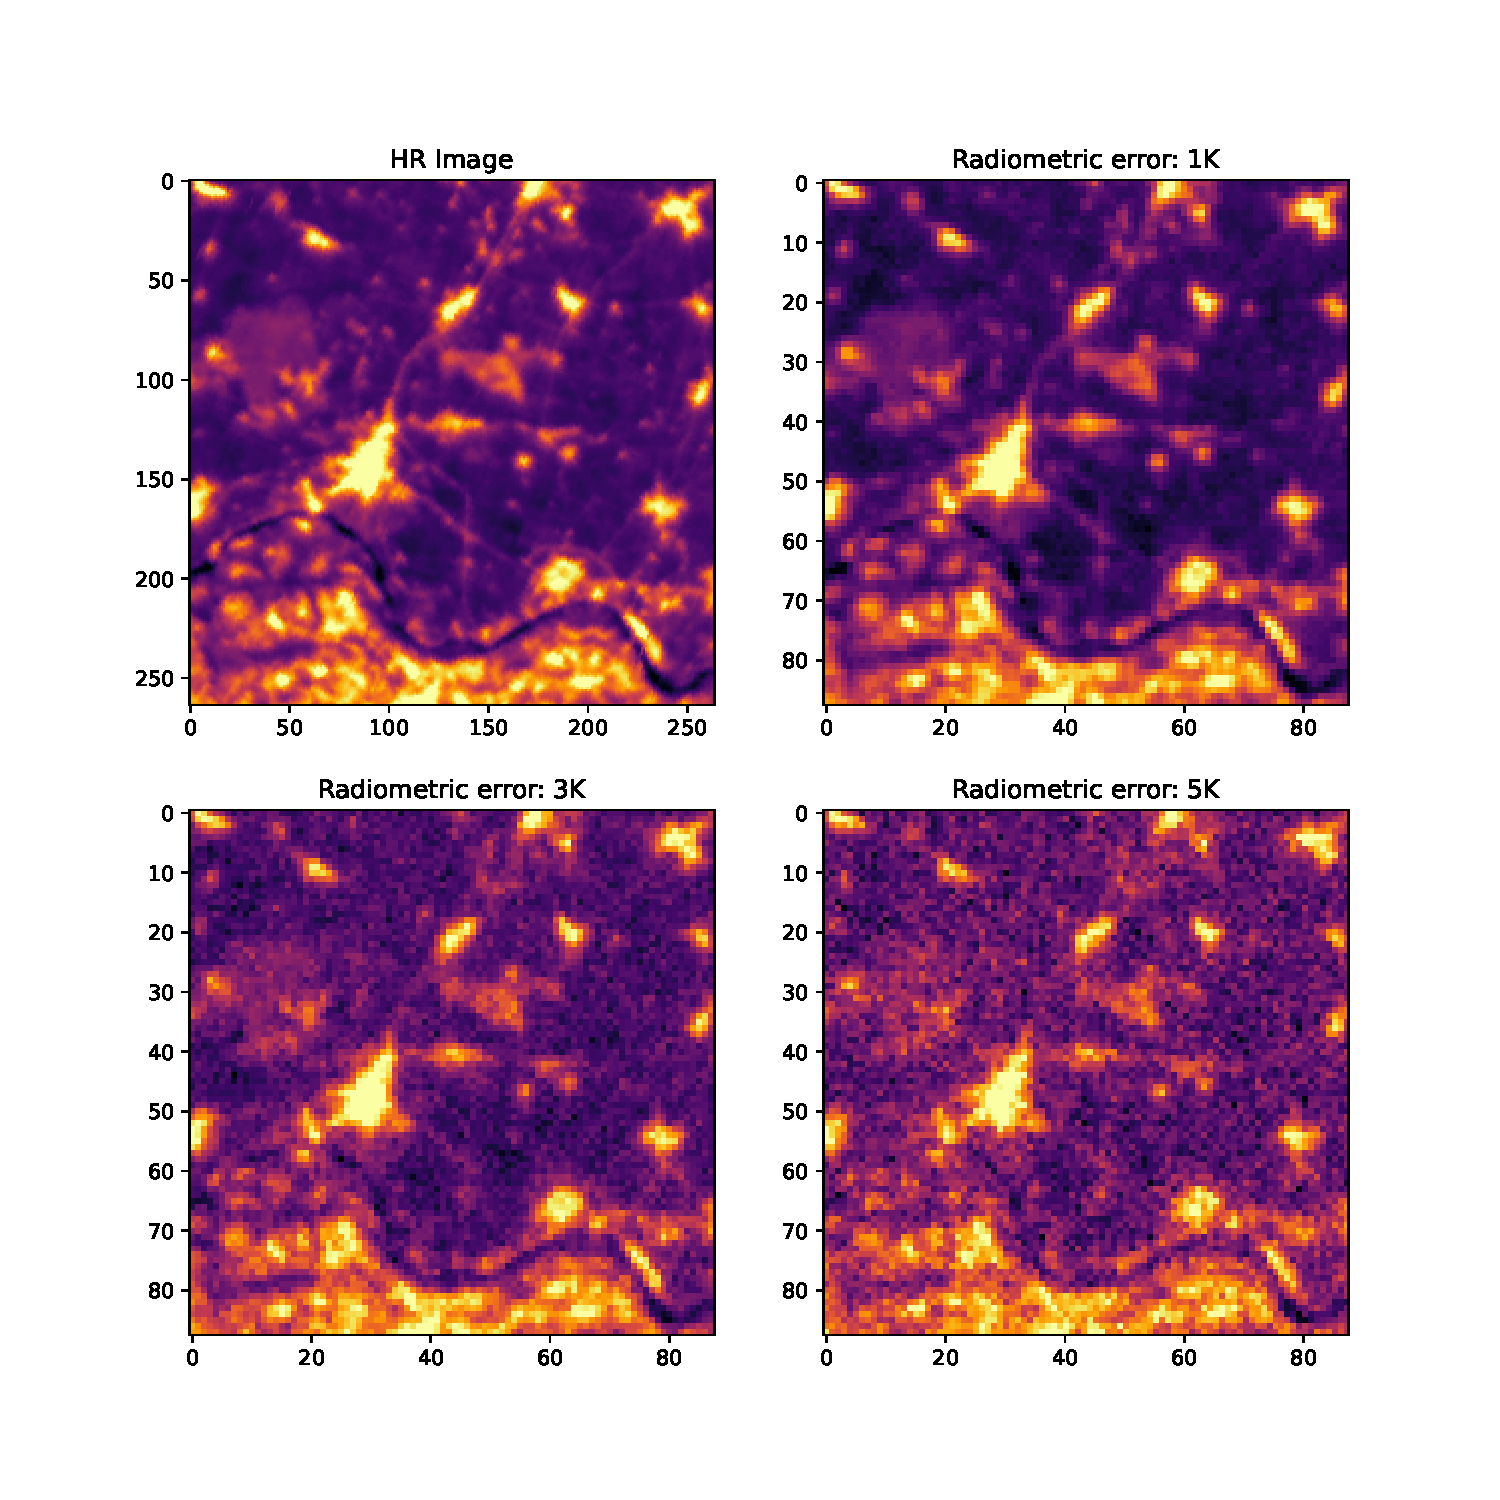
\includegraphics[width=\textwidth]{Includes/4-radiometric_noise_example.pdf}
            \caption{Effects of increasing radiometric error on the HR-LR generation.}
            \label{fig:4-radiometric_noise_example}
        \end{figure}
        
    

    \subsection{Signal-to-noise ratio }

        The Signal-to-Noise Ratio (SNR) is commonly used to quantify how much a signal is corrupted by noise. It is defined as the ratio of signal power to noise power and is usually expressed in decibels (dB). Mathematically, the SNR is often defined as:

        \[ \text{SNR} = 10 \log_{10} \left( \frac{P_{signal}}{P_{noise}} \right) \]

        Where $P_{signal}$ and $P_{noise}$ represent the power of the signal and the noise tensors, calculated as the sum of their squared elements.
        A higher SNR indicates a more distinguishable signal in comparison to the noise. In the context of this work, it will be used to assess the power of the noise introduced by the probabilistic degradation model compared to the clean image.

    \subsection{Referenced image quality metrics}

        When the HR image is available, the performance of a super-resolution algorithm can be evaluated using a variety of metrics. 
        These metrics can be divided into two categories: pixel-based and perceptual-based.
        Pixel-based metrics are based on the pixel-wise comparison between the generated image and the ground truth. 
        Perceptual-based metrics, on the other hand, are based on the perceptual similarity between the generated image and the ground truth. 
        These metrics are built using a pre-trained deep neural network, which is usually trained on a large dataset of images.
        The following sections will describe the most commonly used metrics in the literature.

        \subsubsection{Pixel-wise losses}

            The $L_1$ and $L_2$ losses are the most commonly used pixel-based metrics in the literature. 
            Additionally, they are the most common loss function that drives the super resolution network gradients during training. 
            In a general form, the $L_1$ and $L_2$ losses are defined as follows:

            \begin{equation}
                \mathcal{L}_{L_p} = \frac{1}{H \cdot W} \sum_{i=1}^{H} \sum_{k=1}^{W} |I^{\text{HR}}_{i,k} - I^{SR}_{i,k}|^p
            \end{equation}

            Where $I^{\text{HR}}_{i,k}$ and $I^{SR}_{i,k}$ are the ground truth and the super-resolved image at the pixel position [i,k], and $p$ is the exponent of the loss function. 
            The $L_2$ loss weights high-value differences higher than low-value differences due to the exponent of two, resulting in an excessively smooth loss for low values and considerable variability for high values.
            For that reason, it is more common to see the $L_1$ loss being used in the SR literature and is the one employed in the experiment.

        \subsubsection{Adversarial loss}

        In order to train the probabilistic degradation model GAN, an adversarial loss must be used. 
        Viewing the discriminator as a classifier, the original GAN implementation uses the cross-entropy loss. This will cause the problem of vanishing gradients in the generator when the samples are on the correct side of the decision boundary but are still far from the real data. For that reason, the LSGAN is proposed in \cite{mao2017squares}. 
        
        Benefits of LSGANs include the penalization of samples that are on the correct side of the decision boundary but far from it. This will generate more considerable gradients in the generator update, relieving the vanishing gradients problem. As a result, the learning process is more stable and will create higher quality images from the generator.

        

        \subsubsection{Peak signal-to-noise ratio}

         
            Peak Signal-to-Noise Ratio (PSNR) measures the magnitude of the error compared with the reference image. It is usually used to quantify the amount of error or noise introduced during the image reconstruction process.
            
            PSNR is calculated by first computing the Mean Squared Error (MSE) or $\mathcal{L}_2$ loss between an image and the reference and then taking the logarithmic ratio of the maximum possible pixel value squared. The PSNR value is usually expressed in decibels (dB). The formula for PSNR is:
            
            \begin{equation}
            PSNR = 10 \cdot \log_{10} \left( \frac{I_{MAX}^{2}}{\mathcal{L}_2} \right)
            \end{equation}
            
            Where $I_{MAX}$ is the maximum possible pixel value of the reference image, and $\mathcal{L}_2$ is the mean squared error between the image and the reference. A higher PSNR value indicates a better quality of the super-resolved image, as it signifies a lower level of noise or error. However, it's worth noting that it may not always align with human perceptual evaluations of image quality, as it focuses on physical consistency.

        \subsubsection{Structural similarity index}

            
        Structural Similarity Index Measure (SSIM) takes into consideration changes in structural information, luminance, and contrast. By doing this, it manages to reflect the perceived changes in noise level and contrast better.
        The SSIM index is calculated by dividing the image into windows of a certain size and then comparing corresponding windows in the reference and target images. The SSIM index for a pair of windows, say $x$ and $y$, is given by:
        
        \begin{equation}
            SSIM(x, y) = \frac{(2\mu_x\mu_y + c_1)(2\sigma_{xy} + c_2)}{(\mu_x^2 + \mu_y^2 + c_1)(\sigma_x^2 + \sigma_y^2 + c_2)}
        \end{equation}
        
        Where $\mu_x$ and $\mu_y$ are the average pixel values, $\sigma_x^2$ and $\sigma_y^2$ are the variances, $\sigma_{xy}$ is the covariance of $x$ and $y$, and $c_1, c_2$ are small constants to avoid division by zero.
        The final SSIM score for the images is calculated by averaging the SSIM indices of all windows. An SSIM score of 1 indicates a perfect structural match between the two images, whereas a score of 0 indicates no structural similarities.

        \subsubsection{Learned perceptual image patch similarity}

        LPIPS is a perceptual metric that leverages deep learning to compute perceptual differences between images. Specifically, it uses the activations of a pre-trained convolutional neural network (in this case, VGG \cite{VGGnet} ) to extract perceptual features from the images afterwards. 
        Then, it calculates the Euclidean distance between these feature vectors to measure the perceptual difference.
        This measure has gained popularity in SR tasks due to its high correlation with human judgments of visual similarity \cite{zhang2018unreasonable}.
        
        The LPIPS score is given by:
        
        \begin{equation}
        LPIPS(I^{HR}, I^{SR}) = \sqrt{\sum_{i=1}^{N} w_i\|f_i(I^{HR})-f_i(I^{SR})\|^2}
        \end{equation}
        
        where $I^{HR}$ and $I^{SR}$ are the images being compared, $f_i(I)$ denotes the $i$-th layer activation when image $I$ is the input to the pre-trained network, $N$ is the number of layers considered, and $w_i$ is the learned weight for the $i$-th layer.
        
        A lower LPIPS score indicates a lower distance between the feature vectors and, thus, a greater perceptual similarity between the two images. 
        Due to the fact that in this work, we are interested in the physical consistency of the super-resolved images, 
        this metric will be shown but will not drive any decision during the training process.
        

        \subsubsection{Translation and bias adjustment}\label{subsec:adjustedmetrics}
    
            In order to calculate the losses and performance metrics, the generated test images are compared against the HR images.
            Additional changes should be considered, particularly in a MISR environment \cite{martens2019superresolution}.
            Minor shifts in the contents of the pixels are expected, and  SR methods may have undesired effects on the border pixels. Therefore, metrics should have some tolerance to small pixel translations in the high-resolution space by evaluating a sliding cropped image. 
            This implies looking for a displacement of SR by at most $d$ pixels in each direction and picking the one that minimizes the error. 
            An example of how this is applied in a loss that needs to be minimized can be found in Eq. \ref{eq:4_adjusted_metrics}
    
            \begin{equation}
               \mathcal{L}^* ( I^{HR}, I^{LR}, d) = \min_{u,v \in [0,2d]} \mathcal{L} ( I^{HR}_{u,v}, I^{SR}_{u,v})
            \label{eq:4_adjusted_metrics}
            \end{equation}
    
            Additionally, commonly used metrics punish biases as much as noise in the reconstruction.
            For example, if $I^{SR} = I^{HR} + \epsilon$, where $\epsilon$ is a constant bias, a perfect reconstruction of $I^{SR}$ is possible if $\epsilon$ is known. 
            A quality metric should award a high score to super-resolved outputs with these characteristics in comparison to the introduction of noise and information loss. Metrics like L2/L1 losses and PSNR do the exact opposite and thus should incorporate a bias compensation like the following: 
    
            \begin{equation}
                \begin{aligned}
                    \mathcal{L}^* ( I^{HR}, I^{LR}, d) = \min_{u,v \in [0,2d]} \mathcal{L} ( I^{HR}_{u,v}, (I^{SR}_{u,v}+b)) \\
                    b = \frac{1}{(W - d)(H - d)} \sum_{x,y} \left( I^{HR}_{u,v} - I^{SR}_{u,v} \right)
               \end{aligned}
            \end{equation}
    
            \noindent Where $W$ and $H$ represent the width and height of the image, respectively.
    

    \subsection{Non-referenced image quality metrics}

    Non-Referenced Image Quality Assessment (NRIQA) aims to develop methods to measure image quality in alignment with human perception without the need for an HR reference. 
    Most of them are based on two steps: feature extraction and quality prediction using a regression module. 
    They rely on the assumption that natural images share certain statistical information and that any distortion may alter these statistics \cite{niqe}.
    The results from an arbitrary image are compared to a default model trained on a large dataset of natural scenes, and the difference between them is used to predict the quality of the image.
    % In recent years, researchers have relied on deep learning to perform the two steps in a single model. 
    % The workflow of these models is shown in Fig. \ref{fig:4-nr-iqa-workflow}.

    % \begin{figure}[h!]
    %     \centering
    %     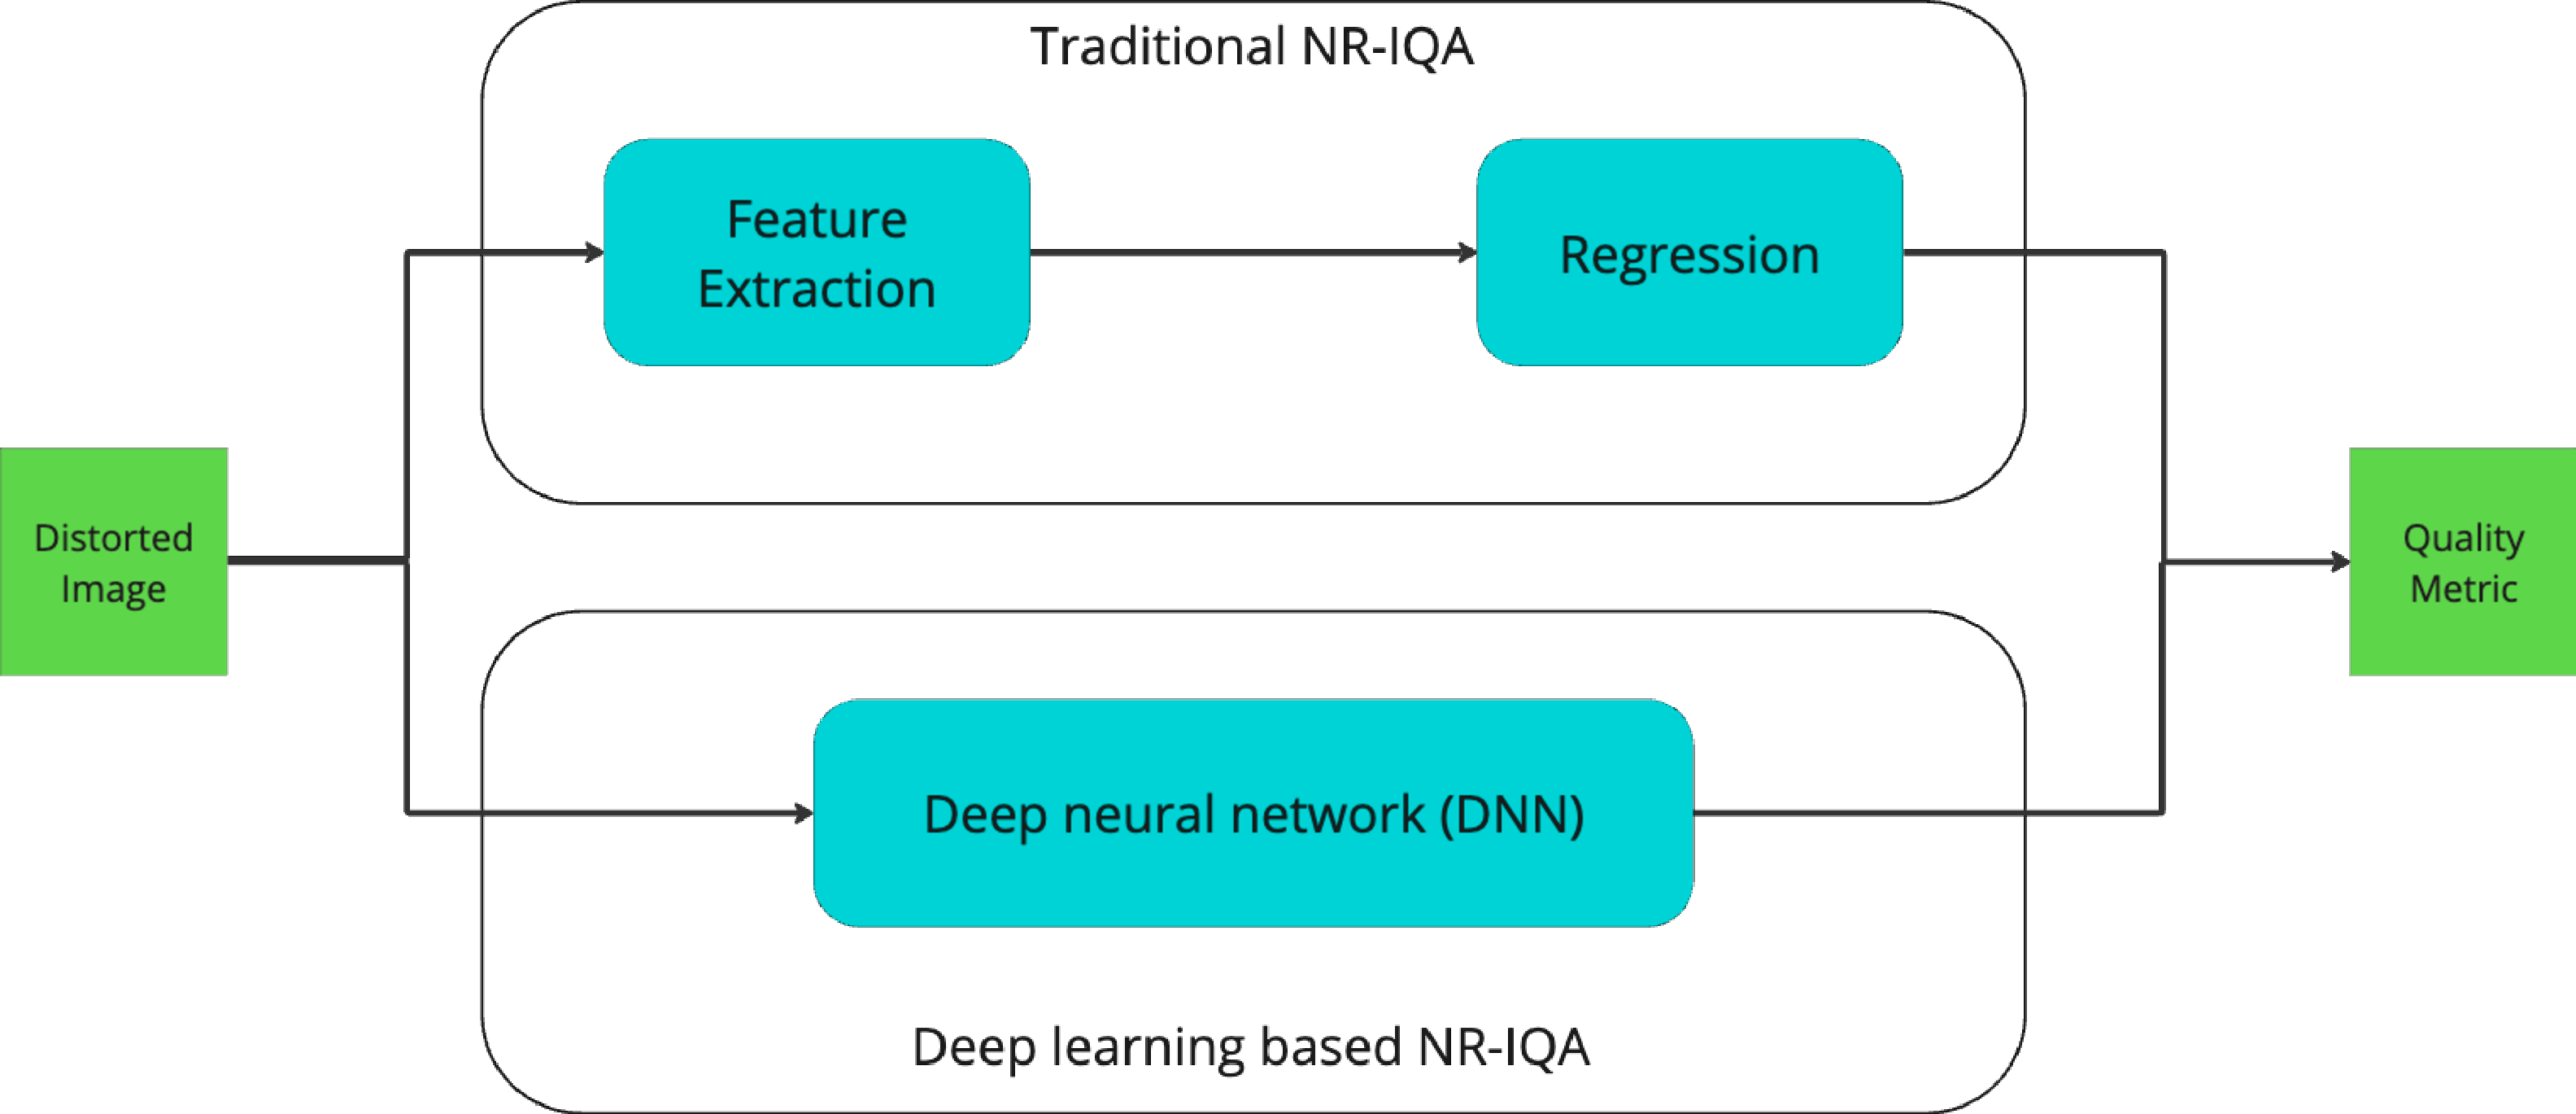
\includegraphics[scale=0.25]{Includes/3-NR-IQA.pdf}
    %     \caption{Workflow of an NR-IQA model.}
    %     \label{fig:4-nr-iqa-workflow}
    % \end{figure}


        

        \subsubsection{Naturalness image quality evaluator}

        
            The Naturalness Image Quality Evaluator (NIQE) \cite{niqe} operates on the principle that pristine natural images exhibit specific statistical properties that can be quantified to establish a benchmark for quality assessment. 
            NIQE employs a model based on a multivariate Gaussian distribution characterized by a mean vector and covariance matrix to represent the statistical attributes of a natural image's visual patterns.
            To assess its quality, NIQE extracts a corresponding set of features and evaluates their deviation from this statistical model using the Mahalanobis distance.
            This distance measures the divergence of the image's features from those typical of high-quality natural images.
            A lower value suggests that the image closely resembles the statistical properties of natural images, indicating higher perceived quality. This provides a measure of image quality that aligns with the naturalness of human visual perception. 

        \subsubsection{Blind/referenceless image spatial quality evaluator}

            Similar to NIQE, the Blind/Referenceless Image Spatial Quality Evaluator (BRISQUE) \cite{mittal2012} operates on the premise that natural images possess specific statistical properties that are altered in the presence of distortions. It operates by quantifying deviations from the statistical regularities observed in natural images, primarily using locally normalized luminance coefficients. 
            Following this, a spatial domain model is utilized to calculate a set of features that are designed to capture the loss of naturalness due to the presence of distortions.
            These extracted features are fed into a Support Vector Regression (SVR) that was trained with a set of images with known quality ratings to predict the quality score of the image.
            
            A lower BRISQUE score is indicative of better quality, implying that the image has a better quality score in the pre-trained model. The main difference between BRISQUE and NIQE is that BRISQUE uses the SVR model and directly predicts the quality score, while NIQE calculates the distance between the multivariate Gaussian distribution model of the image and the one from the specific dataset where the evaluator was pre-trained.




        \subsection{Frequency domain analysis} \label{subsubsec:frequency_domain_analysis}
        
        The Fourier transform is widely used to analyze the frequency content of signals.
        It can also be applied to multidimensional signals such as images, where the spatial variations of pixel intensities have a unique representation in the frequency domain. 
        The objective of the super resolution is to reconstruct missing high-frequency components from an LR image.
        A good SR algorithm seeks to amplify the high-frequency components compared to a baseline such as bicubic interpolation while keeping noise at bay.
        The Fourier components provide global information about the image, as opposed to local information represented by pixel values in the spatial domain \cite{fuoli2021fourier}. 
        
        Using the Fast Fourier Transform (FFT), the pixel intensity values of super-resolved images are converted into a spectrum where each point represents a specific frequency contained in the spatial domain.
        The FFT is then shifted so that the zero-frequency component is at the center of the spectrum. 
        The resulting magnitude reveals the energy distribution across various frequencies and is usually visualized in grayscale, where the intensity corresponds to the amplitude of the frequency components.
        
        A radial profile of the FFT magnitude provides insights into how different spatial frequencies contribute to the image content.
        The radial profile calculates the average intensity of frequencies at a given radius from the center of the Fourier transform and depicts the average magnitude of a given frequency in all possible directions. This metric serves as a benchmark for evaluating the performance of SR techniques against traditional interpolation methods such as bicubic interpolation.
        
        Spatial frequency within an image context refers to the periodicity of the intensity variation over spatial dimensions, typically quantified in cycles per pixel. The central region of the frequency domain, after the shift operation, denotes the zero frequency. In contrast, the edges of the FFT image represent the highest frequencies, constrained by the image's discrete sampling rate.
        To quantitatively interpret these spatial frequencies, a radial-to-frequency mapping is necessary. This mapping accounts for the Nyquist frequency, which is delineated as half the sampling rate of the discrete imaging grid composed of squared pixels.

        It is important to note that given the 2D nature of an image, the Nyquist limit is not the same in all directions. 
        Along each axis, the Nyquist limit is 0.5 cycles per pixel. Still, in a diagonal direction, the limit is reached by combining the spatial frequency of the $x$ and $y$ axis, which is at $\frac{\sqrt{2}}{2} \approx 0.707$ cycles per pixel. 
        This means that frequencies above 0.5 cycles per pixel can be detected only if their direction is not along any of the axes.
        The effect of the Nyquist limit can be seen in Fig. \ref{fig:5-square_vs_radial}. The maximum possible frequency in an FFT plot of a squared image is in the corners. However, when normalized by the direction-dependent Nyquist limit, the maximum is reached in the borders of the FFT.

        \begin{figure}[H]
            \centering
            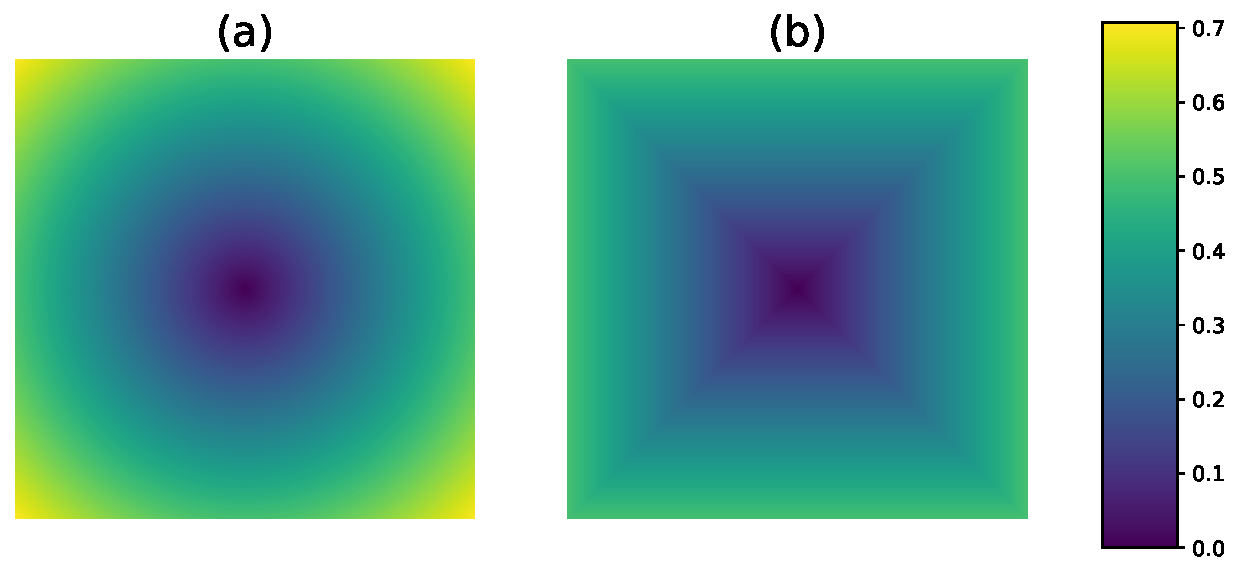
\includegraphics[width=\linewidth]{Includes/5-square_vs_radial.pdf}
            \caption{Comparison between (a) the radial representation of frequencies in cycles per pixel and (b) the frequency normalized by the direction-dependent Nyquist limit. The frequency limit is always on the borders of the FFT plot, but they represent different frequency values depending on the direction.
            }
            \label{fig:5-square_vs_radial}
        \end{figure}
        
        
        The conversion of a given radius in the FFT output to the corresponding spatial frequency is formalized as:

        \begin{equation}
            f(r) = \frac{r}{\frac{N}{2}} \cdot f_{\text{Nyquist}},
        \end{equation}

        Where \( f(r) \) signifies the spatial frequency associated with radius \( r \), \( N \) represents the FFT image dimension, assuming a square configuration, and \( f_{\text{Nyquist}} \) the Nyquist frequency, which is 0.5 cycles per pixel along the $x$ and $y$. An example of the procedure is shown in \ref{fig:4-frequency-analysis}. Usually, frequencies higher than 0.5 cycles per pixel have a low log magnitude and can be disregarded in the analysis.

        \begin{figure}[H]
            \centering
            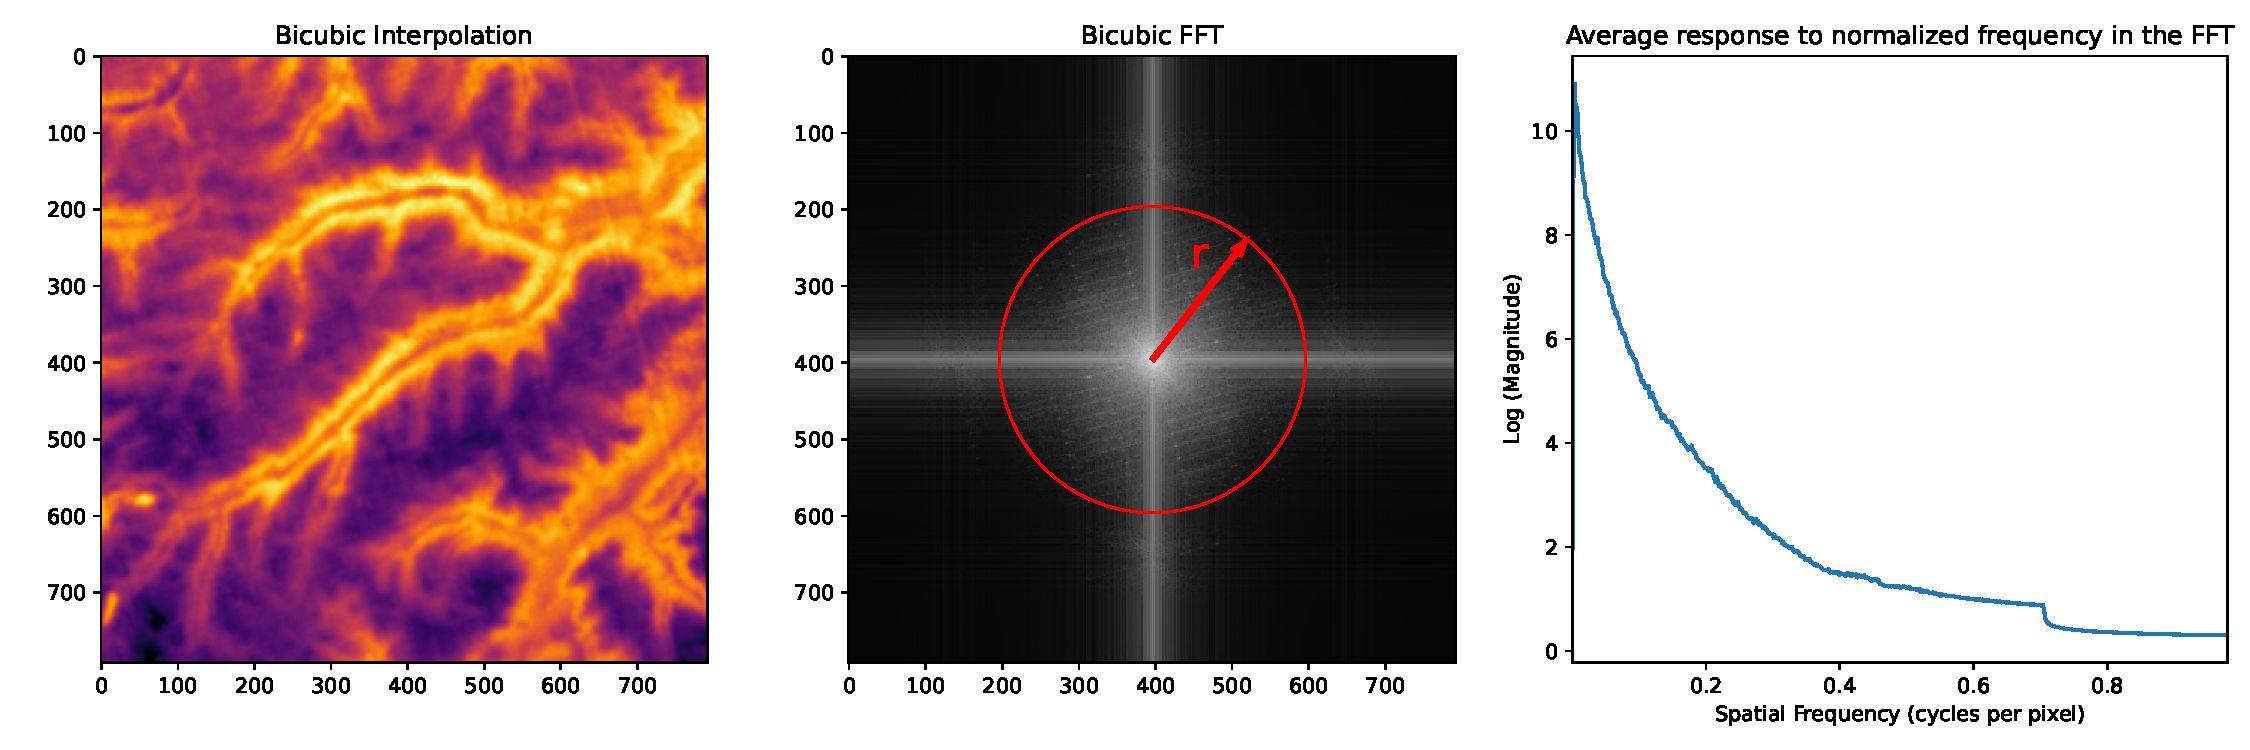
\includegraphics[width=\linewidth]{Includes/4-frequency-analysis.pdf}
            \caption{Steps of the frequency domain analysis. (b) shows the log magnitude of the shifted FFT of the scene depicted in (a). The radial profile is calculated by averaging all the points that have the same $r$. In (c), the log magnitude obtained for every radial profile is plotted, translating the axis from radius into spatial frequency.}
            \label{fig:4-frequency-analysis}
        \end{figure}
        

        Through FFT, a depiction of the amplification or attenuation of frequencies attributable to the SR techniques can be calculated. 
        Analyzing these profiles displays the ability of SR models to enhance details. 
        However, it is essential to note that this method does not account for artifacts generated by the super resolution process and should be used in combination with other metrics.

        \subsection{Gradient distribution analysis}


        An alternative way of analyzing super resolution results is by looking at the gradients of the images. 
        HR images are sharper, and thus, each pixel on average, has higher gradient magnitudes in both directions compared to their LR counterparts.
        A super-resolution algorithm should increase the sharpness of the edges, resulting in a gradient distribution that aligns more closely with that of the genuine HR image.
        
        An approximation of the gradients can be estimated by doing 2D convolutions between an image and Sobel kernels, as displayed in Eq. \ref{eq:4-sobel-operators} \cite{Sobel1990AnI3}.
        These kernels are designed to respond maximally to edges running vertically and horizontally relative to the pixel grid.
        
        \begin{equation}
            \begin{array}{ccc}
            \hat{G}_x = \begin{bmatrix}
            -1 & 0 & +1 \\
            -2 & 0 & +2 \\
            -1 & 0 & +1
            \end{bmatrix}
            &
            \quad
            &
            \hat{G}_y = \begin{bmatrix}
            +1 & +2 & +1 \\
             0 &  0 &  0 \\
            -1 & -2 & -1
            \end{bmatrix}
            \end{array}
            \label{eq:4-sobel-operators}
        \end{equation}
    
         The kernels can be applied separately to the input image to produce the component of the gradient in each orientation $G_x$ and $G_y$. The magnitude of the gradient  is given by: 
         \begin{equation}
             |G| = \sqrt{G_x^2 + G_y^2}
             \label{eq:4-gradient_magnitude}
         \end{equation}

         The gradient magnitude histograms of the results of different super resolution algorithms will be assessed, thereby quantifying the enhancement in edge sharpness.
         This histogram provides insights into the frequency and intensity of the edges within an image.
         A better SR model should demonstrate a histogram with larger gradient magnitudes, indicating sharper edges.
         However, it is important to note that this analysis is unsupervised and disregards the effect of noise and artifacts introduced during the super-resolution process. Thus, it should be considered in combination with other metrics.

         \begin{figure}[H]
             \centering
             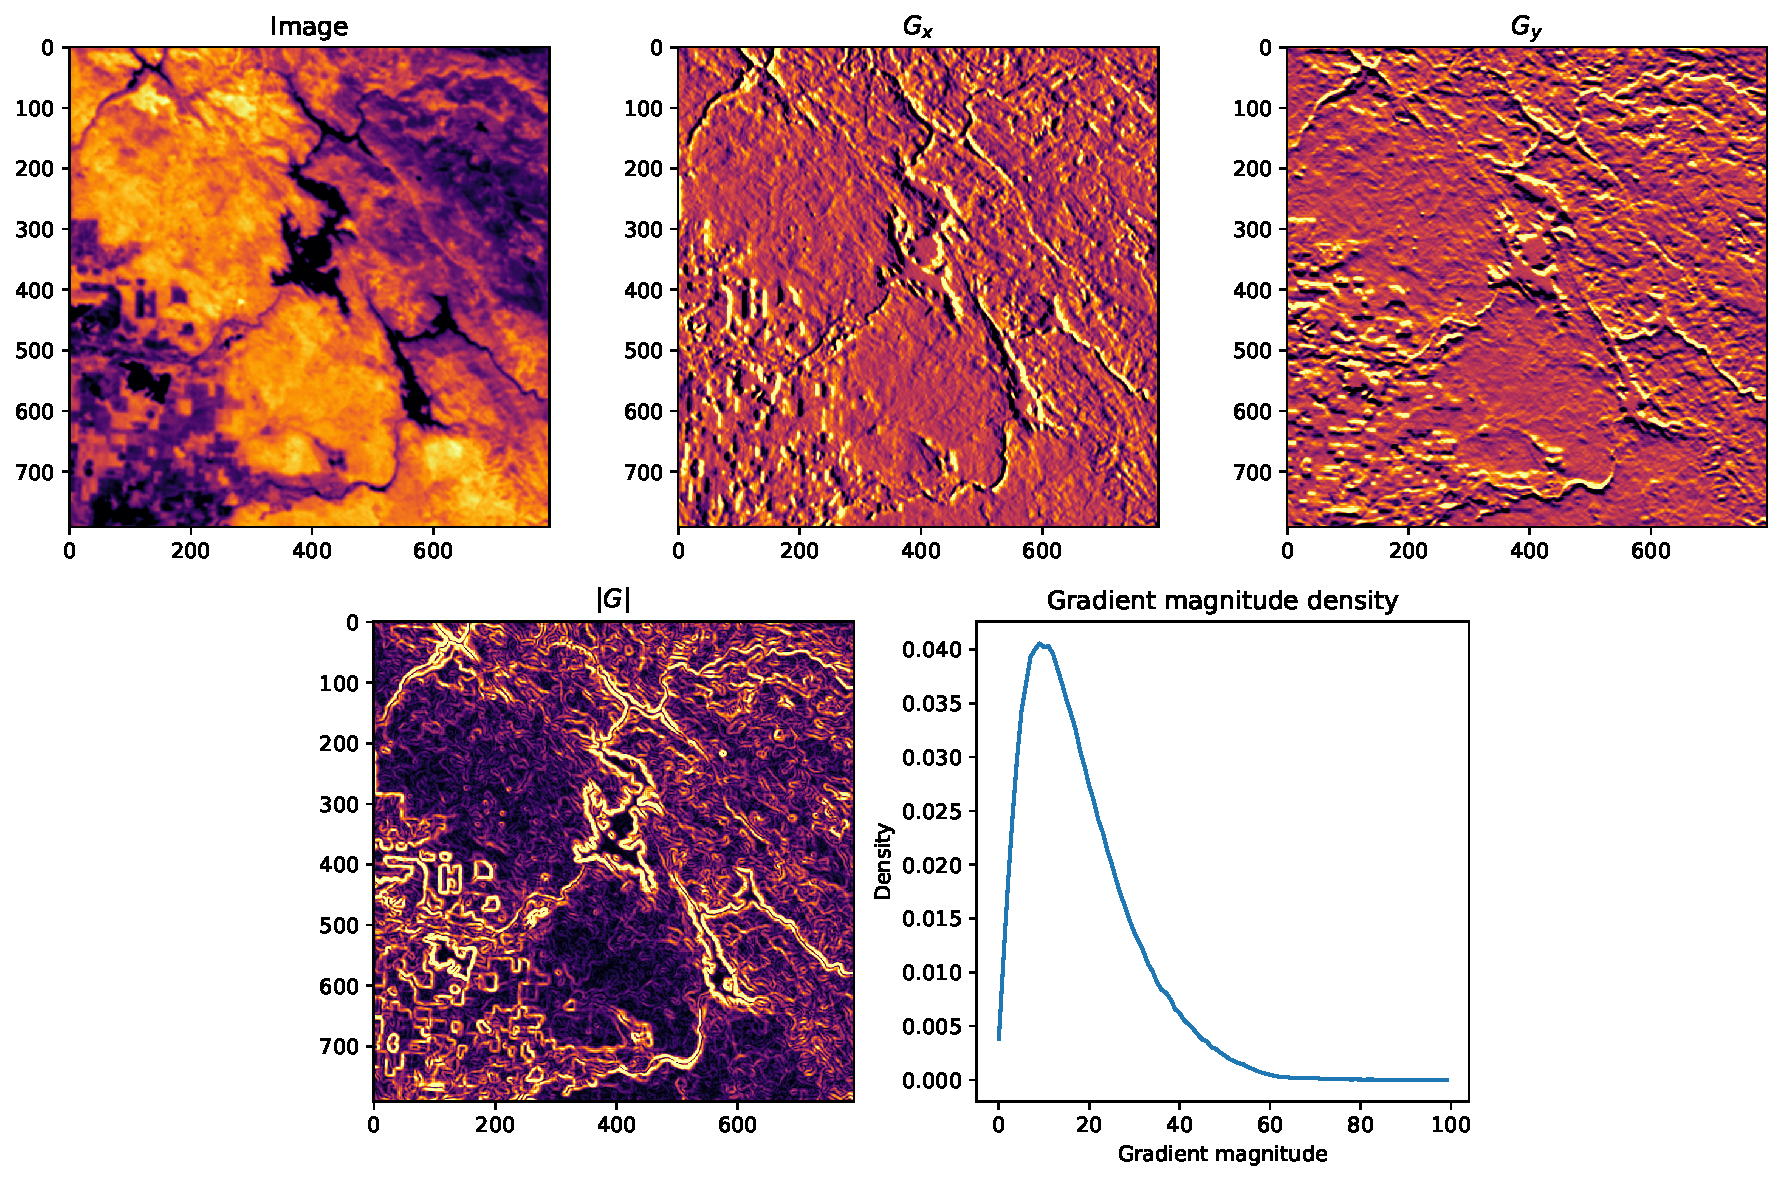
\includegraphics[width=\textwidth]{Includes/4-gradient-analysis.pdf}
             \caption{Steps to obtain a gradient magnitude density. Using the Sobel operators, $G_x$ and $G_y$ are obtained from an image. The magnitude $|G|$ of each pixel is calculated using Eq. \ref{eq:4-gradient_magnitude}. The density can be estimated afterward, using 100 bins in this case.}
             \label{fig:4-gradient-analysis}
         \end{figure}


      \subsection{Correlation between pixel and neighbors }


        In a similar fashion to the gradient analysis, kernels can be used to estimate the correlation between the pixels of an image and their neighbors. The Pearson correlation coefficient between the results of the convolutions of the image and the following kernels will be calculated.
        
        \begin{equation}
            \begin{array}{ccc}
            \hat{G}_{center} = \begin{bmatrix}
            0 & 0 & 0 \\
            0 & 1 & 0 \\
            0 & 0 & 0
            \end{bmatrix}
            &
            \quad
            &
            \hat{G}_{neighbors} = \begin{bmatrix}
             1/8 &  1/8 & 1/8 \\
             1/8 &  0 & 1/8 \\
            1/8 & 1/8 & 1/8
            \end{bmatrix}
            \end{array}
            \label{eq:4-correlation-operators}
        \end{equation}
    
         In an image, a high correlation coefficient is expected, as the content of a pixel is highly dependent on its neighbors. However, images with higher definition have sharper edges, and thus, their correlation coefficient should be lower in comparison. It is important to note that this analysis does not take into account the noise present in the image, as it will reduce the correlation coefficient without improving the image quality. In an extreme case, an image composed only of white noise would have a correlation coefficient between each pixel and its neighbors of 0. Despite this, it is helpful to understand the super resolution process.
         

\clearpage

        

        
        

\section{Datasets}

\subsection{Obtaining a high-resolution dataset}
    
    
Super resolution is inherently a supervised learning task that needs the availability of high-resolution (HR) data. In scenarios where HR data from sources like FOREST-2 is unavailable, an alternative is to generate synthetic images from external missions with characteristics similar to the FOREST-2 mission but with a superior spatial resolution.

\subsubsection{The ECOSTRESS mission}

NASA's ECOsystem Spaceborne Thermal Radiometer Experiment on Space Station (ECOSTRESS) mission is designed to provide new insights into the effects of the Earth's climate dynamics \cite{ECOSTRESS2023}, with a focus on the following scientific objectives:

\begin{enumerate}
    \item Identify the critical thresholds of water use and water stress in key climate-sensitive biomes, typically by observing the transition zones between biomes.
    \item Identify when plants stop taking up water over the course of a day.
    \item Improve the accuracy of drought estimates based on agricultural water use in the continental United States. 
\end{enumerate}

ECOSTRESS employs thermal infra-red radiometers, specifically Prototype HyspIRI Thermal infra-red Radiometer \cite{PhyTIR2023} to measure the radiation emitted from the Earth's surface. It provides a spatial resolution of 69 meters with a temperature sensitivity of a few tenths of a degree \cite{ECOSTRESS2023}. The swath size is 400x400 km. The detector separates the energy from five different wavelengths using filters attached to the detector, producing five separate image layers for each scene. The pixels represent the intensity of thermal infra-red radiation emitted by the Earth's surface at each wavelength. The mission has a 4-day diurnal repeat cycle.

In the spatial domain, ECOSTRESS constitutes an excellent candidate for generating synthetic HR images, as its resolution constitutes approximately a threefold increase compared to FOREST-2. 

In the spectral domain, it is crucial to confirm the overlap between the mission bands. Given the narrower ECOSTRESS bands, the strategy will be averaging the radiances to align the spectral properties.
Fig. \ref{fig:5-wavelength-comparison} shows this spectral band comparison.
In the case of the LWIR1 FOREST band, the overlap is significant with the first three ECOSTRESS bands.
Although the overlap is less pronounced in the LWIR2 band, the radiation spectrum of black bodies at prevalent surface temperatures suggests the feasibility of constructing a synthetic LWIR2 from the last two ECOSTRESS bands.

While FOREST's temporal resolution exceeds that of ECOSTRESS, allowing for the monitoring of new processes, this aspect is not the primary focus of the current study and will not be taken into account.



\begin{figure}[H]
    \centering
    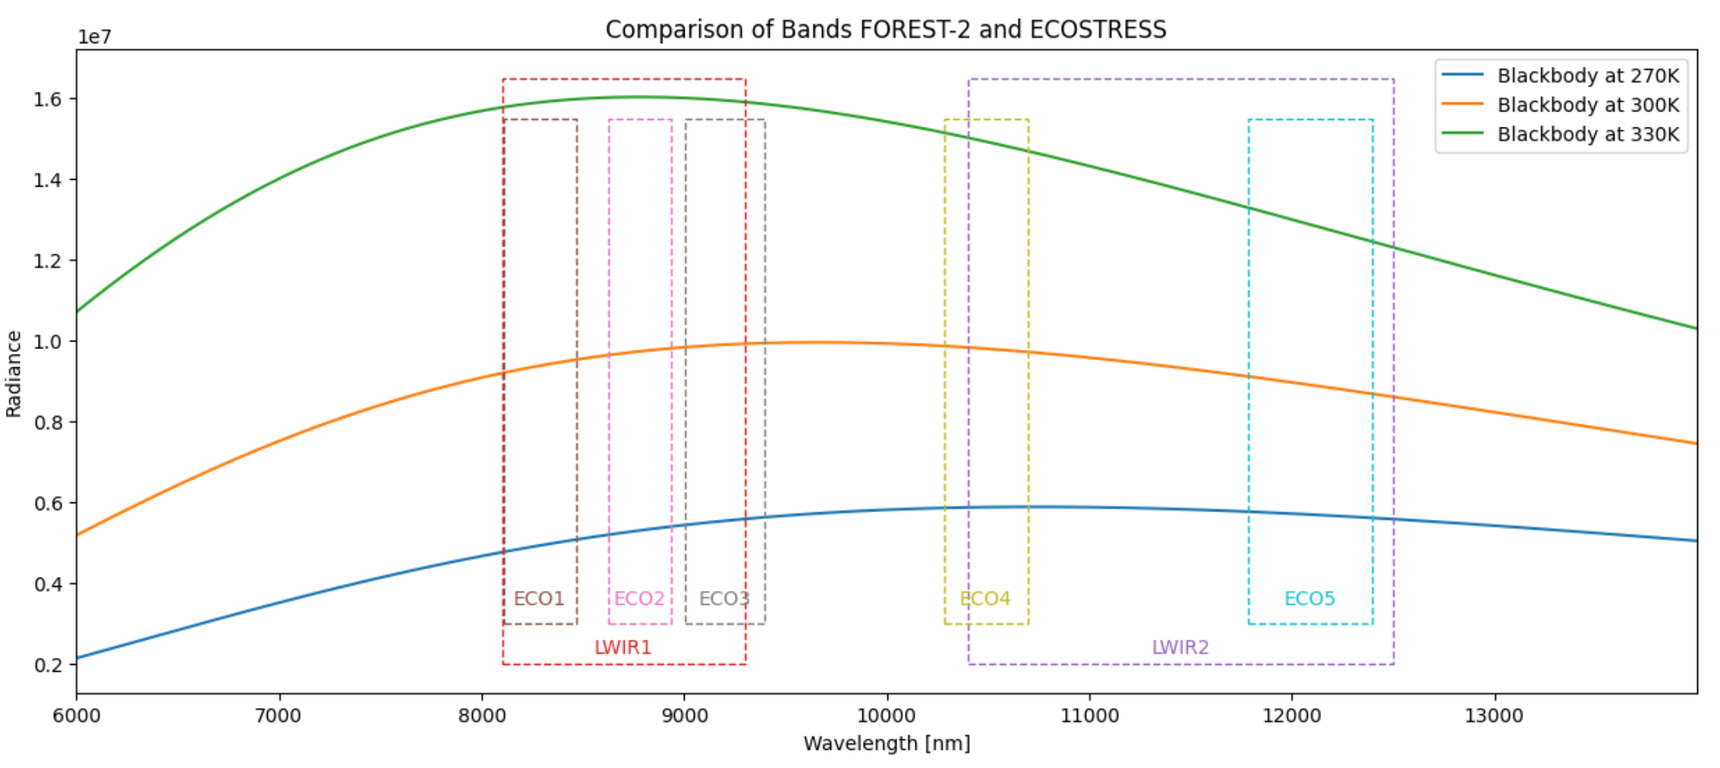
\includegraphics[width=\linewidth]{Includes/5-wavelength-comparison.png}
    \caption{Wavelengths of the sensors in ECOSTRESS and FOREST satellites. The radiation spectrum of black bodies at different temperatures is included for comparison.}
    \label{fig:5-wavelength-comparison}
\end{figure}

\subsubsection{Accessing ECOSTRESS Scenes}
    ECOSTRESS imagery is available via NASA's Application for Extracting and Exploring Analysis Ready Samples (AppEEARS) \cite{AppEEARS2023}. This tool allows the request of area samples via vector polygons. Using the product's API \cite{AppEEARSAPI2023}, Level 1 Mapped Radiance scenes of size 200x200 km with center on the locations provided in Fig. \ref{fig:5-wavelength-comparison} were programmatically requested. Due to satellite hardware anomalies, certain spectral bands experienced acquisition gaps, needing a careful selection of date ranges to ensure the availability of all five bands \cite{ECO1BMAPRAD2023}.

   \begin{table}[h!]
        \centering
        \begin{tabular}{|l|l|}
        \hline
        Area     & 200 x 200 km                                                                              \\ \hline
        Products & \begin{tabular}[c]{@{}l@{}}Mapped Radiance (5 bands)\\ Quality (5 Bands)\end{tabular}     \\ \hline
        Dates    & \begin{tabular}[c]{@{}l@{}}2018/08/20 - 2019/03/04\\ 2023/05/01 - 2023/08/15\end{tabular} \\ \hline
        \end{tabular}
        \caption{Requests configuration}
        \label{tab:5-scenes-characteristics}
    \end{table}

    \begin{figure}[h!]
        \centering
        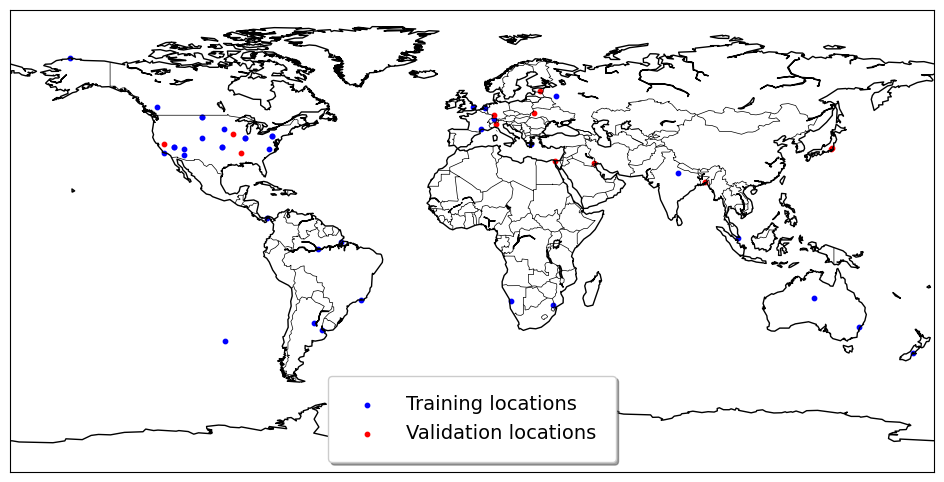
\includegraphics[width=\linewidth]{Includes/5-ecostress-map-location.png}
        \caption{Location of the samples taken from ecostress.}
        \label{fig:5-ecostress-map-location}
    \end{figure}

\subsubsection{Selecting the best scenes}

The AppEEARS platform returns multiple scenes that correspond to the specified area sample within the requested timeframe. This includes five mapped radiance measurements alongside their corresponding Quality Assurance (QA) bands. Additionally, a CSV file detailing quality statistics for each scene is provided. 

The interface returns any scene that overlaps with the requested area. For that reason, some GeoTIFFs may be significantly smaller than others, with variations reaching 90\%. Moreover, an important number of these GeoTIFFs may contain a high percentage of bad-quality pixels, rendering them unsuitable for model training. Furthermore, as highlighted in the ECOSTRESS frequently asked questions \cite{ecostress_faq}, the accuracy of radiance measurements is highly dependent on clear sky conditions; cloudy scenes typically yield negligible radiance emissions.

Downloading the entirety of the dataset is impractical due to its vast size.  
From the 50 scenes, each one is potentially replicated over 20 times over the ten-month request window.
Such a dataset, given its magnitude, cannot be used for model training with the available hardware resources.
Therefore, a procedure is developed to identify and select the most appropriate scene for each month based on a predefined set of criteria:

\begin{enumerate}
\item Scenes should have a low proportion of bad-quality pixels.
\item Scenes should have a considerable size so that many crops can be taken from it.
\item As clouds imply low radiance values, clear sky scenes will have high radiance values.
\end{enumerate}


The procedure to get the best scene for each month is detailed below: 

\begin{algorithm}
\caption{Process applied to the scenes returned from one area request.}
\begin{algorithmic}[1]

\State \textbf{QA statistics:}
\State Get the average proportion of good pixels $p_{gp}$ for the 5 radiances of the scene.
\State Discard scenes where $p_{gp} < 0.6 $ .

\State \textbf{Scene Statistics:}
\State Get the biggest scene of each month for each requested area.
\State Calculate the proportion between the size of each scene and the biggest of the month.
\State Discard images whose size proportion is smaller than 0.2.
\State Calculate the median of the radiance values of the scene.
\State \textbf{Selecting the scene of the month:}
\State Merge the QA statistics and the Scene statistics.
\State For each month, get the three scenes with the greatest $p_{gp}$.
\State Select the scene that has the greatest median radiance value.
\end{algorithmic}
\end{algorithm}

Applying this procedure, a dataset comprised of 5031 scenes taken from 50 area requests is reduced to 379 scenes.

\subsubsection{Data Processing}

In order to be able to use the data in a super-resolution algorithm, a set of processing steps must be performed on it.

The diagram in Fig. \ref{fig:5-data_processing_flow_chart} displays the processing pipeline. The inputs are the 5 Mapped radiance and their respective quality bands.

Mapped radiances 1,2 and 3 are averaged to form the LWIR1 synthetic FOREST, and mapped radiances 4 and 5 are averaged to form the LWIR2 synthetic FOREST. If any of the bands are missing, the corresponding LWIR synthetic forest is discarded. 

The fill values in the mapped radiances and the data quality classes are used to create a binary mask for each spectral band. If a pixel is considered problematic, it is marked as a 1 in the binary mask. The QA band for a synthetic FOREST LWIR band is built using an OR operation on the corresponding ECOSTRESS bands involved in its construction. After being constructed, both the synthetic LWIR and the corresponding QA band are reprojected to the most suitable UTM EPSG code based on the latitude and longitude of the scene.

\begin{table}[h!]
    \centering
    
    \label{tab:quality_classes}
    \begin{tabular}{cl}
        \toprule
        \textbf{Value} & \textbf{Description}                \\
        \midrule
        \multicolumn{2}{c}{Fill Value Classes}                \\
        -9997          & Pixel not seen                       \\
        -9998          & Missing data due to striping (not filled in) \\
        -9999          & Missing/bad data                     \\
        \midrule
        \multicolumn{2}{c}{Data Quality Classes}              \\
        0              & Good                                 \\
        1              & Missing stripe data, filled in       \\
        2              & Missing stripe data, not filled in   \\
        3              & Missing/bad data                     \\
        4              & Not seen                             \\
        \bottomrule
    \end{tabular}
    \caption{Fill Value and Data Quality Classes}
\end{table}

The synthetic LWIR images are not suitable for the super-resolution task yet.
They are too big to be kept in memory, and not all their values are of good quality.
For that reason, for each scene, a number of random crops of size 264x264 pixels are taken.
The random crop processor pipeline is displayed in Fig. \ref{fig:5-random_crop_processor}.
It is an iterative process where, at each stage, crops that do not comply with the quality considerations ( all pixels are of good quality, and no stripe noise was detected) are discarded until the target number of crops per scene is achieved.
Additionally, the Affine Transformation is translated so that the images can be georeferenced.


\begin{figure}[H]
    \centering
    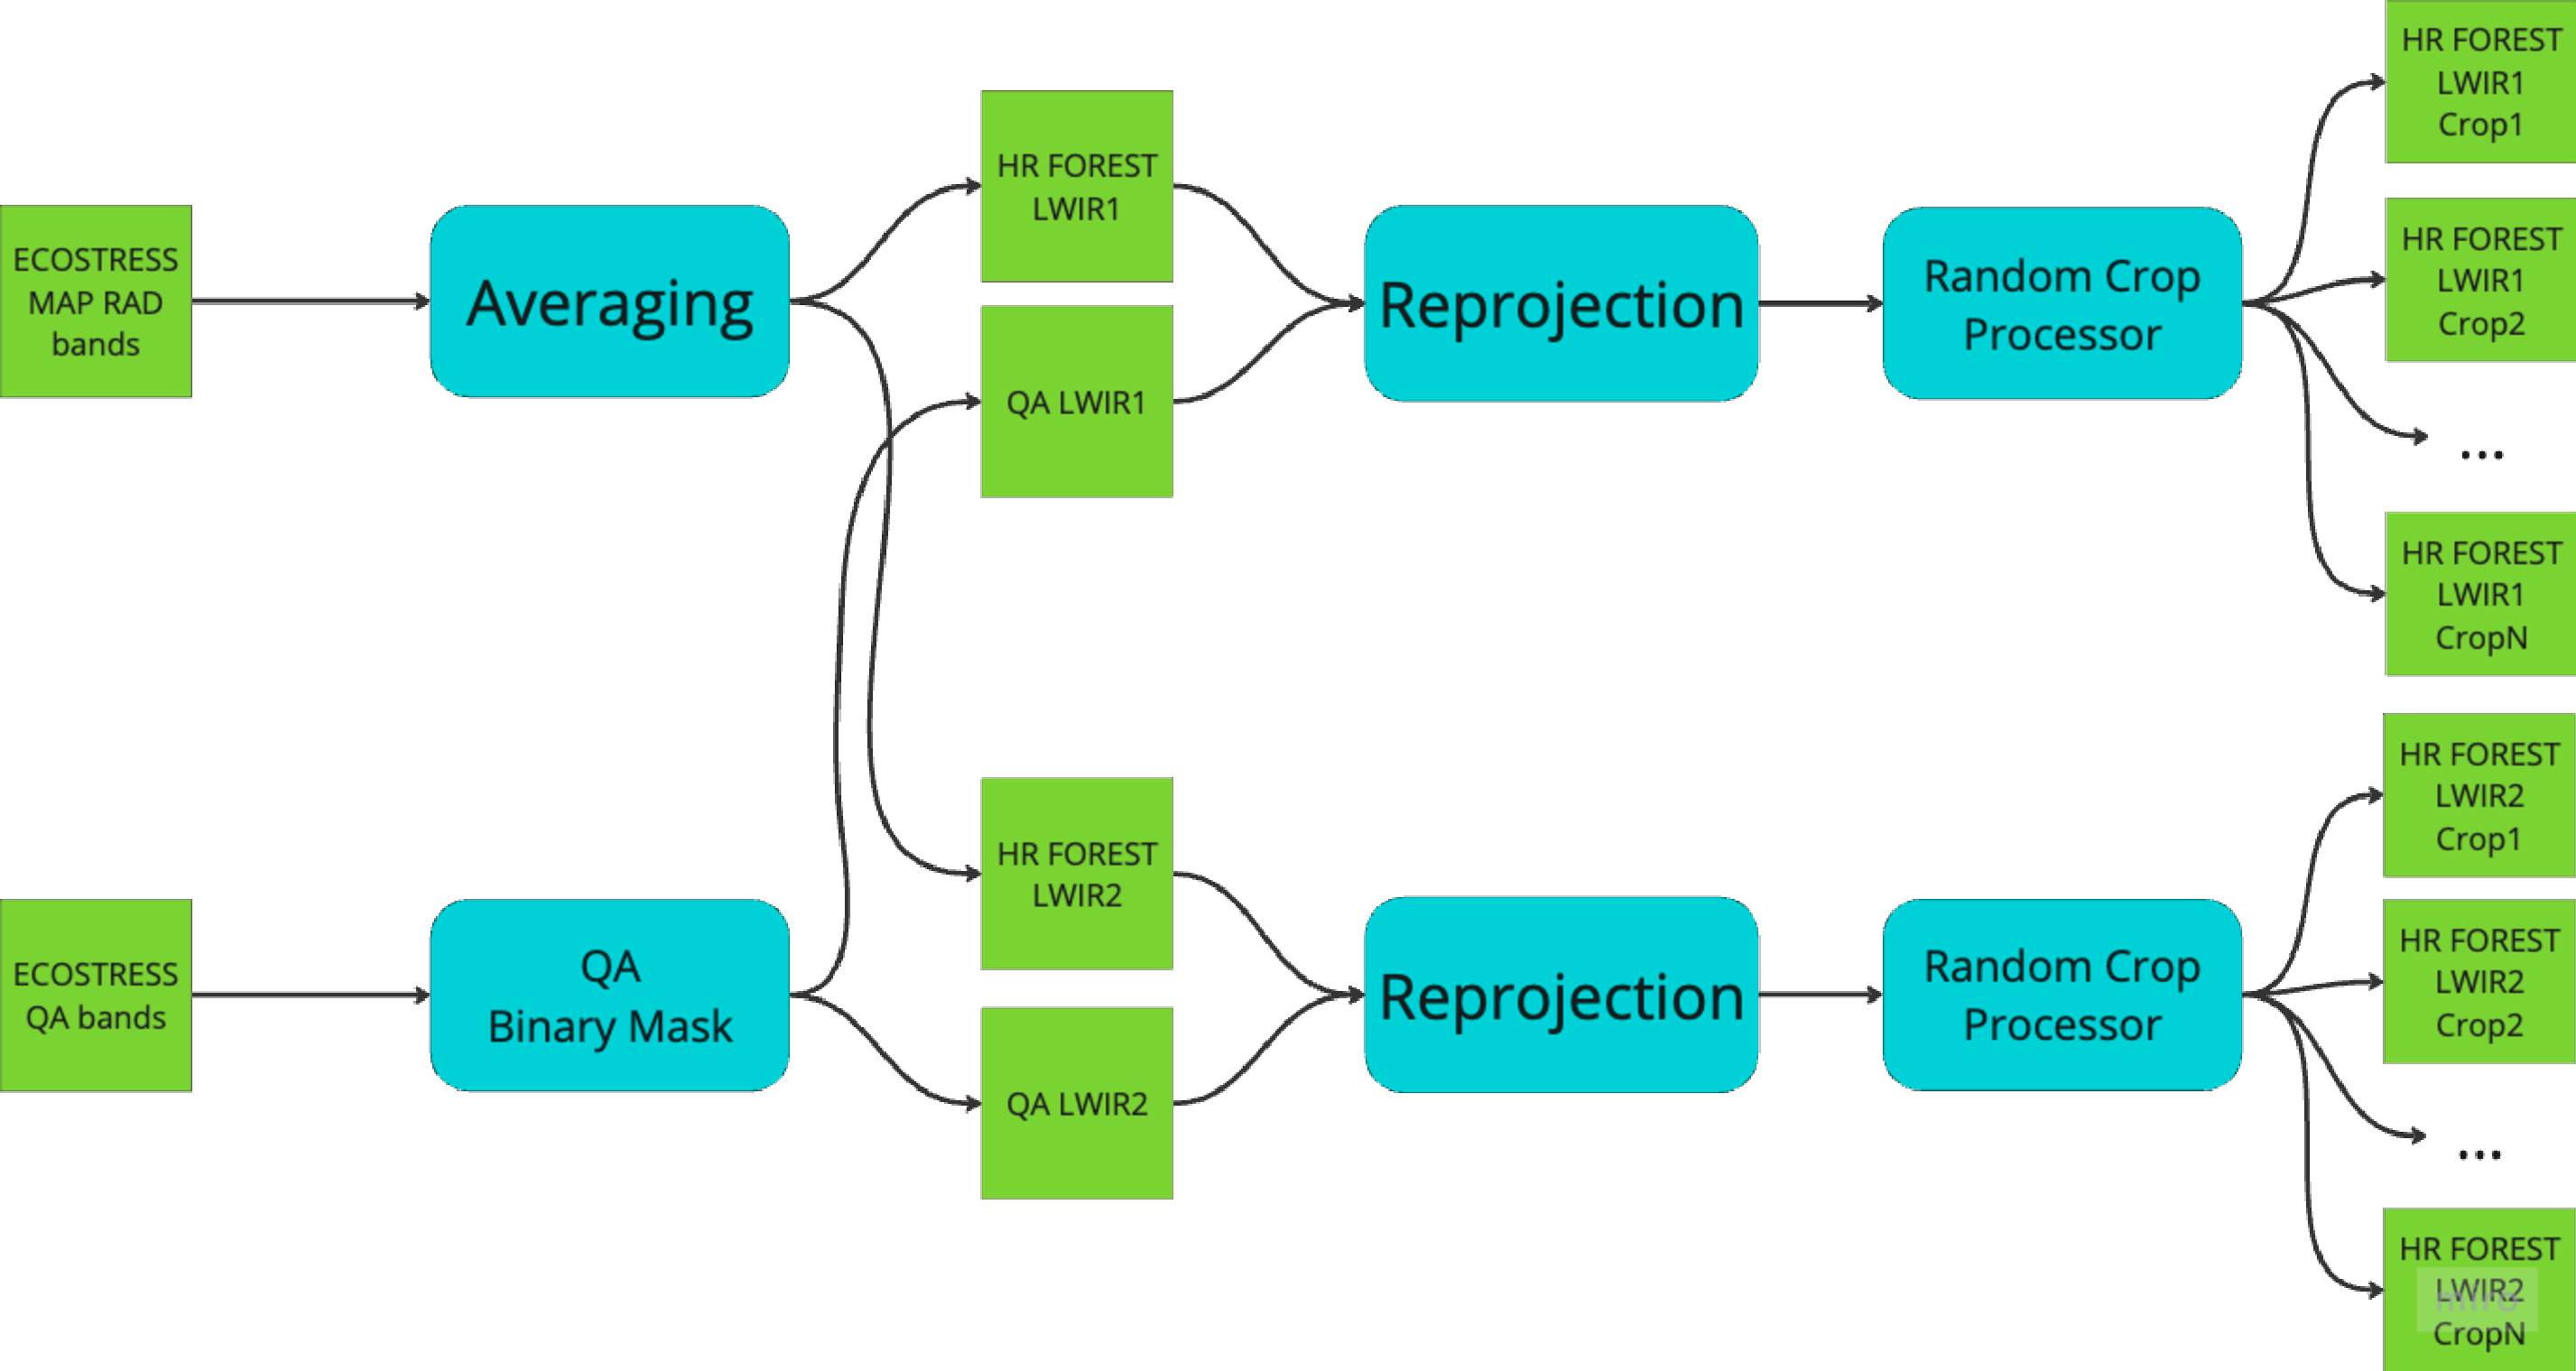
\includegraphics[width=\linewidth]{Includes/5-data_processing_flow_chart.pdf}
    \caption{Data processing workflow}
    \label{fig:5-data_processing_flow_chart}
\end{figure}

\begin{figure}[H]
    \centering
    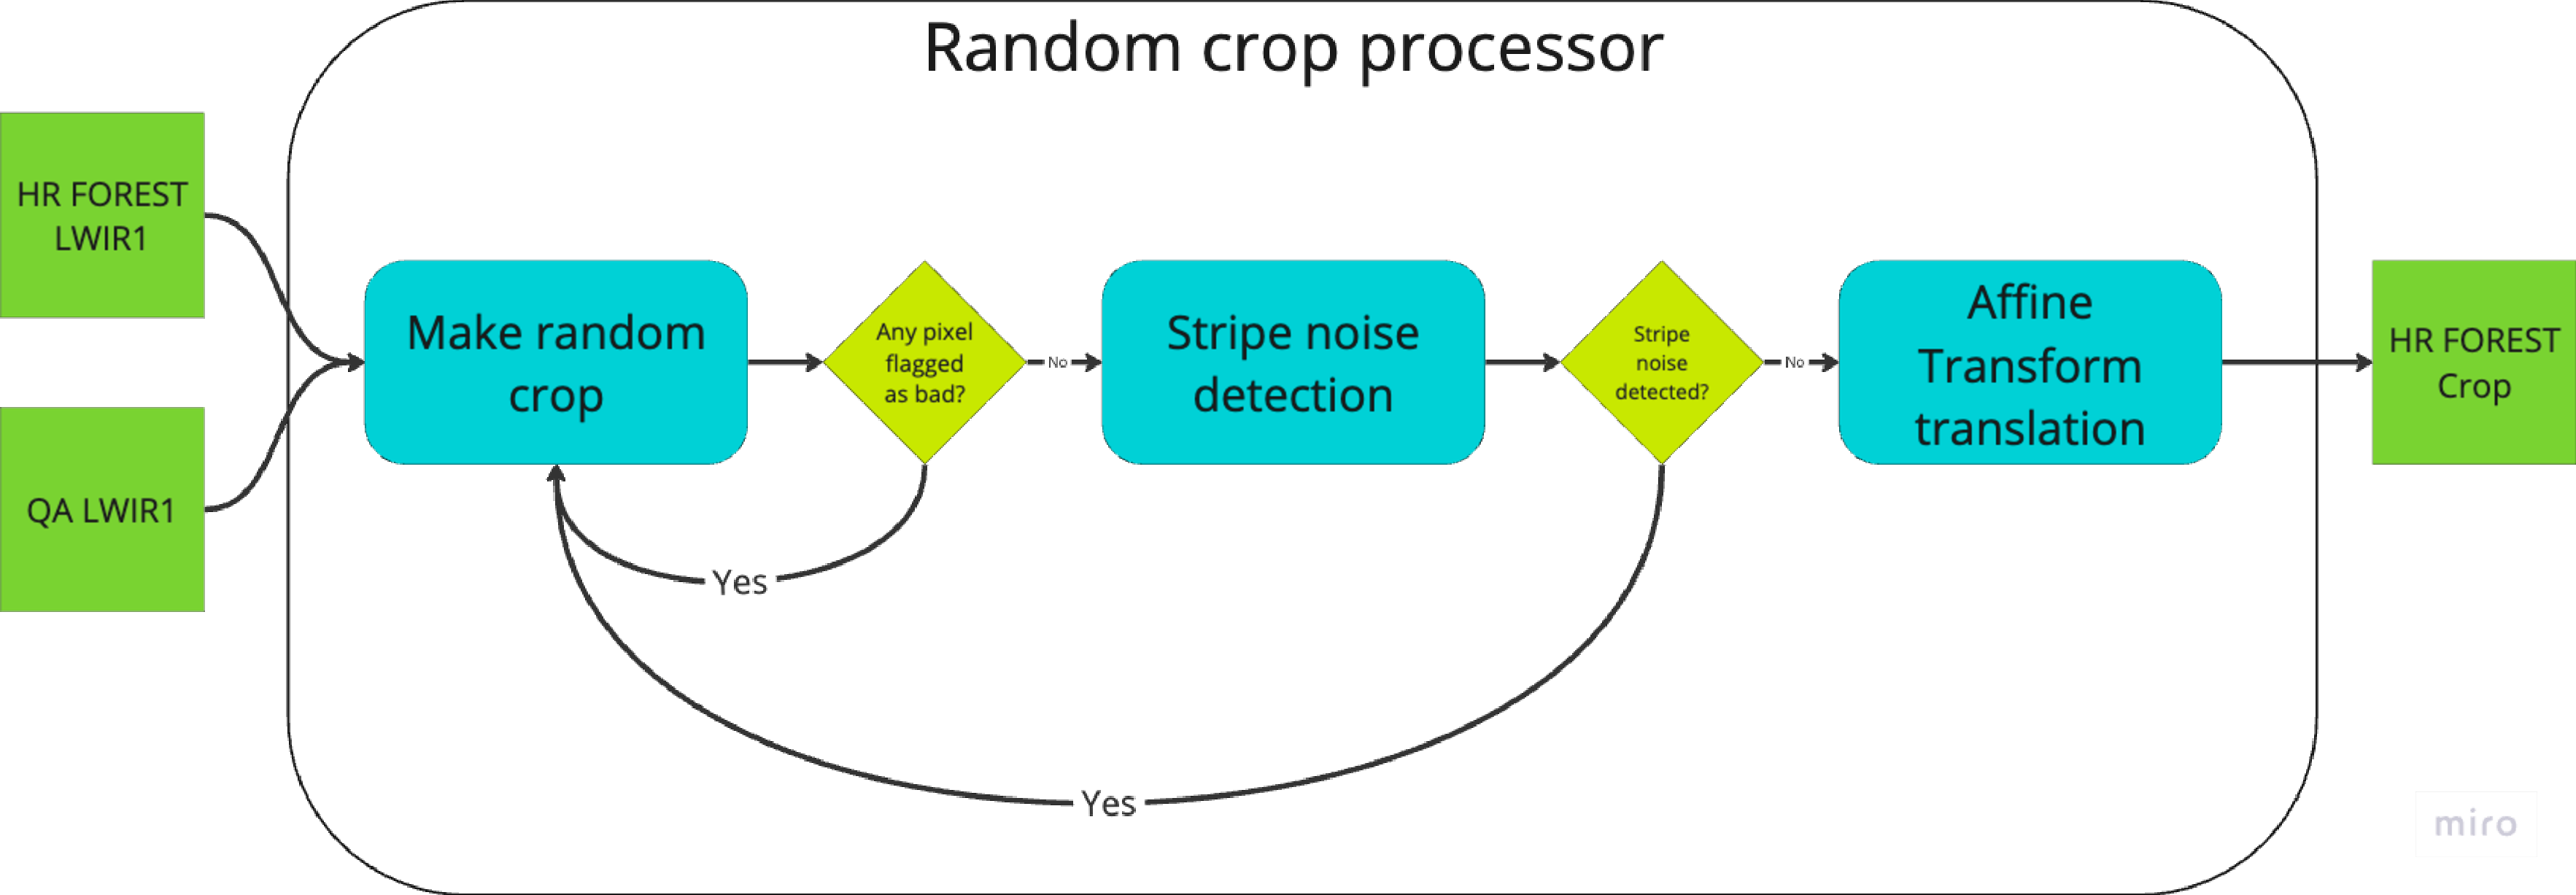
\includegraphics[width=\linewidth]{Includes/5-random_crop_processor.pdf}
    \caption{Random crop processor}
    \label{fig:5-random_crop_processor}
\end{figure}



\subsection{Obtaining FOREST-2 data}

    To obtain a dataset of FOREST-2 images, the company provides an internal API that allows the download of scenes captured by the satellite. 
    The download of the scenes is done programmatically in the locations provided in Fig. \ref{fig:4-forest-locations}. 

    \begin{figure}[H]
        \centering
        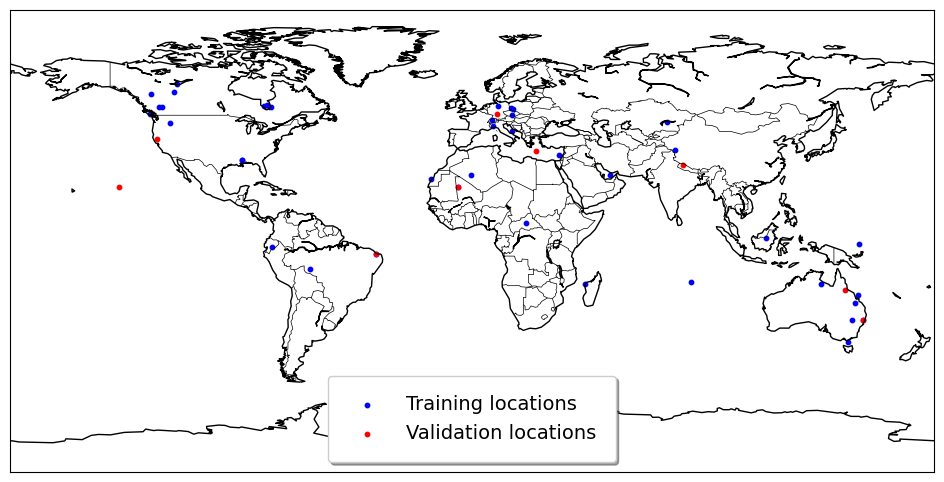
\includegraphics[width=\linewidth]{Includes/4-forest-locations.png}
        \caption{Location of the FOREST-2 scenes.}
        \label{fig:4-forest-locations}
    \end{figure}

    The scenes are downloaded in the NetCDF-4 format, containing the LWIR1, LWIR2, and MWIR bands, as well as the latitude and longitude information. 
    An example of a scene is shown in Fig. \ref{fig:4-forest-complete example}. 
    As in this work, the focus is on the long wave infra-red; the MWIR band is discarded.

    \begin{figure}[H]
        \centering
        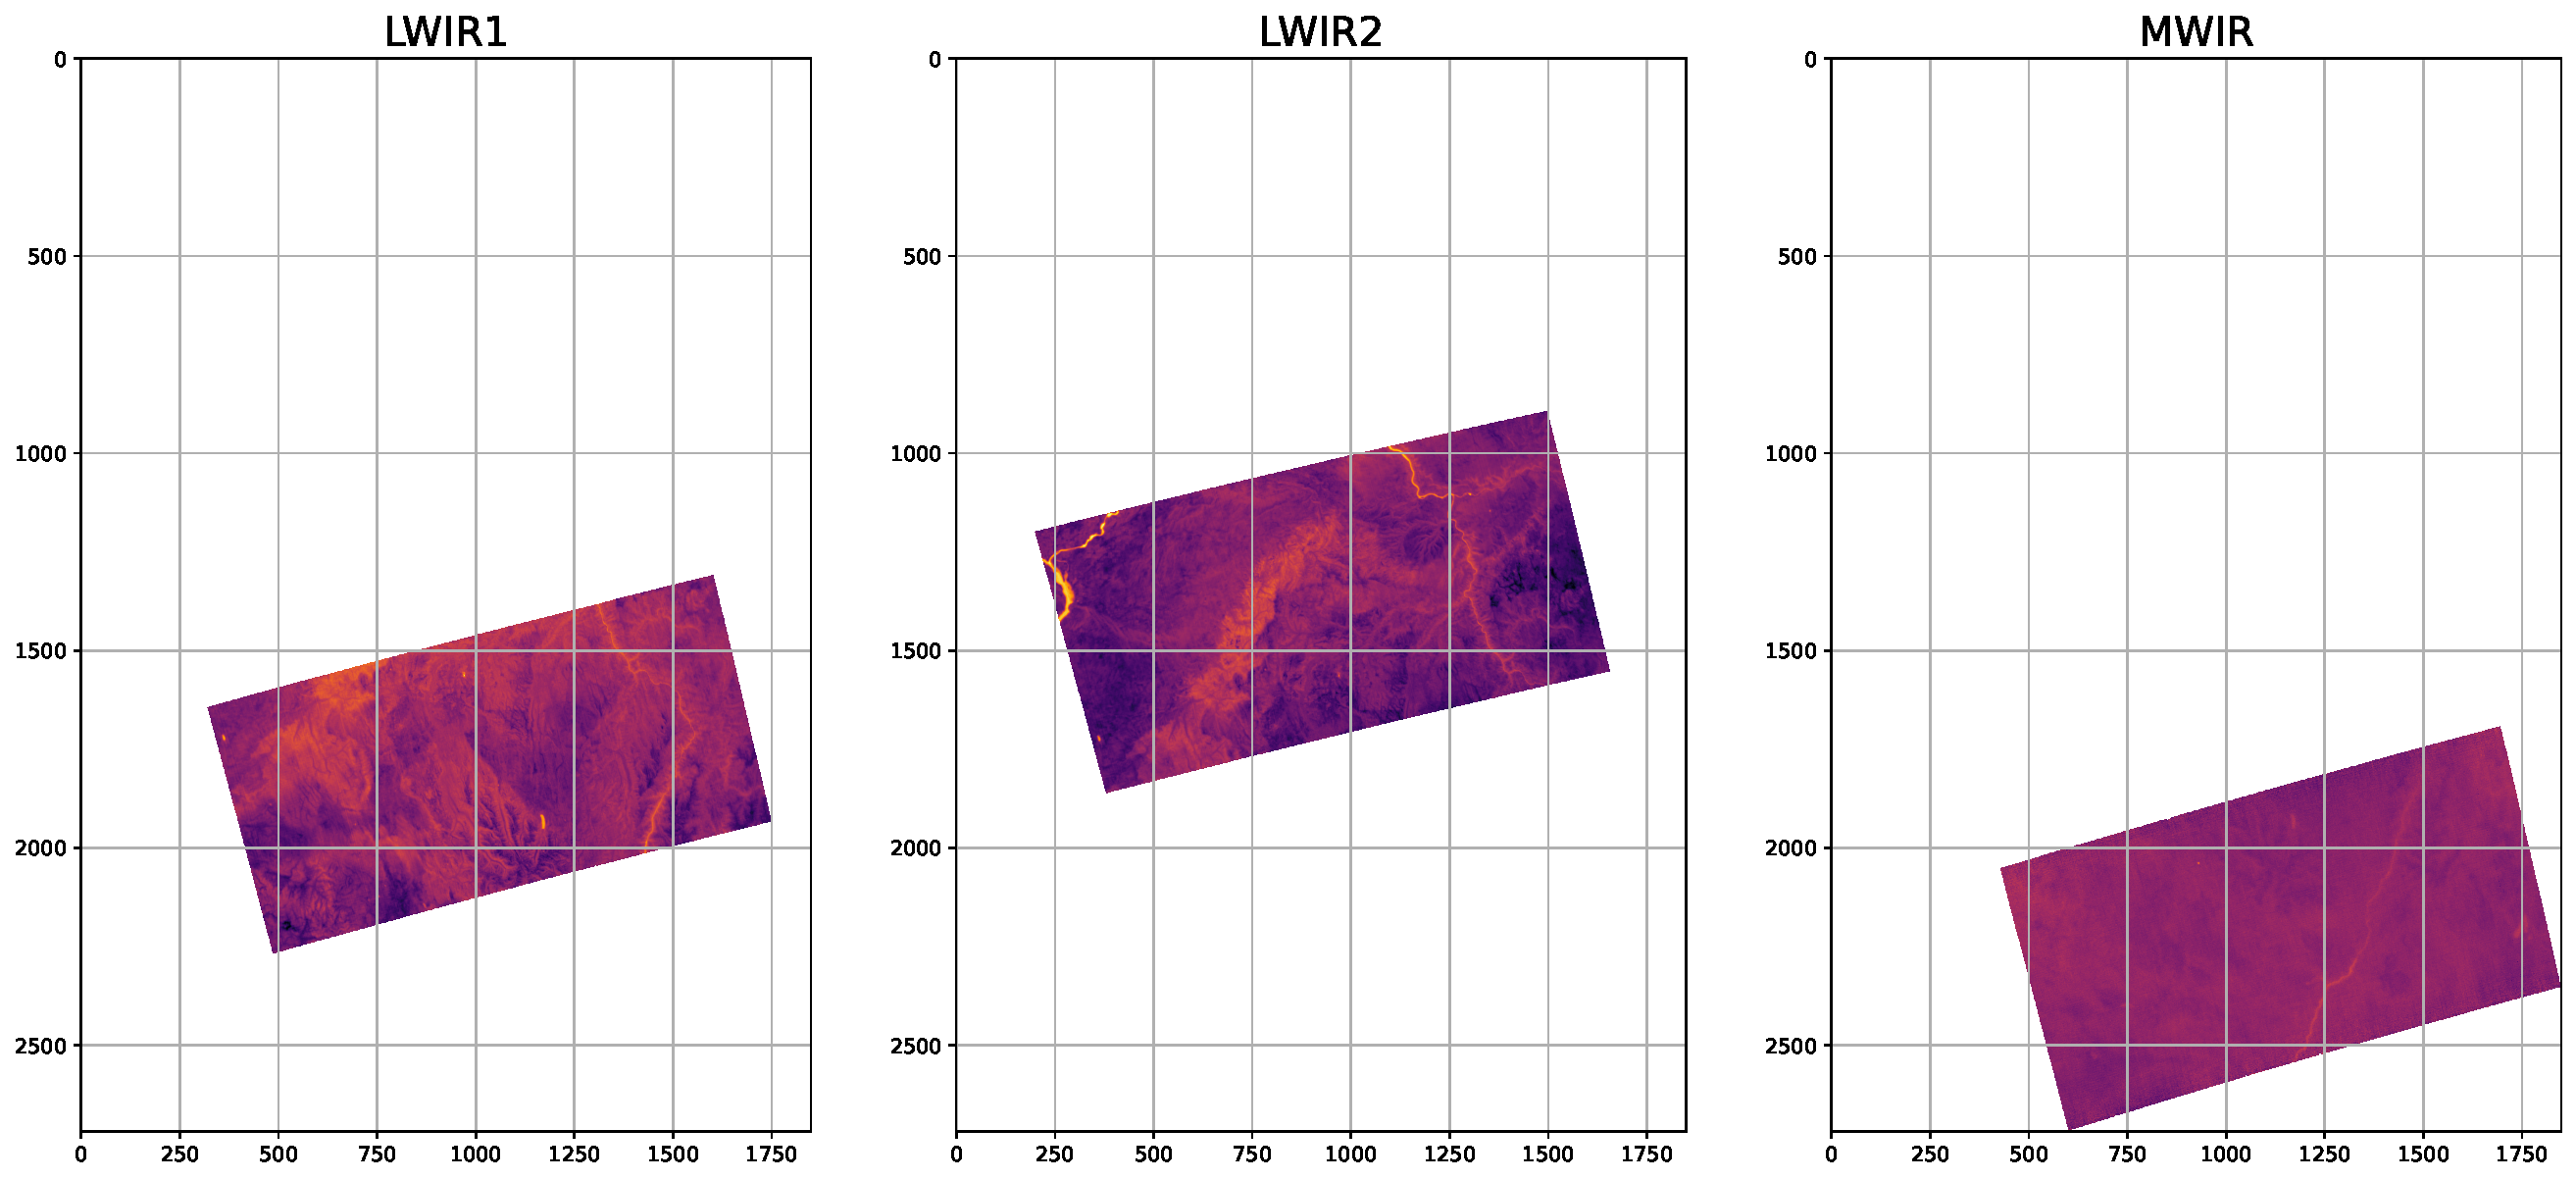
\includegraphics[width=\linewidth]{Includes/4-forest2-unprocessed-bands.pdf}
        \caption{LWIR1, LWIR2, and MWIR bands of a FOREST-2 scene downloaded from the company's API.}
        \label{fig:4-forest-complete example}
    \end{figure}

    The provided arrays have an enormous proportion of NA values and are not suitable for taking crops.
    For that, a bounding box is defined for each band, removing most of the NA values. 
    The resulting scenes are shown in Fig. \ref{fig:4-forest-bounding-box}.

    \begin{figure}[H]
        \centering
        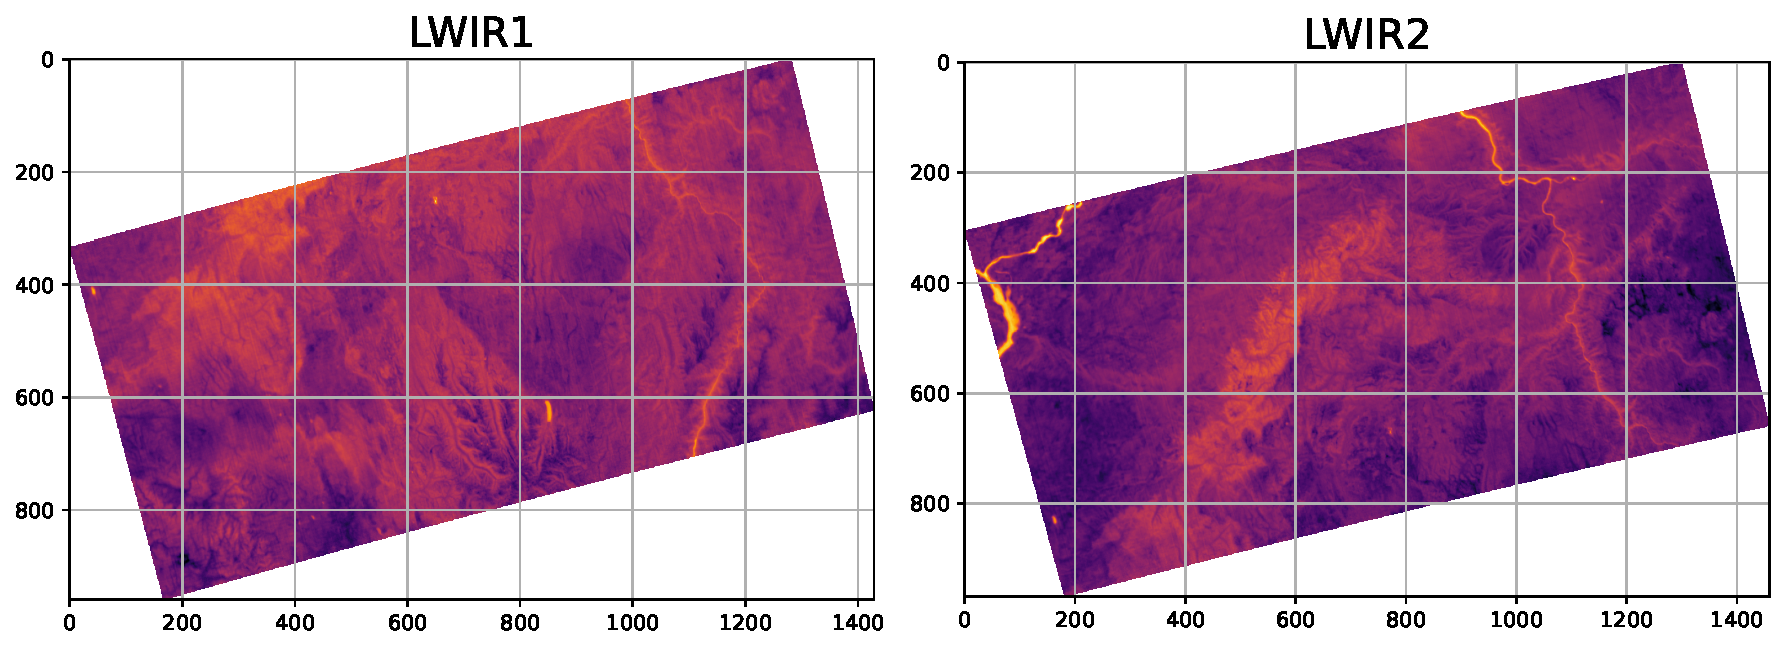
\includegraphics[width=\linewidth]{Includes/4-forest2-cropped-bands.pdf}
        \caption{LWIR1 and LWIR2 of a FOREST-2 scene downloaded from the company's API, after cropping NA values.}
        \label{fig:4-forest-bounding-box}
    \end{figure}

    A similar random crop processor as in Fig. \ref{fig:5-random_crop_processor} is used afterward. 
    The objective is to obtain several crops of size 88x88 pixels that match the 264x264 pixels of the synthetic HR FOREST-2 images when upscaled by a factor of 3.
    If any crop has any NA value or strip noise detected, it is discarded, and the process restarts, with a maximum retries of 100.
    Using the latitude and the longitude information, the affine transformation is calculated so that the crops can be georeferenced, if necessary.
    
\subsection{Datasets}

Several dataset combinations are used to better understand how the proposed architecture works. 
The implemented Pytorch dataset class loads and yields samples from two different file locations, one for the HR images (source domain) and one for the LR images (target domain). 
The source domain is the synthetic FOREST-2 images produced from ECOSTRESS, while the target domain is composed of LR images coming from different sources.
The samples are usually unpaired, meaning that the scenes are not compared on an image-to-image basis. Still, the implementation allows the use of paired datasets in order to calculate supervised metrics. 
In case any of the domains has less samples than the other, the class will bootstrap it to match the size of the other.



% % Please add the following required packages to your document preamble:
% % \usepackage{graphicx}
% \begin{table}[H]
%     \centering
%     \resizebox{\textwidth}{!}{%
%     \begin{tabular}{c|cccc|cccc|cccc}
%                 & \multicolumn{4}{c|}{$\mathcal{D}_{\text{SF}-\text{SF}}$}                                                                                                                                                                                                                                           & \multicolumn{4}{c|}{$\mathcal{D}_{\text{SF}-\text{RF}}$}                                                                                                                                                                                                 & \multicolumn{4}{c|}{$\mathcal{D}_{\text{SF}-\text{RF}}^{\text{Paired}}$}                                                                                                                                                                                                      \\ \cline{2-13} 
%                 & \multicolumn{2}{c|}{Training}                                                                                                                                         & \multicolumn{2}{c|}{Validation}                                                                                            & \multicolumn{2}{c|}{Training}                                                                                                         & \multicolumn{2}{c|}{Validation}                                                                                  & \multicolumn{2}{c|}{Training}                                                                                                         & \multicolumn{2}{c|}{Validation}                                                                                                       \\
%                 & \multicolumn{1}{c|}{Source}                                                  & \multicolumn{1}{c|}{Target}                                                            & source                                                 & target                                                            & source                                                 & \multicolumn{1}{c|}{target}                                                  & source                                                 & target                                                  & source                                                 & \multicolumn{1}{c|}{target}                                                  & source                                                 & \multicolumn{1}{c|}{target}                                                  \\ \hline
%     Image       & \multicolumn{1}{c|}{\begin{tabular}[c]{@{}c@{}}Synth \\ FOREST\end{tabular}} & \multicolumn{1}{c|}{\begin{tabular}[c]{@{}c@{}}Degraded\\ synth\\ FOREST\end{tabular}} & \begin{tabular}[c]{@{}c@{}}Synth\\ FOREST\end{tabular} & \begin{tabular}[c]{@{}c@{}}Degraded\\ synth\\ FOREST\end{tabular} & \begin{tabular}[c]{@{}c@{}}Synth\\ FOREST\end{tabular} & \multicolumn{1}{c|}{\begin{tabular}[c]{@{}c@{}}Real\\ FOREST-2\end{tabular}} & \begin{tabular}[c]{@{}c@{}}Synth\\ FOREST\end{tabular} & \begin{tabular}[c]{@{}c@{}}Real\\ FOREST-2\end{tabular} & \begin{tabular}[c]{@{}c@{}}Synth\\ FOREST\end{tabular} & \multicolumn{1}{c|}{\begin{tabular}[c]{@{}c@{}}Real\\ FOREST-2\end{tabular}} & \begin{tabular}[c]{@{}c@{}}Synth\\ FOREST\end{tabular} & \multicolumn{1}{c|}{\begin{tabular}[c]{@{}c@{}}Real\\ FOREST-2\end{tabular}} \\ \hline
%     n           & \multicolumn{1}{c|}{13764}                                                   & \multicolumn{1}{c|}{13764}                                                             & 2676                                                   & 2676                                                              & 13764                                                  & \multicolumn{1}{c|}{4000}                                                    & 2676                                                   & 1200                                                    & 13764                                                  & \multicolumn{1}{c|}{4000}                                                    & ??                                                     & \multicolumn{1}{c|}{??}                                                      \\ \hline
%     scale ratio & \multicolumn{1}{c|}{x3}                                                      & \multicolumn{1}{c|}{x3}                                                                & x3                                                     & x3                                                                & x3                                                     & \multicolumn{1}{c|}{x3}                                                      & x3                                                     & x3                                                      & x3                                                     & \multicolumn{1}{c|}{x3}                                                      & x3                                                     & \multicolumn{1}{c|}{x3}                                                      \\ \hline
%     crop size   & \multicolumn{1}{c|}{264}                                                     & \multicolumn{1}{c|}{88}                                                                & 264                                                    & 88                                                                & 264                                                    & \multicolumn{1}{c|}{88}                                                      & 792                                                    & 264                                                     & 264                                                    & \multicolumn{1}{c|}{88}                                                      & ??                                                     & \multicolumn{1}{c|}{??}                                                      \\ \hline
%     Paired?     & \multicolumn{2}{c|}{No}                                                                                                                                               & \multicolumn{2}{c|}{Yes}                                                                                                   & \multicolumn{2}{c|}{No}                                                                                                               & \multicolumn{2}{c|}{No}                                                                                          & \multicolumn{2}{c|}{No}                                                                                                               & \multicolumn{2}{c}{Yes}                                                                                                               \\ \hline
%                 & \multicolumn{1}{c|}{}                                                        & \multicolumn{1}{c|}{}                                                                  &                                                        &                                                                   &                                                        & \multicolumn{1}{c|}{}                                                        &                                                        &                                                         &                                                        & \multicolumn{1}{c|}{}                                                        &                                                        & \multicolumn{1}{c|}{}                                                        \\ \hline
%                 & \multicolumn{1}{c|}{}                                                        & \multicolumn{1}{c|}{}                                                                  &                                                        &                                                                   &                                                        & \multicolumn{1}{c|}{}                                                        &                                                        &                                                         &                                                        & \multicolumn{1}{c|}{}                                                        &                                                        & \multicolumn{1}{c|}{}                                                        \\ \hline
%                 & \multicolumn{1}{c|}{}                                                        & \multicolumn{1}{c|}{}                                                                  &                                                        &                                                                   &                                                        & \multicolumn{1}{c|}{}                                                        &                                                        &                                                         &                                                        & \multicolumn{1}{c|}{}                                                        &                                                        & \multicolumn{1}{c|}{}                                                        \\ \hline
%                 & \multicolumn{1}{c|}{}                                                        & \multicolumn{1}{c|}{}                                                                  &                                                        &                                                                   &                                                        & \multicolumn{1}{c|}{}                                                        &                                                        &                                                         &                                                        & \multicolumn{1}{c|}{}                                                        &                                                        & \multicolumn{1}{c|}{}                                                        \\ \hline
%                 & \multicolumn{1}{c|}{}                                                        & \multicolumn{1}{c|}{}                                                                  &                                                        &                                                                   &                                                        & \multicolumn{1}{c|}{}                                                        &                                                        &                                                         &                                                        & \multicolumn{1}{c|}{}                                                        &                                                        & \multicolumn{1}{c|}{}                                                       
%     \end{tabular}%
%     }
%     \caption{}
%     \label{tab:my-table}
%     \end{table}

% Please add the following required packages to your document preamble:
% \usepackage{graphicx}
\begin{table}[H]
    \centering
    \resizebox{\textwidth}{!}{%
    \begin{tabular}{|c|cccc|cccc|}
    \hline
                & \multicolumn{4}{c|}{$\mathcal{D}_{\text{SF}-\text{SF}}$}                                                                                                                                                                                                                                         & \multicolumn{4}{c|}{$\mathcal{D}_{\text{SF}-\text{RF}}$}                                                                                                                                                                                                               \\
                & \multicolumn{2}{c|}{Training}                                                                                                                             & \multicolumn{2}{c|}{Validation}                                                                                                      & \multicolumn{2}{c|}{Training}                                                                                                                & \multicolumn{2}{c|}{Validation}                                                                                         \\ \hline
    Domain      & Source                                                       & \multicolumn{1}{c|}{Target}                                                                & Source                                                       & Target                                                                & Source                                                       & \multicolumn{1}{c|}{Target}                                                   & Source                                                       & Target                                                   \\ \hline
    Image type      & \begin{tabular}[c]{@{}c@{}}Synth HR \\ FOREST-2\end{tabular} & \multicolumn{1}{c|}{\begin{tabular}[c]{@{}c@{}}Degraded Synth \\ HR FOREST-2\end{tabular}} & \begin{tabular}[c]{@{}c@{}}Synth HR \\ FOREST-2\end{tabular} & \begin{tabular}[c]{@{}c@{}}Degraded Synth\\  HR FOREST-2\end{tabular} & \begin{tabular}[c]{@{}c@{}}Synth HR\\  FOREST-2\end{tabular} & \multicolumn{1}{c|}{\begin{tabular}[c]{@{}c@{}}Real \\ FOREST-2\end{tabular}} & \begin{tabular}[c]{@{}c@{}}Synth HR\\  FOREST-2\end{tabular} & \begin{tabular}[c]{@{}c@{}}Real\\  FOREST-2\end{tabular} \\ \hline
    Crop number & 13764                                                        & \multicolumn{1}{c|}{13764}                                                                 & 2676                                                         & 2676                                                                  & 13764                                                        & \multicolumn{1}{c|}{4000}                                                     & 2676                                                         & 1200                                                     \\ \hline
    Crop size   & 264                                                          & \multicolumn{1}{c|}{88}                                                                    & 264                                                          & 88                                                                    & 264                                                          & \multicolumn{1}{c|}{88}                                                       & 792                                                          & 264                                                      \\ \hline
    Scale ratio & 3                                                            & \multicolumn{1}{c|}{3}                                                                     & 3                                                            & 3                                                                     & 3                                                            & \multicolumn{1}{c|}{3}                                                        & 3                                                            & 3                                                        \\ \hline
    Paired?     & \multicolumn{2}{c|}{No}                                                                                                                                   & \multicolumn{2}{c|}{Yes}                                                                                                             & \multicolumn{2}{c|}{No}                                                                                                                      & \multicolumn{2}{c|}{No}                                                                                                 \\ \hline
    \end{tabular}%
    }
    \caption{Dataset characteristics}
    \label{tab:dataset_characteristics}
    \end{table}


\subsubsection{Synthetic FOREST - Degraded Synthetic FOREST}
    The dataset $\mathcal{D}_{\text{SF}-\text{SF}}$ is built by taking the HR synthetic FOREST crops and applying the baseline degradation model proposed in \ref{subsec:baseline_degradation_model}. 
    The 264x264 crops are reduced to 88x88. The training set is used to train the SR model, while the validation set is used to monitor the training process and avoid overfitting. 
    Even though, in this case, the HR and LR versions of the same scene are available, the training dataset is unpaired by shuffling the samples.
    The validation set is not shuffled, and thus, metrics like PSNR and SSIM can be calculated in the target domain. The parameters used for the degradation model are described below:

    \begin{table}[H]
        \centering
        \begin{tabular}{l|l}
        Parameter & Value \\ \hline
        downscaling ratio & 3 \\ 
        Gaussian Kernel size & 21 \\ 
        Gaussian kernel sigma in X axis &  $\sim \mathcal{N}(1,0.3)$  \\ 
        Gaussian kernel sigma in Y axis &  $\sim \mathcal{N}(1,0.3)$  \\ 
        target radiometric error & 1.5K \\ 
        white noise factor & 0.5 \\ 
        constant noise factor & 0.5 \\ 
        \end{tabular}
        \caption{Parameters used in the degradation model employed to generate the $\mathcal{D}_{\text{SF}-\text{SF}}$ dataset.}
        \label{tab:degradation_model_parameters}
    \end{table}

\subsubsection{Synthetic FOREST - real FOREST (Unpaired)}
    The dataset $\mathcal{D}_{\text{SF}-\text{RF}}$ is composed of the 264x264 synthetic HR FOREST-2 crops as the source domain and  88x88 real FOREST-2 crops as the target domain. 
    The validation dataset is not paired, as the HR and LR images are entirely different scenes.
    Thus, supervised metrics are not available for the super-resolved target domain images. 
    The metric used to determine the best model is the PSNR from the super resolution of the output of the degradation model generator.

\subsubsection{Paired data acquisition} \label{subsec:pairedacquisition}

    When two missions pass over the same geographic region in a relatively similar timeframe, the overlap between their recorded scenes allows the collection of paired datasets. In order to do that with ECOSTRESS and FOREST-2, the trajectory of both missions is closely monitored to detect when they are close enough for data acquisition. As the intersection of the trajectories is not a perfect match, some processing must be done to co-register the images taken from both satellites. 

    In the case of ECOSTRESS and FOREST-2, paired data would be available once per week. However, because of issues in data quality from both missions or atmospheric factors such as cloud cover, only a single scene was successfully captured in the timeframe of this work. Although the amount of images is not sufficient to create a proper validation dataset, the scene will be used to assess the performance of the SR models. To avoid errors on the PSNR due to wrong co-registration of the images, the adjusted metrics explained in \ref{subsec:adjustedmetrics} will be used.




\newpage
\section{Experiment Setup}

The experiments were conducted using a single RTX 4090 GPU with 24GB of RAM. A condensed overview of the experiment setup is available in Table \ref{tab:experiment-setup}.

For the degradation model, the dimensions of $z_k$ and $z_n$ were set to $64$, using eight residual blocks as the core of both generative networks and a kernel size of $21$ for the kernel generator. Each pixel of the noise generator is correlated with its neighbors because the convolutional weights of the residual blocks have a size of 3x3. The discriminator is composed of 3 residual blocks, with 64 feature maps and a stride of 2 to create the patches.

The SR model is composed of 7 residual blocks, with 128 feature maps and an upsampling scale of 3. Compared to the original architecture, this one is more complex and has more parameters.

The adversarial loss used was the LSGAN loss, and the pixel-wise loss was the L1 loss. The noise regularization loss was the L2 norm of the noise output. The weights of the losses were set to 1 for the adversarial loss, 1 for the pixel-wise loss, and 100 for the noise regularization loss.

The models are trained sequentially during an epoch. First the generator, then the discriminator, and finally the SR model. Each network has its own ADAM optimizer, with a learning rate of $2 \cdot 10^{-4}$,
 $\beta_1 = 0.9$ and $\beta_2 = 0.99$. The discriminator is trained the same amount of times as the generator, as this was the ratio that produced the best results. The batch size was set to 16, and the number of epochs to 100. An instance normalization is performed on the dataset samples before going into the model.

The criteria to select the best model for each training session was the PSNR on the source domain of the validation set. 
In other words, the selected model is the one that achieved the highest PSNR after taking an HR image from the source domain, applying the probabilistic degradation model, then the SR model, and finally comparing the result with the original HR image.
This criterion depends heavily on monitoring the adversarial loss, as the overall network has two main objectives: fool the discriminator and generate a good SR image. If the adversarial loss is not monitored, the network could generate a good SR image at the cost of not doing a correct degradation. Moreover, the size of the discriminator was chosen so that it would always be a challenge for the generator to fool it.

\begin{table}[H]
    \centering
    \resizebox{\textwidth}{!}{%
    \begin{tabular}{|ccc|cc|}
    \hline
    \multicolumn{1}{|c|}{\multirow{19}{*}{Degradation Model}} & \multicolumn{1}{c|}{\multirow{14}{*}{Generator}}  & \multirow{7}{*}{Kernel} & Channels                     & 1                  \\
    \multicolumn{1}{|c|}{}                                    & \multicolumn{1}{c|}{}                             &                         & Feature maps                 & 64                 \\
    \multicolumn{1}{|c|}{}                                    & \multicolumn{1}{c|}{}                             &                         & Residual blocks              & 8                  \\
    \multicolumn{1}{|c|}{}                                    & \multicolumn{1}{c|}{}                             &                         & Kernel size                  & 21                 \\
    \multicolumn{1}{|c|}{}                                    & \multicolumn{1}{c|}{}                             &                         & LR image as input            & No                 \\
    \multicolumn{1}{|c|}{}                                    & \multicolumn{1}{c|}{}                             &                         & Pixel Invariant              & Yes                \\
    \multicolumn{1}{|c|}{}                                    & \multicolumn{1}{c|}{}                             &                         & Initialization               & Normal             \\ \cline{3-5} 
    \multicolumn{1}{|c|}{}                                    & \multicolumn{1}{c|}{}                             & \multirow{7}{*}{Noise}  & Channels                     & 1                  \\
    \multicolumn{1}{|c|}{}                                    & \multicolumn{1}{c|}{}                             &                         & Feature maps                 & 64                 \\
    \multicolumn{1}{|c|}{}                                    & \multicolumn{1}{c|}{}                             &                         & Residual blocks              & 8                  \\
    \multicolumn{1}{|c|}{}                                    & \multicolumn{1}{c|}{}                             &                         & LR image as input            & Yes                \\
    \multicolumn{1}{|c|}{}                                    & \multicolumn{1}{c|}{}                             &                         & Pixel Invariant              & No                 \\
    \multicolumn{1}{|c|}{}                                    & \multicolumn{1}{c|}{}                             &                         & Initialization               & Zero               \\
    \multicolumn{1}{|c|}{}                                    & \multicolumn{1}{c|}{}                             &                         & Conv weights size            & 3                  \\ \cline{2-5} 
    \multicolumn{1}{|c|}{}                                    & \multicolumn{2}{c|}{\multirow{5}{*}{Discriminator}}                         & Channels                     & 1                  \\
    \multicolumn{1}{|c|}{}                                    & \multicolumn{2}{c|}{}                                                       & Feature maps                 & 64                 \\
    \multicolumn{1}{|c|}{}                                    & \multicolumn{2}{c|}{}                                                       & Residual blocks              & 3                  \\
    \multicolumn{1}{|c|}{}                                    & \multicolumn{2}{c|}{}                                                       & Stride                       & 2                  \\
    \multicolumn{1}{|c|}{}                                    & \multicolumn{2}{c|}{}                                                       & Initialization               & Zero               \\ \hline
    \multicolumn{3}{|c|}{\multirow{4}{*}{SR model}}                                                                                         & Channels                     & 1                  \\
    \multicolumn{3}{|c|}{}                                                                                                                  & Feature maps                 & 128                \\
    \multicolumn{3}{|c|}{}                                                                                                                  & Residual Blocks              & 7                  \\
    \multicolumn{3}{|c|}{}                                                                                                                  & Upsampling scale             & 3                  \\ \hline
    \multicolumn{1}{|c|}{\multirow{7}{*}{Losses}}             & \multicolumn{2}{c|}{\multirow{2}{*}{Adversarial}}                           & Type                         & lsgan              \\
    \multicolumn{1}{|c|}{}                                    & \multicolumn{2}{c|}{}                                                       & weight                       & 1                  \\ \cline{2-5} 
    \multicolumn{1}{|c|}{}                                    & \multicolumn{2}{c|}{\multirow{3}{*}{Pixel wise}}                            & Type                         & L1                 \\
    \multicolumn{1}{|c|}{}                                    & \multicolumn{2}{c|}{}                                                       & Weight                       & 1                  \\
    \multicolumn{1}{|c|}{}                                    & \multicolumn{2}{c|}{}                                                       & Bias correction              & Yes                \\ \cline{2-5} 
    \multicolumn{1}{|c|}{}                                    & \multicolumn{2}{c|}{\multirow{2}{*}{Noise regularization}}                  & Type                         & L2 norm            \\
    \multicolumn{1}{|c|}{}                                    & \multicolumn{2}{c|}{}                                                       & Weight                       & 100                \\ \hline
    \multicolumn{1}{|c|}{\multirow{5}{*}{Optimizers}}         & \multicolumn{2}{c|}{\multirow{5}{*}{Same parameters for the three of them}} & Type                         & ADAM               \\
    \multicolumn{1}{|c|}{}                                    & \multicolumn{2}{c|}{}                                                       & Learning Rate                & $2 \cdot 10^{-4}$  \\
    \multicolumn{1}{|c|}{}                                    & \multicolumn{2}{c|}{}                                                       & $\beta_1$                    & 0.9                \\
    \multicolumn{1}{|c|}{}                                    & \multicolumn{2}{c|}{}                                                       & $\beta_2$                    & 0.99               \\
    \multicolumn{1}{|c|}{}                                    & \multicolumn{2}{c|}{}                                                       & Stability parameter          & $ 1 \cdot 10^{-8}$ \\ \hline
    \multicolumn{3}{|c|}{\multirow{3}{*}{Training}}                                                                                         & Batch size                   & 16                 \\
    \multicolumn{3}{|c|}{}                                                                                                                  & Epochs                       & 100                \\
    \multicolumn{3}{|c|}{}                                                                                                                  & Discriminator training ratio & 1                  \\ \hline
    \end{tabular}%
    }
    \caption{Experiment setup parameters}
    \label{tab:experiment-setup}
    \end{table}

\newpage


\section{Results and discussion}\label{sec:results}


For each dataset, the combination of the probabilistic degradation model and the SR model (from now on, a pipeline) was trained. 
Each pipeline has 3 main components: 
\begin{itemize}
    \item A generator, used to generate LR images similar to the target domain, from HR images coming from the source domain.
    \item A discriminator, used to distinguish between real and generated LR images.
    \item A SR model, used to super resolve the LR images generated by the generator or the real LR images coming from the target domain.
\end{itemize}

The pipeline trained on $\mathcal{D}_{\text{SF}-\text{SF}}$, using unpaired HR-LR pairs generated by applying the baseline degradation model described in \ref{fig:3-probabilistic-degradation-model} to the synthetic FOREST-2 images, will be referred to as the baseline pipeline.
While the employed degradation model is stochastic, it has known parameters. The objective is to observe how the GAN is able to imitate a known degradation model  in order to produce LR images.

The pipeline trained on $\mathcal{D}_{\text{SF}-\text{RF}}$, using unpaired HR-LR pairs of synthetic and real FOREST-2 images, will be referred to as the adapted pipeline.
In this case, the degradation model is unknown and the objective of the GAN is to to estimate it, generating LR versions of the synthetic FOREST images that come from the same distribution as the real FOREST images.

    \subsection{Source domain}

        This subsection will analyze the results from the experiments performed on the source domain.
        The process consists of degrading the synthetic HR FOREST images using the generator trained using adversarial learning and then super resolving it using the corresponding SR model from the pipeline.
        This is the equivalent of the black arrows flow described in fig. \ref{fig:3-GAN-degradation-model}. 
        As in this case the ground truth is known, the performance of the super resolution can be evaluated using metrics like PSNR and SSIM. 

        Fig. \ref{fig:5-source_domain_sample} shows the results of the baseline and the adapted pipeline, when applied to one sample from the source domain (a synthetic HR FOREST-2 image). 
        For comparison, a pipeline consisting of simple gaussian blurring + downscaling for degradation and bicubic upsampling for SR is also shown. 

        While the baseline kernel is very simple and the noise is more or less uniform across the image, the adapted kernel is more complex and the noise seems to be strongly correlated with the image intensity.
        It is important not to overinterpret this result, as the kernel and noise are estimated using overparametrized models, and multiple combinations of kernel and noise may produce similar results. 
        However, it is interesting to see that the adapted pipeline is able to estimate a more complex degradation model, which is closer to the real degradation model used in the target domain.

        The degraded LR images present considerable differences. While the baseline pipeline produces images very similar to gaussian blurring + downscaling, 
        the adapted pipeline produces much more blurry images with more noise, suggesting that FOREST-2 produces less resolution than what was initially expected. 
        This is also confirmed by calculating the PSNR between the LR image generated by each pipeline with the gaussian blurring + downscaling LR image, which yields worse results for the adapted pipeline.
        
        The super resolved produces by both pipelines yield better performance than bicubic interpolation, and they are very similar between them.
        This suggests that the super resolution model is able to recover the details lost during a more complex degradation processes, but there seems to be a limit to the amount of detail that can be recovered. 
        It is observed that even though the starting point is different ( baseline LR is less blurry than adapted LR), the final result is very similar.

        
        
        
        \begin{figure}[H]
            \centering
            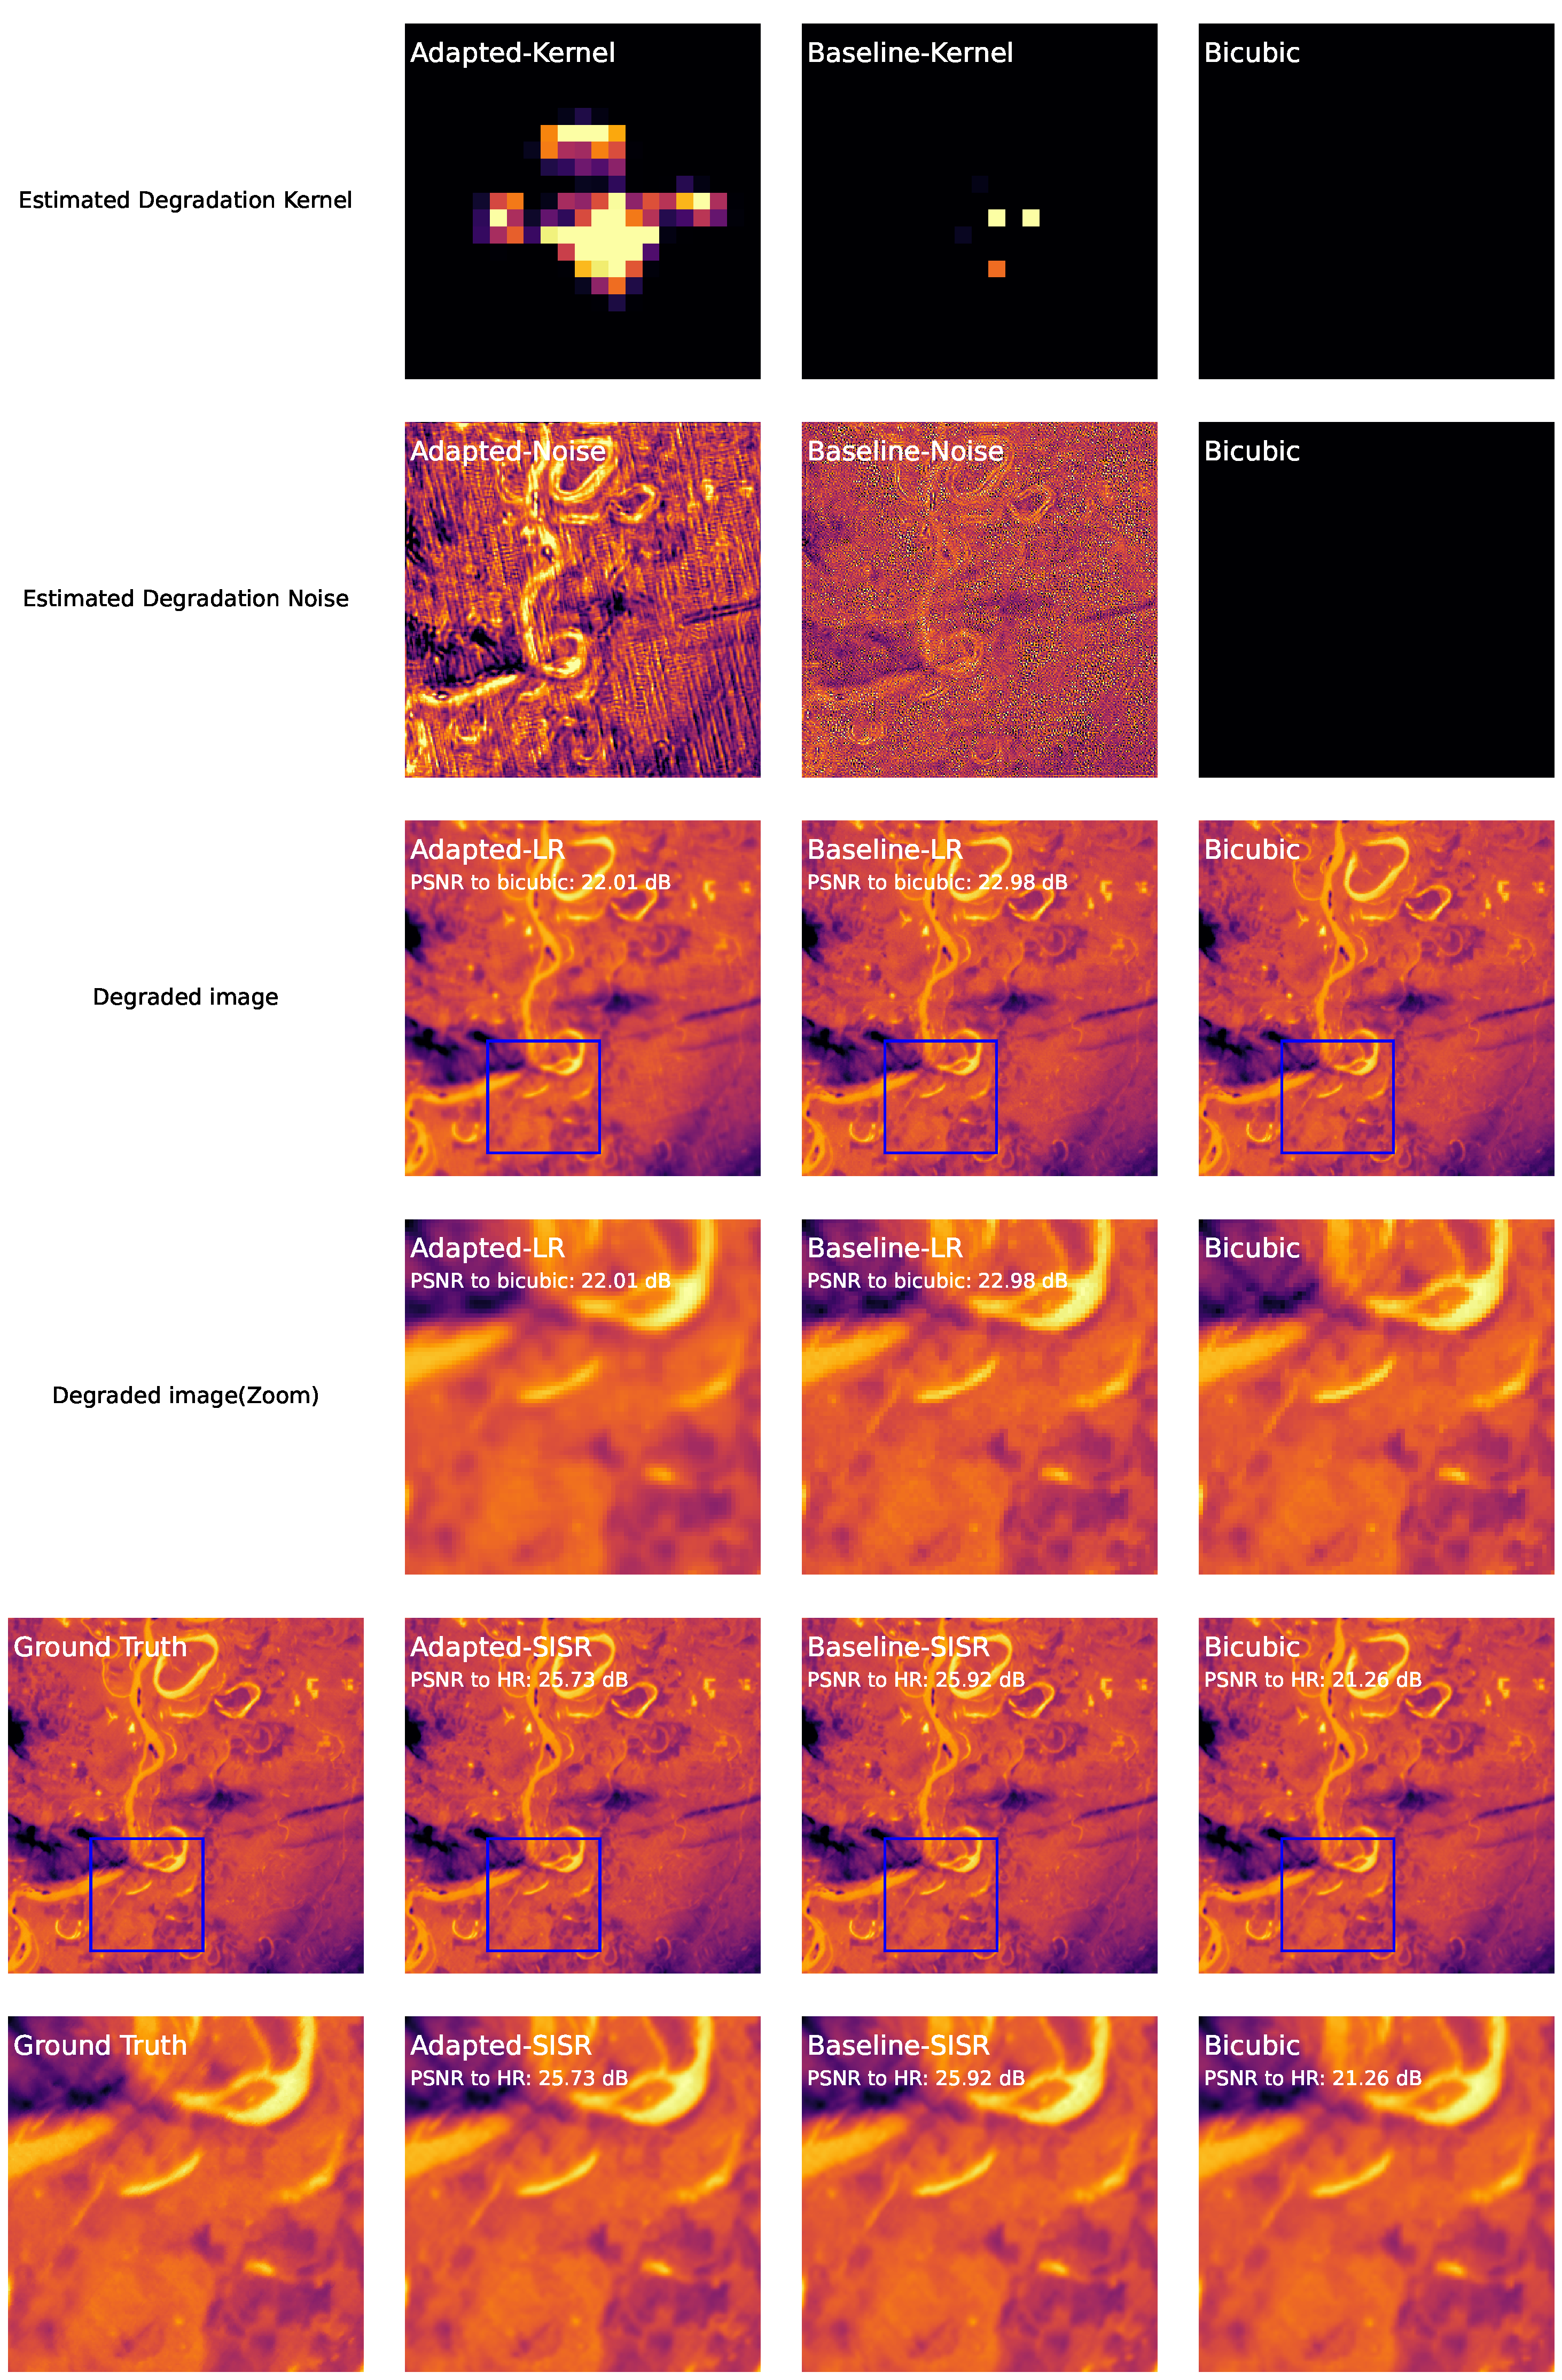
\includegraphics[width=\textwidth]{Includes/5-source-prediction-sample.pdf}
            \caption{Applying different degradation models on an HR sample. 
                     The 2 most upper rows show the estimated degradation kernels and noise of each pipeline, the bicubic downsampling does not estimate a kernel or noise.
                     The degraded LR images from each model and a zoom is displayed on the two subsequent rows. 
                     In this case, the PSNR is calculated against the gaussian blurring + bicubic downsampling LR.
                     The synthetic FOREST-2 (ground truth) and the super resolved images, with a zoom, are displayed in the last 2 rows. 
                     The PSNR for each SR method is calculated against the HR synthetic FOREST-2.
            }
            \label{fig:5-source_domain_sample}
        \end{figure}


        In Figs \ref{fig:5-lr-images-fft.pdf} the frequency domain of the LR images is analyzed.
        By inspection of the FFTs, it is observed that the adapted-LR loses more information than the baseline-LR, as the log magnitude of the FFT get cut more close to the center.
        The baseline-LR FFT is very close to the gaussian blurring + bicubic upsampling FFT, suggesting that the baseline pipeline is able to mimic this known degradation model.

        \begin{figure}[H]
            \centering
            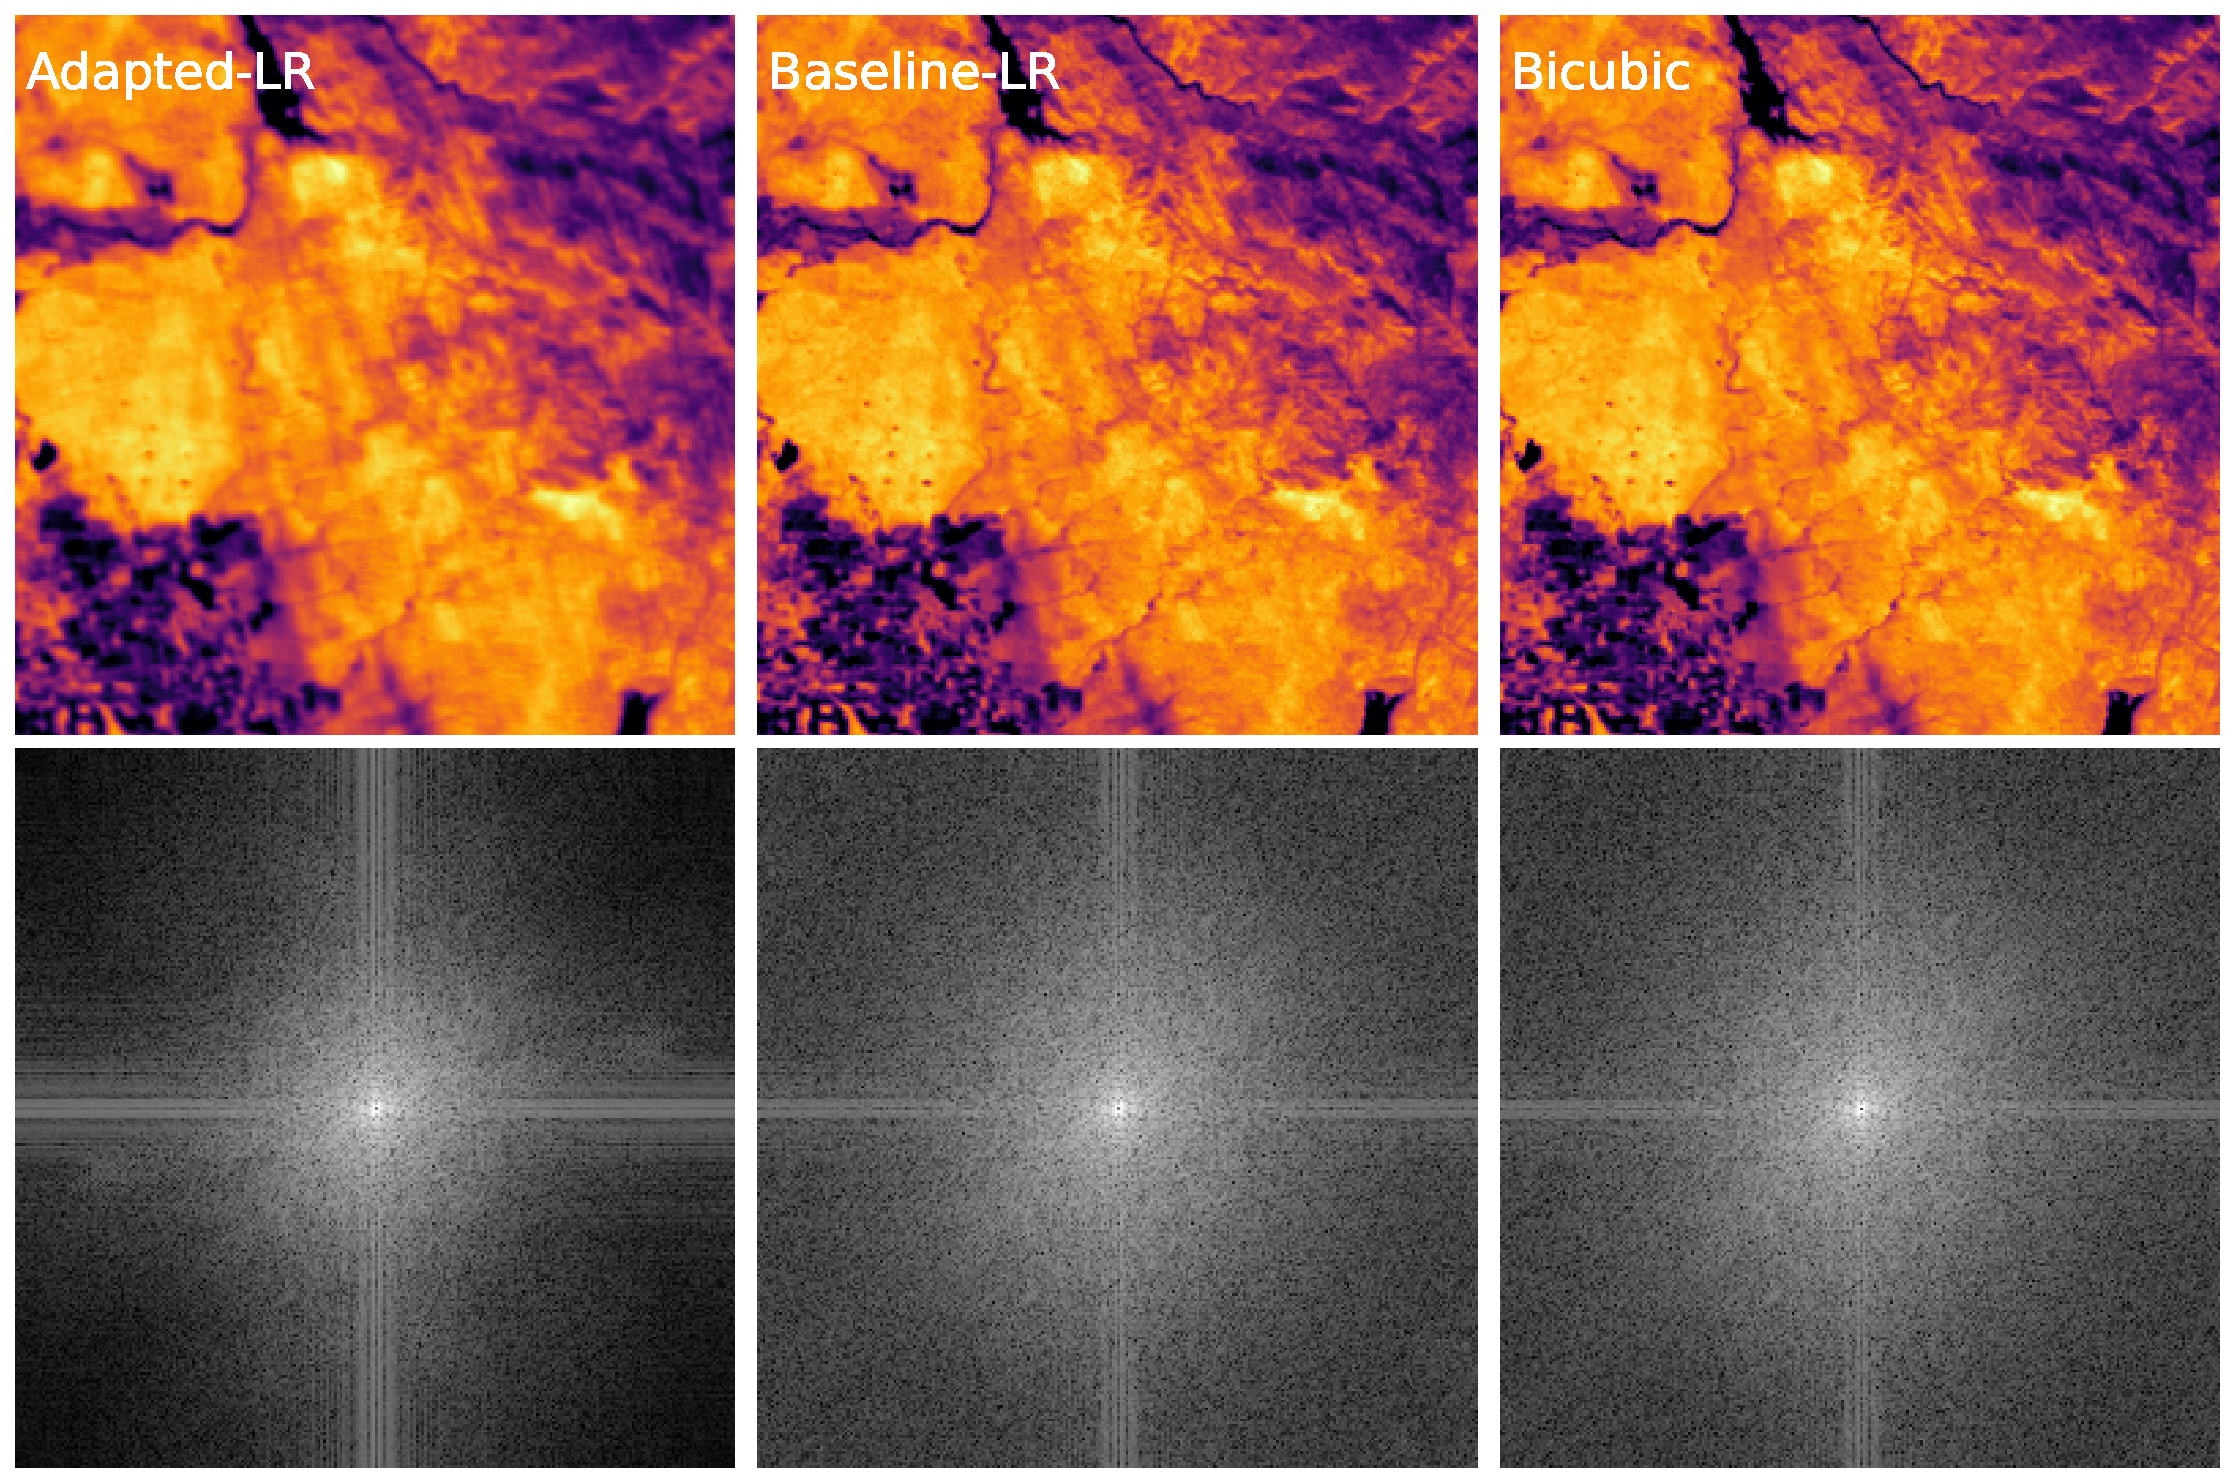
\includegraphics[scale=0.3]{Includes/5-lr-images-fft.pdf}
            \caption{Log mangnitude of the FFT for the LR images obtained by the pipelines and the gaussian blurring + bicubic upsampling.}
            \label{fig:5-lr-images-fft.pdf}
        \end{figure}

        The radial profile of the log magnitude of the FFT for the LR images shown in Fig. \ref{fig:5-lr-images-fft-comparison.pdf} confirmed what was observed previously.
        The adapted-LR image diminishes the high frequency components much more than the baseline-LR image with amplifications of -6dB in frequencies starting at 0.1 cycles per pixel, with a stable effect of -6dB from 0.3 to 0.7 cycles per pixel. 
        It is important to note that 0.1 cycles per pixel at a 210m GSD corresponds to a cycle frequency of 2100m, 0.3 cycles per pixel corresponds to 700m and 0.7 cycles per pixel to 300m.
        This suggests that the degradation model from the real FOREST-2 images is more complex and loses more information than the baseline degradation model.
        An analysis for the whole validation dataset will be further discussed to verify that this behaviour is consistent across different scenes and conditions.


        \begin{figure}[H]
            \centering
            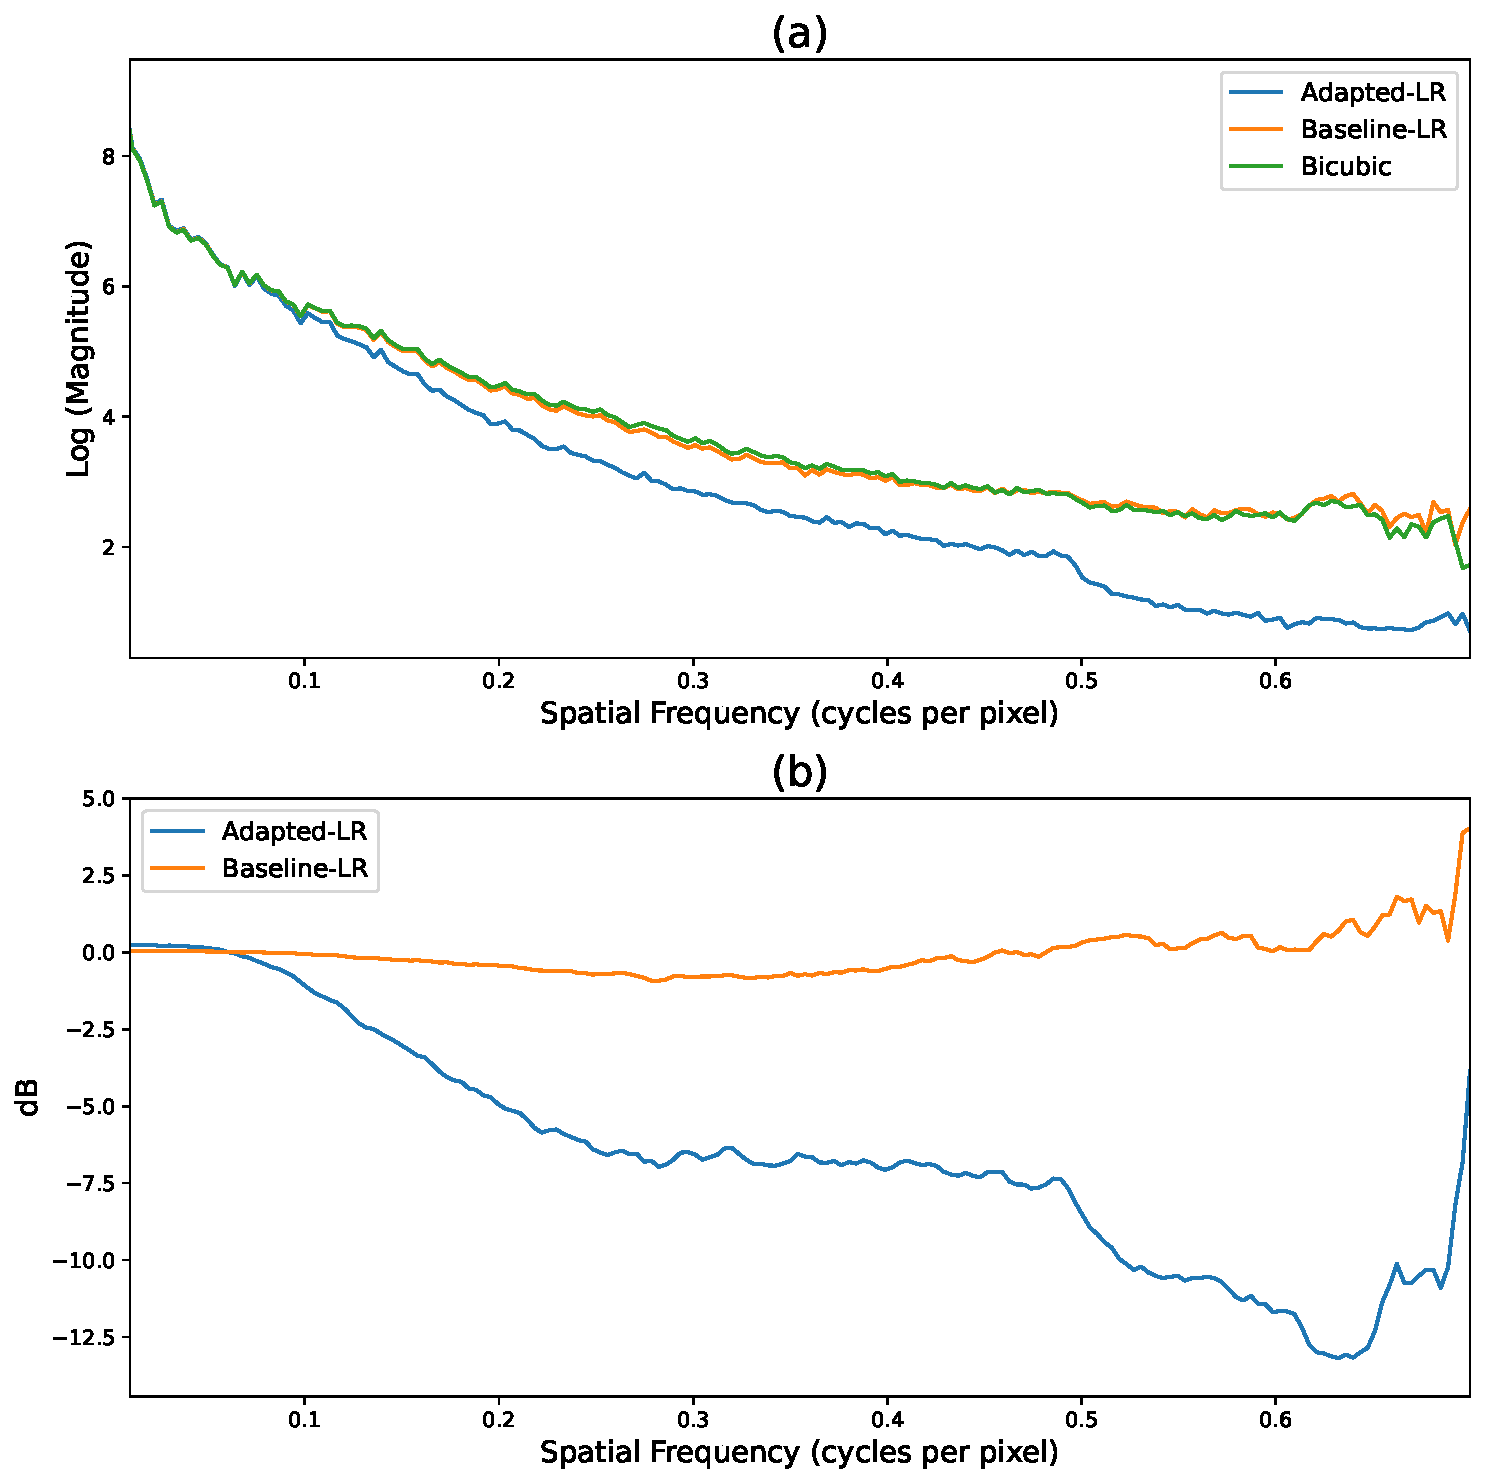
\includegraphics[scale=0.45]{Includes/5-lr-images-fft-comparison.pdf}
            \caption{(a) Radial profile of the log magnitude across spatial frequency of the LR images obtained by the pipelines and the gaussian blurring + bicubic downsampling model.
                     (b) Amplification in dB of each pipeline with respect to the gaussian blurring + bicubic downsampling.}
            \label{fig:5-lr-images-fft-comparison.pdf}
        \end{figure}

        When analyzing the super resolved images versus the ground truth in the frequency domain, a very similar frequency response is observed for the super resolved images of the adapted and the baseline pipelines.
        Moreover, the SR images are able to stay above -3dB, a common threshsold used in the literature, up until 0.3 cycles per pixel, which correspond to 300$\frac{1}{m}$ when each pixel equals 70m.
        This suggests that the SR model in the adapted pipeline is able to recover the lost information at those frequencies due its more complex degradation model.
        Starting at 0.3 cycles per pixel, a decrease in amplification is observed for both pipelines, but more steeply for the adapted pipeline.
        This may be related to the fact that the adapted degradation model diminishes cycles at higher frequencies even more than the baseline degradation model. 
        A limit for the SR algorithm is also noted, even using an optimistic degradation model such as the baseline, the SR model is not able to recover higher frequencies with respect to the original, HR image.
        Even if it is slightly better than bicubic upsampling, the diminishing of the higher frequency components is dramatic.

        \begin{figure}[H]
            \centering
            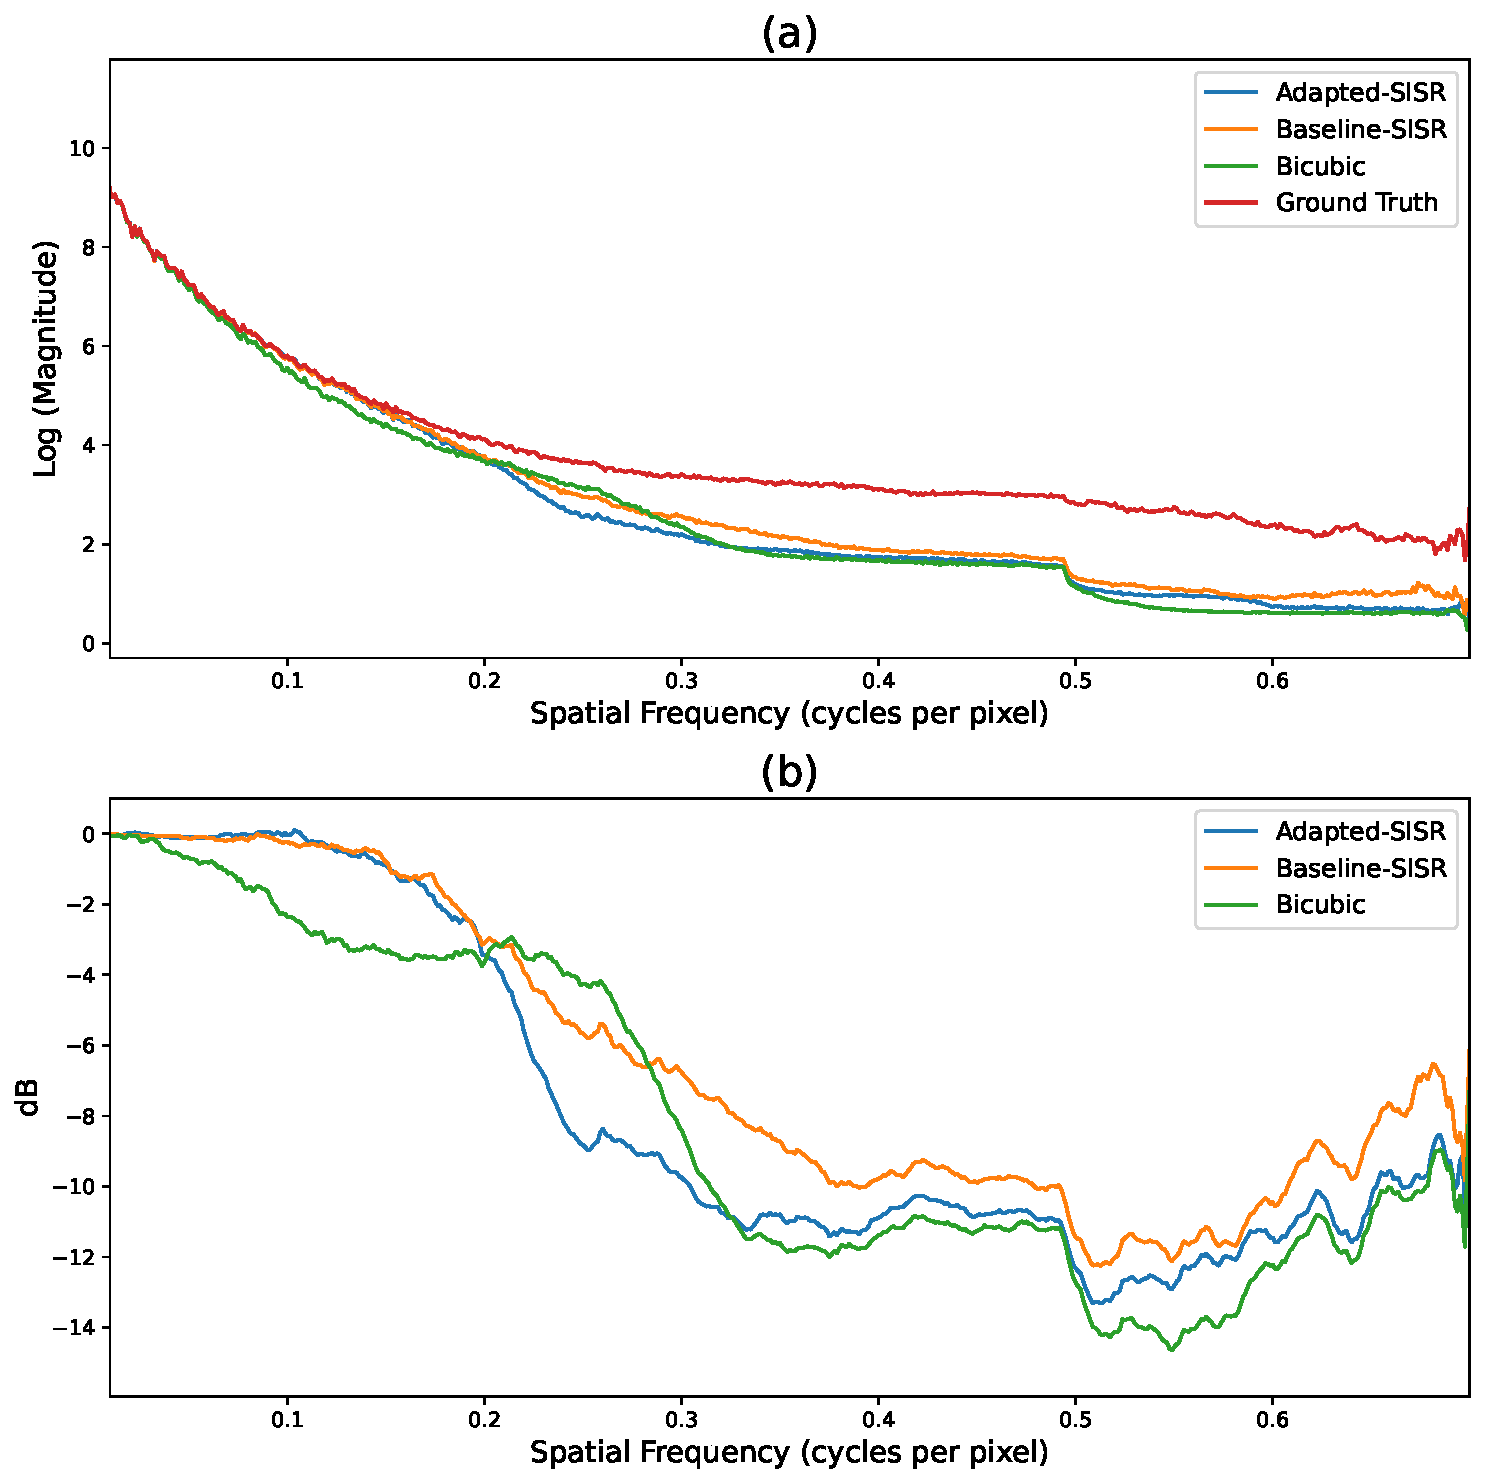
\includegraphics[scale=0.5]{Includes/5-source-sr-fft-comparison.pdf}
            \caption{Frequency domain analysis of the SR images and the ground truth displayed in \ref{fig:5-source_domain_sample}.
                     In (a), the log of the magnitude of the FFT for the SR images and the ground truth is shown,
                     while in (b), the amplification of each SR image with respect to the ground truth is shown.}
            \label{fig:5-source-sr-fft-comparison}
        \end{figure}


        \subsubsection{LR comparison}

        A quantitative analysis of the LR images obtained by the generator of each pipeline is performed. 
        Fig. \ref{fig:5-source-domain-lr-performance-scatterplot} shows 3 supervised performance metrics obtained by comparing the LR images obtained by the pipelines with the gaussian blurring + bicubic downsampling degradation.
        In this case, a consistent higher PSNR and SSIM means that the baseline-LR image is closer to the gaussian blurring + bicubic downsampling LR image than the one generated by the adapted pipeline. 
        A lower LPIPS means that even using perceptual metrics, the baseline-LR image is also closer.
        This is consistent with the results shown in Fig. \ref{fig:5-source_domain_sample}, where the adapted LR image is more blurry and noisy, suggesting that the unknown degradation is worse than the baseline degradation model.
        
        \begin{figure}[H]
            \centering
            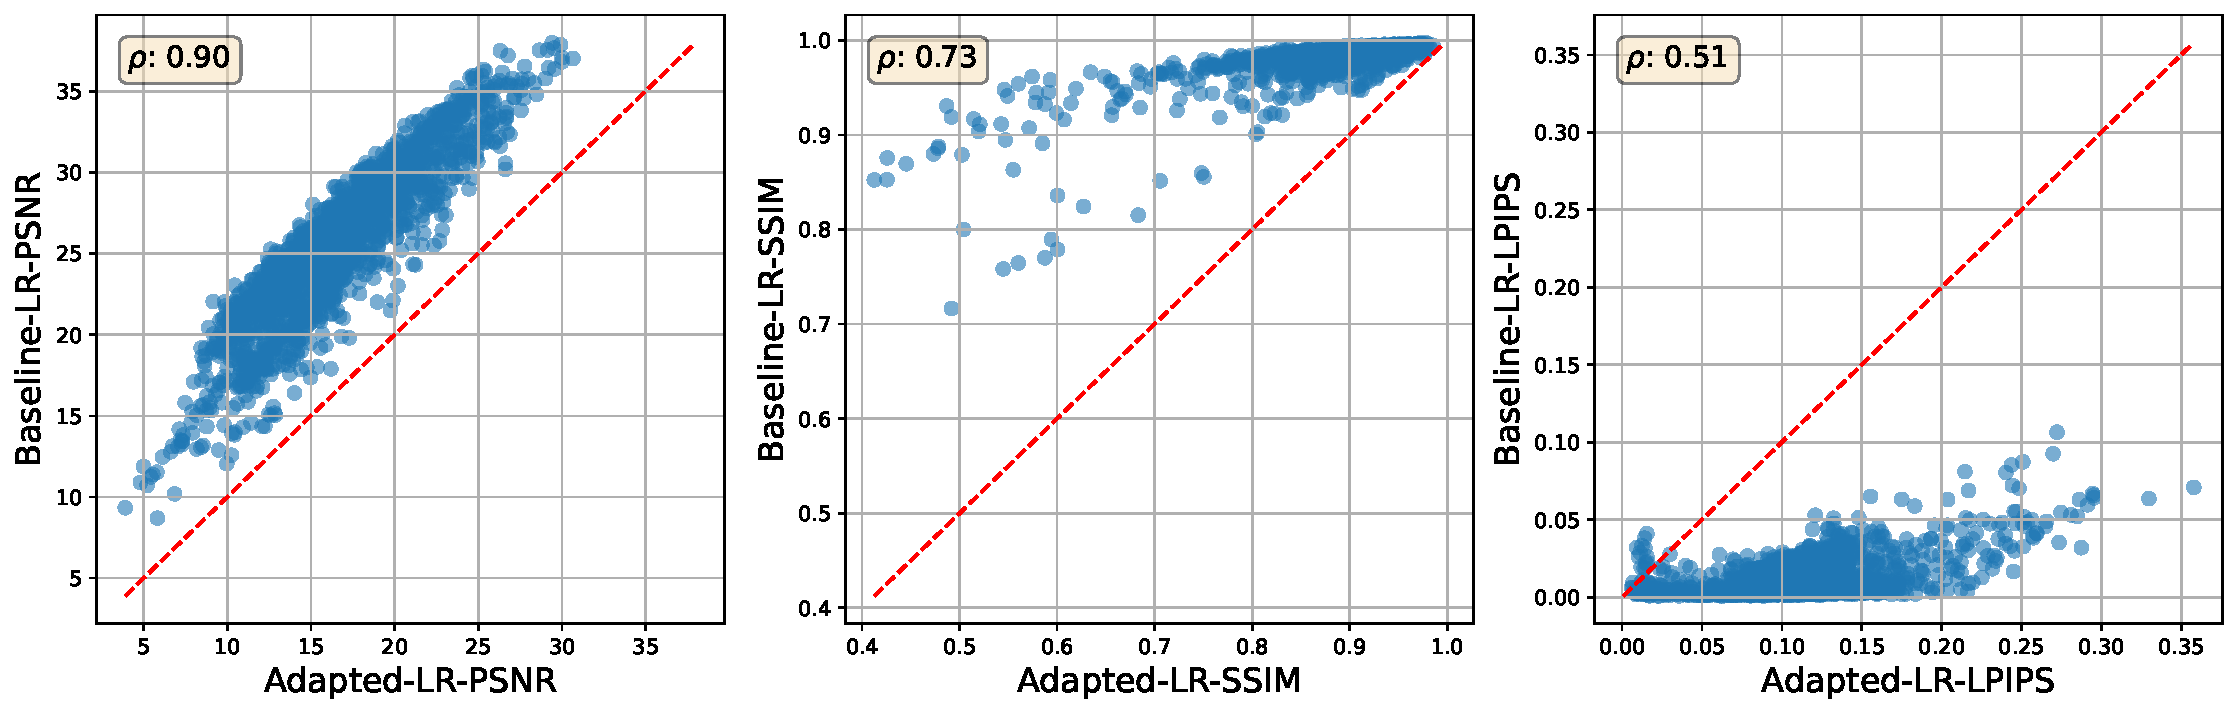
\includegraphics[width=\textwidth]{Includes/5-source-domain-lr-performance-scatterplot.pdf}
            \caption{Performance metrics between the LR images obtained by the pipelines vs the gaussian blurring + bicubic downsampling degradation.}
            \label{fig:5-source-domain-lr-performance-scatterplot}
        \end{figure}




        An alternative way to evaluate the differences in the degradations is by analyzing the frequency domain of the LR images.
        An analysis of the whole validation dataset is performed by calculating the FFT of each LR image and comparing them with the gaussian blurring + bicubic downsmapling degradation model.
        The results are displayed shown in Fig. \ref{fig:5-lr-images-fft-comparison}. 
        In (a) the log magnitude of the FFT across different spatial frequency values for the degraded images is shown. 
        The spatial frequency is obtained from the radial distance to the center of the FFT, as shown in \ref{subsubsec:frequency_domain_analysis}.
        In (b), the amplification of each generated LR image with respect to a simple gaussian blurring + downscaling is shown. 
        The results for the whole dataset show that the LR images generated by the adapted pipeline yield a reduction in the higher frequency components consistently across all samples, with a ± 1 standard deviation interval between -4 and -6 dB from between 0.3 and 0.7 cycles per 210m pixel.
        This translates in blurrier images, and a more difficult starting point for a SR model to work with.

        \begin{figure}[H]
            \centering
            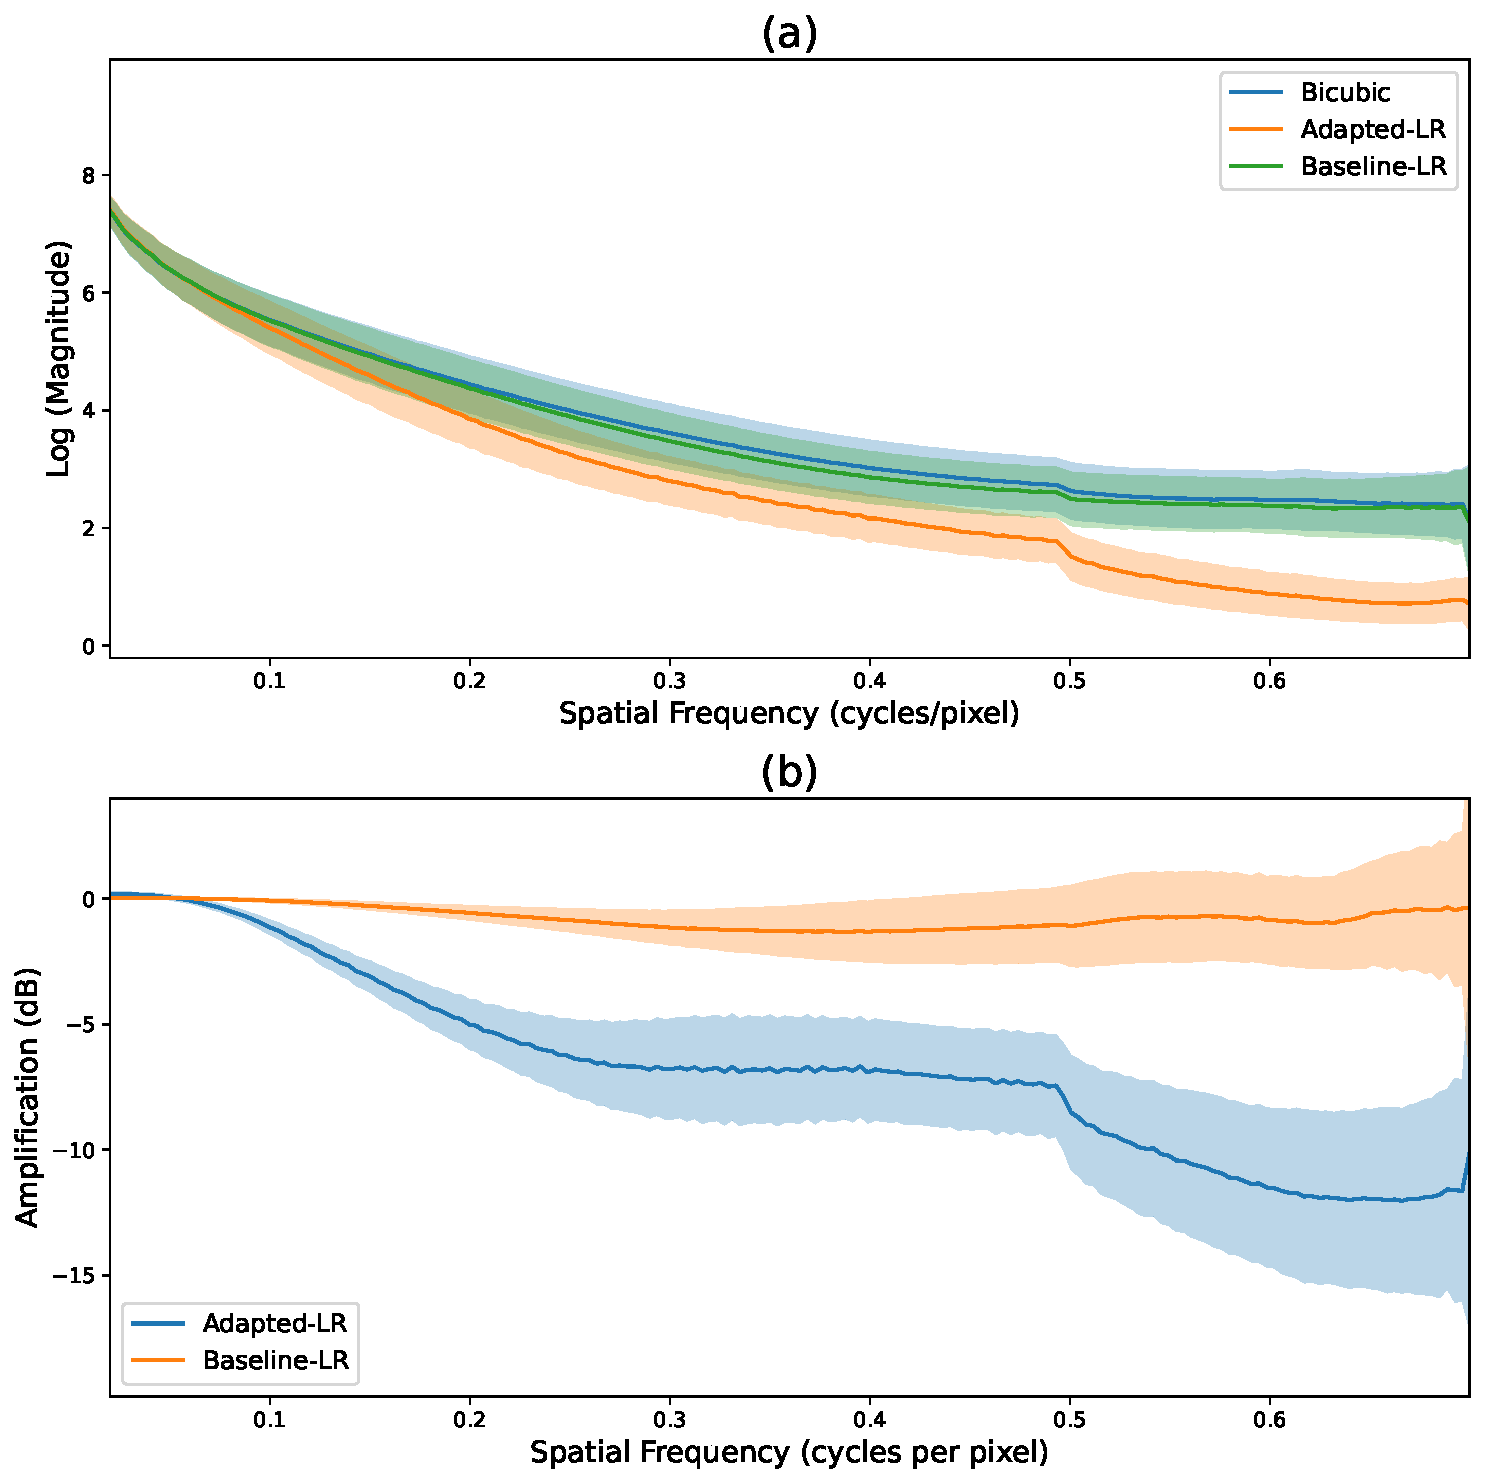
\includegraphics[scale=0.5]{Includes/5-source-lr-amplification-statistics.pdf}
            \caption{Frequency domain analysis of the LR images obtained by applying different degradation models on the HR sample displayed in Fig. \ref{fig:5-source_domain_sample}.
                     In (a), the log of the magnitude of the FFT for the LR images is shown,
                     while in (b), the amplification with respect to a  simple gaussian blurring + downscaling is shown.
                     The painted area represents the ±1 standard deviation of the radial profiles and the amplification. }
            \label{fig:5-lr-images-fft-comparison}
        \end{figure}




        \subsubsection{Effects of the degradation model in SR}

        Another subject of interest is how the degradation model affects the performance of the super resolution process.
        Fig. \ref{fig:5-source-domain-comparison} shows the performance obtained by super resolving the output of each pipeline generator for the whole validation dataset.
        In the upper row (a), the corresponding SR model of each pipeline is used to obtain the super resolved images. 
        The performance, both in PSNR and SSIM, are very similar for both pipelines. The LPIPS shows a consistent behavior too.
        In the lower row (b), the SR model is discarded and a simple bicubic upsampling is used to super resolve the degraded images of each pipeline. 
        In this case, using the baseline LR version as input consistently yields better results than the adapted LR version, in all metrics.
        This suggests that the learned degradation model from FOREST-2 images loses more information than the baseline, resulting in a lower effective ground sampling distance than what was is specified in FOREST-2 fact sheet.
        Consistent with what was found in the frequency domain analysis observed in Fig. \ref{fig:5-source-sr-fft-comparison}, the SR model is able to recover most of the information, as the performance after using the SR models is very similar. 
        
        \begin{figure}[H]
            \centering
            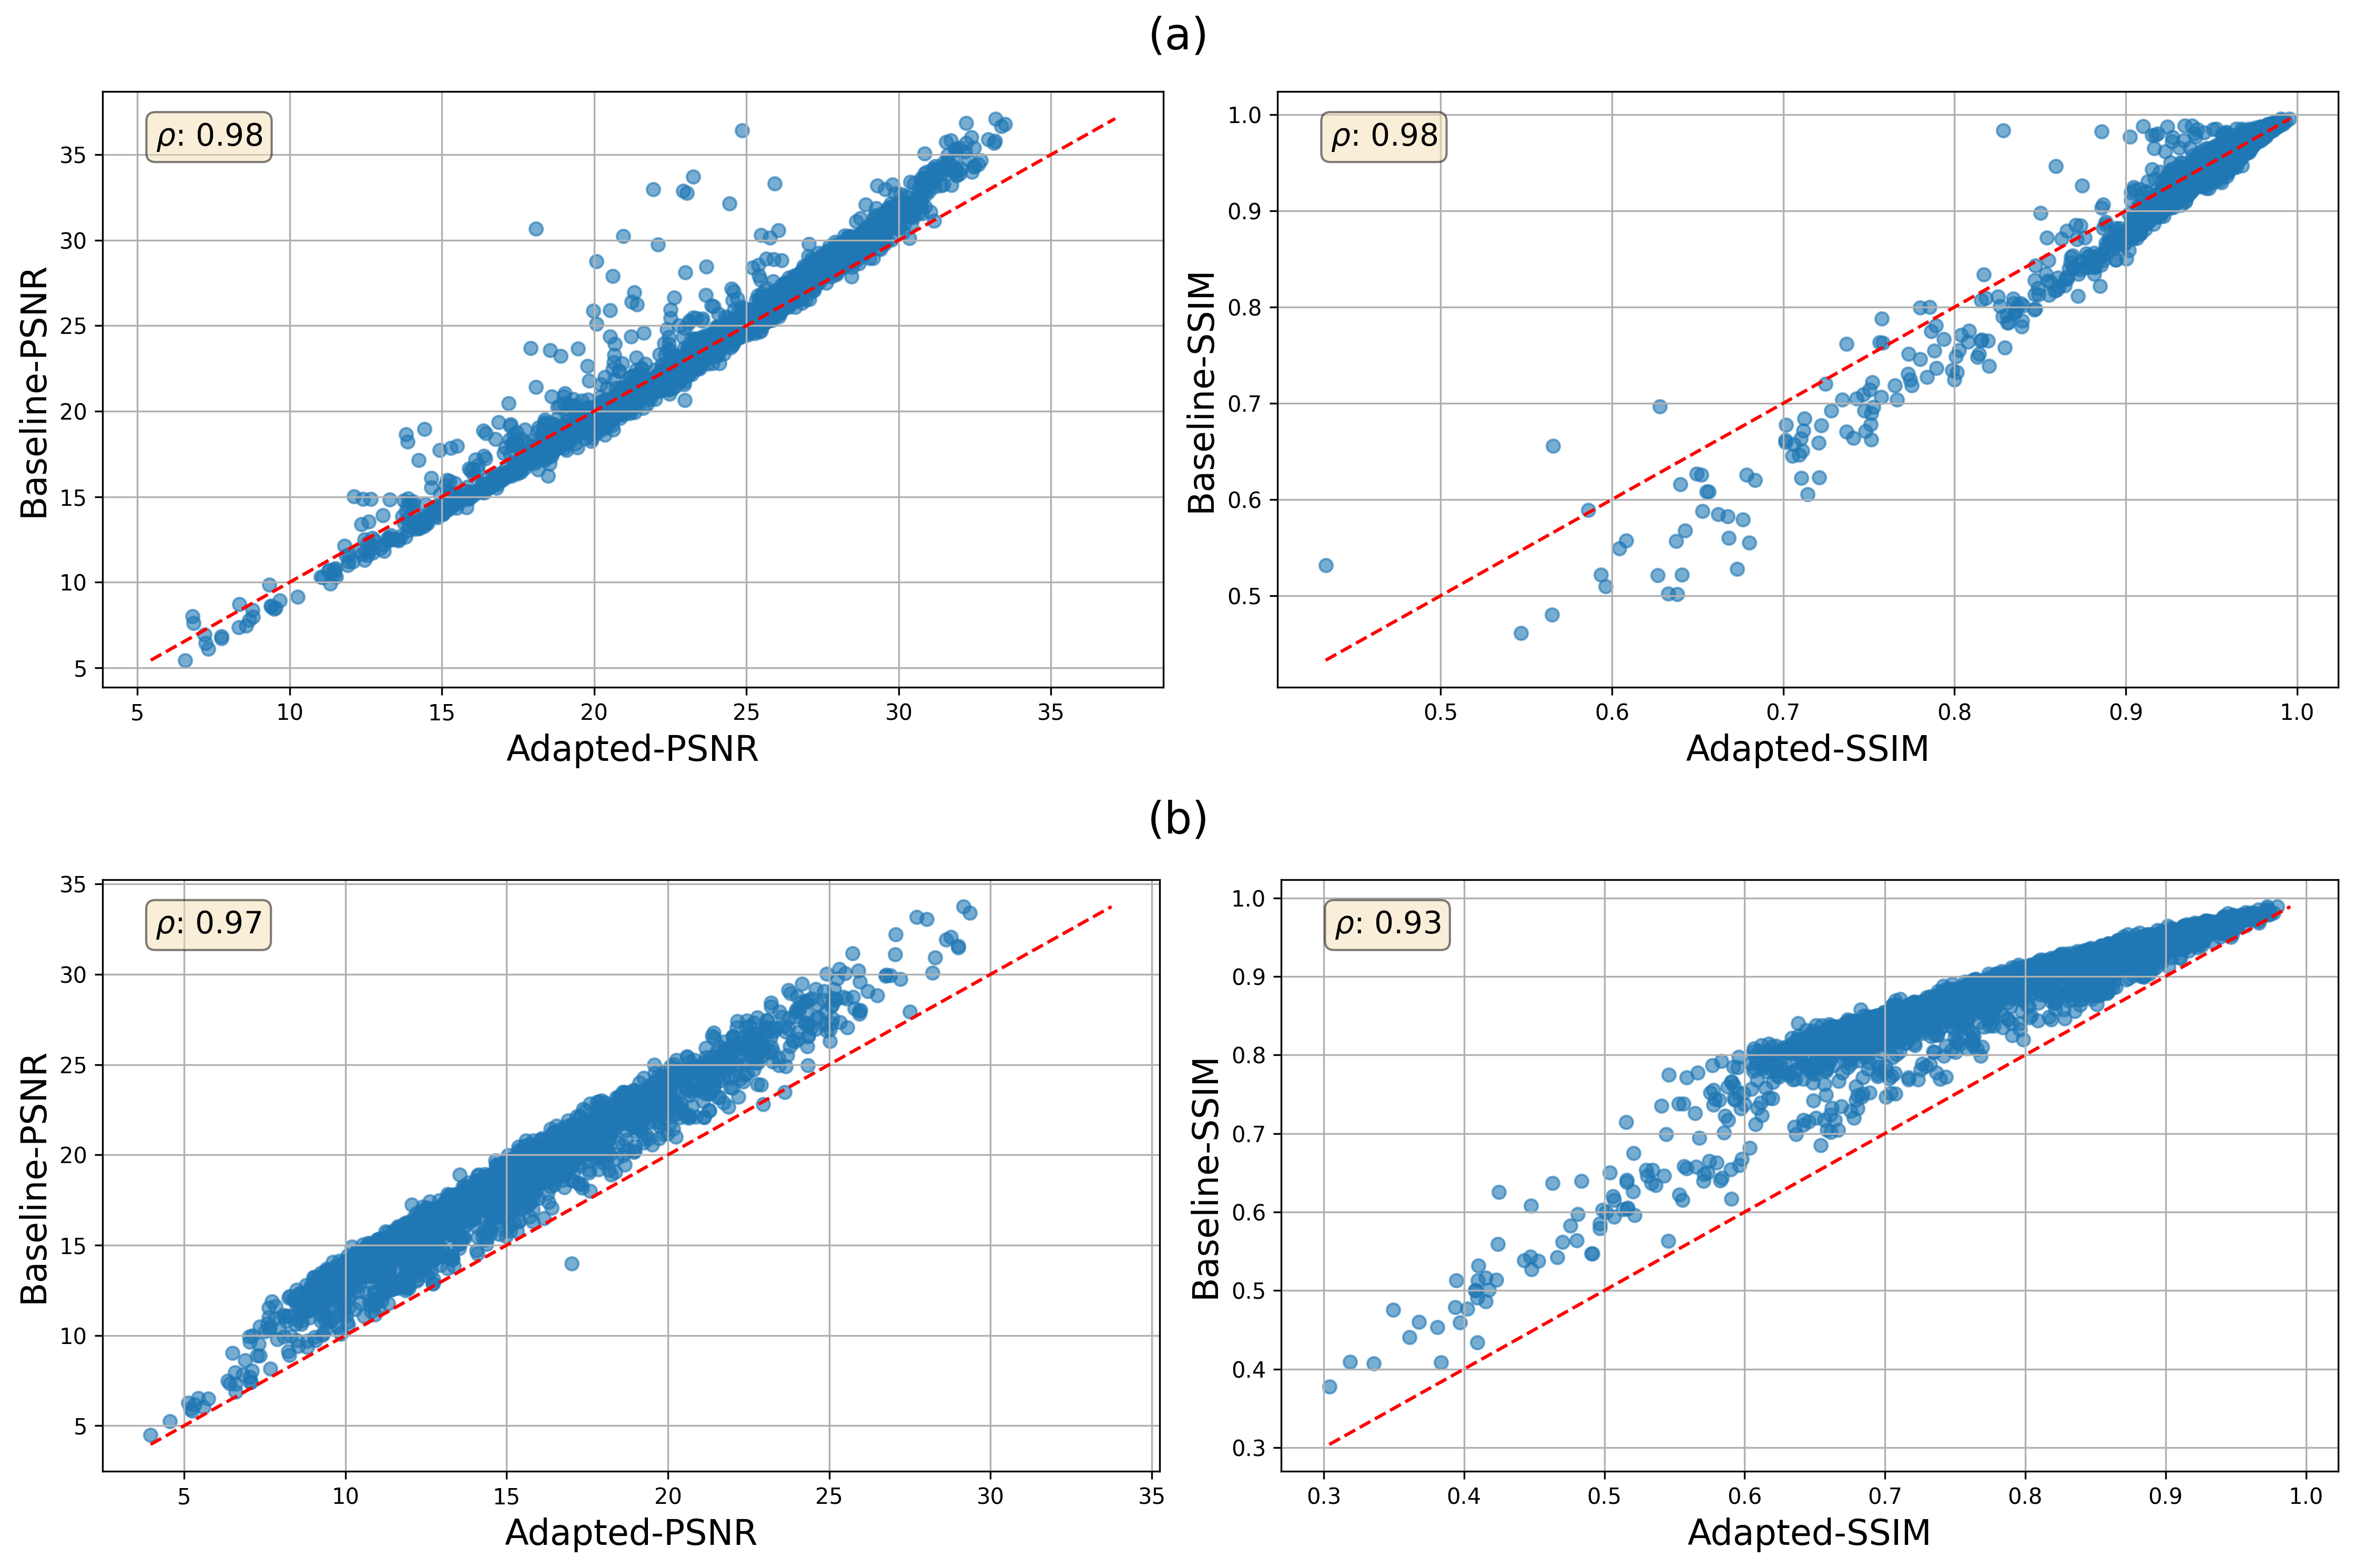
\includegraphics[width=\textwidth]{Includes/5-source-domain-comparison.png}
            \caption{Performance obtained by super resolving the degraded images coming out of the generator. 
                     In (a), the corresponding SR model of each pipeline is used. 
                     In (b), a simple bicubic upsampling is used to super resolve the degraded images. }
            \label{fig:5-source-domain-comparison}
        \end{figure}

        Fig \ref{fig:5-source-domain-comparison} proves the relevance of the domain gap in super resolution, the SR model is able to estimate the inverse of the degradation function in most cases, if given the correct data.
        The problem relies on that in most experiments, the wrong degradation is shown to the model, forcing it to learn the inverse of an incorrect function.  
        This plays an essential role when deploying super resolution model in real production environments, where the degradation model may not be known. 

    \subsection{Target domain}

        This subsection will show the results from the experiments performed on the target domain, which is the equivalent of the red arrows flow described in fig. \ref{fig:3-GAN-degradation-model}.
        In this case, the GAN trained for the degradation model is discarded and only the super resolution model is used.
        The input images are real FOREST-2 images, and the output images are super resolved versions of them. 
        Due to the unpaired nature of the dataset, the performance of the SR model can not be evaluated using metrics like PSNR and SSIM. 
        Other alternatives will be presented, and a qualitative analysis will be performed. 
        Additionally, a quantitative analysis will be discussed using a very small sample of paired data obtained by synchronizing the overpass of FOREST-2 with the route of ECOSTRESS.


        In Fig. \ref{fig:5-target_prediction_sample}, the super resolution models were used with a 264x264 pixels crop of a real FOREST-2 image as an input.
        The results show that the baseline model, trained with $\mathcal{D}_{\text{SF}-\text{SF}}$, has very similar results to bicubic upsampling.
        On the other side, the adapted model, trained using real FOREST images as the target domain ($\mathcal{D}_{\text{SF}-\text{RF}}$), is able to recover more details, producing sharper images.
        In the frequency domain, the effects of super resolution are clear, frequency components of interest are amplified compared to bicubic upsampling, without over-amplifying higher frequencies usually related to noise.
        
        


        \begin{figure}[H]
            \centering
            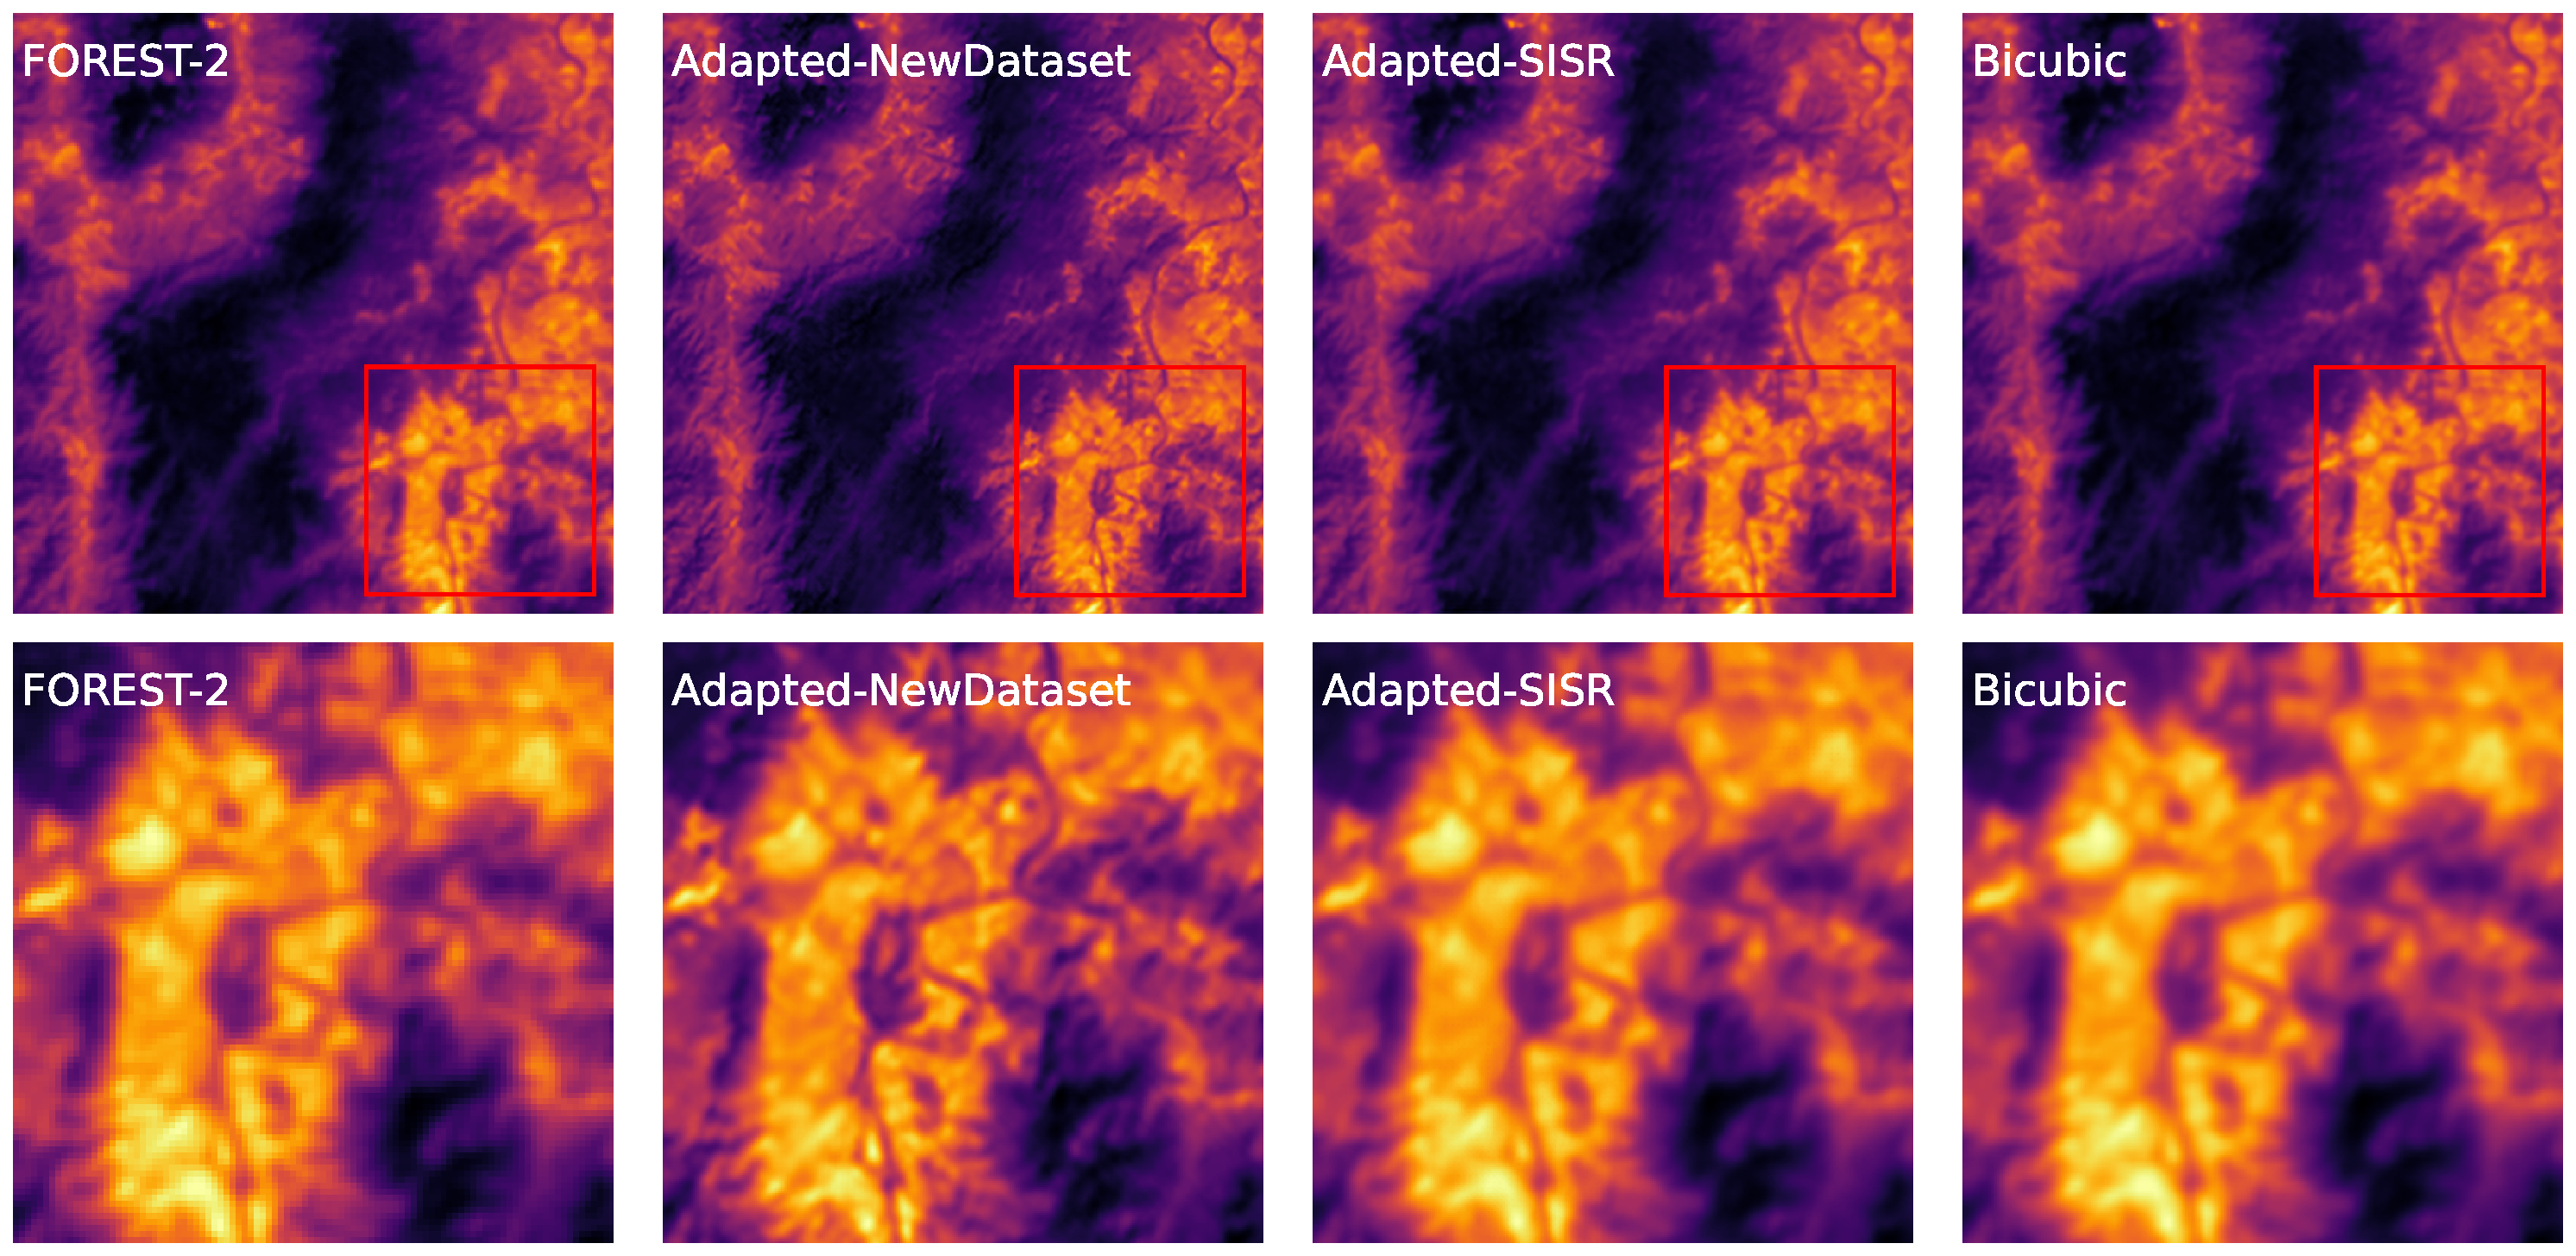
\includegraphics[scale=0.28]{Includes/5-target_prediction_sample.pdf}
            \caption{Super Resolved Forest-2 Scene using different SR models.
                     In the upper row, the image is displayed. A detailed zoom is displayed below. The bottom row shows the log magnitude of the FFT for the images.
                     The original image is displayed in the left, while the super resolved images are displayed afterwards.
                    }
            \label{fig:5-target_prediction_sample}
        \end{figure}

        % The results of Fig. \ref{fig:5-target_prediction_sample} with the theory and the results obtained in the source domain.
        % The super resolutions task is to estimate the inverse function of the degradation process. 
        % When the model is trained using an optimistic degradation process, the model is snot able to recover details from images generated by a more complex degradation process, like the real FOREST-2 images.
        % The lack of details in the baseline-SISR images is not because the model is not able to recover them, but because a more optimistic degradation model was used in training. 
        % This is an important result to drive the attention to the importance of the degradation model used in training, instead of focusing on more complex super resolution architectures.

        Fig. \ref{fig:5-target-amplification-statistics} shows a more detailed analysis of the frequency domain of the SR images obtained by applying different SR models to the whole FOREST-2 validation dataset.
        In (a),the log magnitude of the FFT for the SR images is displayed, adding a shade that represent the interval of ±1 standard deviations. 
        Up until 0.3 cycles per pixel, the adapted model has a higher log magnitude than the baseline SR model or bicubic upsampling, also staying slightly higher in high frequency components.
        As higher frequencies are related to noise and artifacts, this suggests that the adapted model is able to recover more details than the baseline model, while minimizing undesired components.
        The amplification plot of the SR models against bicubic upsampling shows the same behaviour in a more clear way. Between 0.1 and 0.25 cycles per pixel, the amplification peaks  between 6 and 8 dB on average with respect to bicubic, while the baseline model is between 0 and 2 dB.
        Such amplification, at a pixel size of 70m, corresponds to cycle frequencies between  300 $\frac{1}{m}$ and 700 $\frac{1}{m}$, which is consistent with the loss of components observed in \ref{fig:5-lr-images-fft-comparison}.
        The variability of the amplification allows to conclude that this amplification is consistently higher than the baseline-SISR for all the validation dataset.
        On the other side, while the amplification is very similar in frequencies related to noise, the adapted model seems to step up a little bit compared to the baseline.  
        This suggests that the adapted model is able to recover details from real FOREST-2 images, amplifying frequencies of interest, at the cost of a small increase in the overall noise of the image.

        \begin{figure}[H]
            \centering
            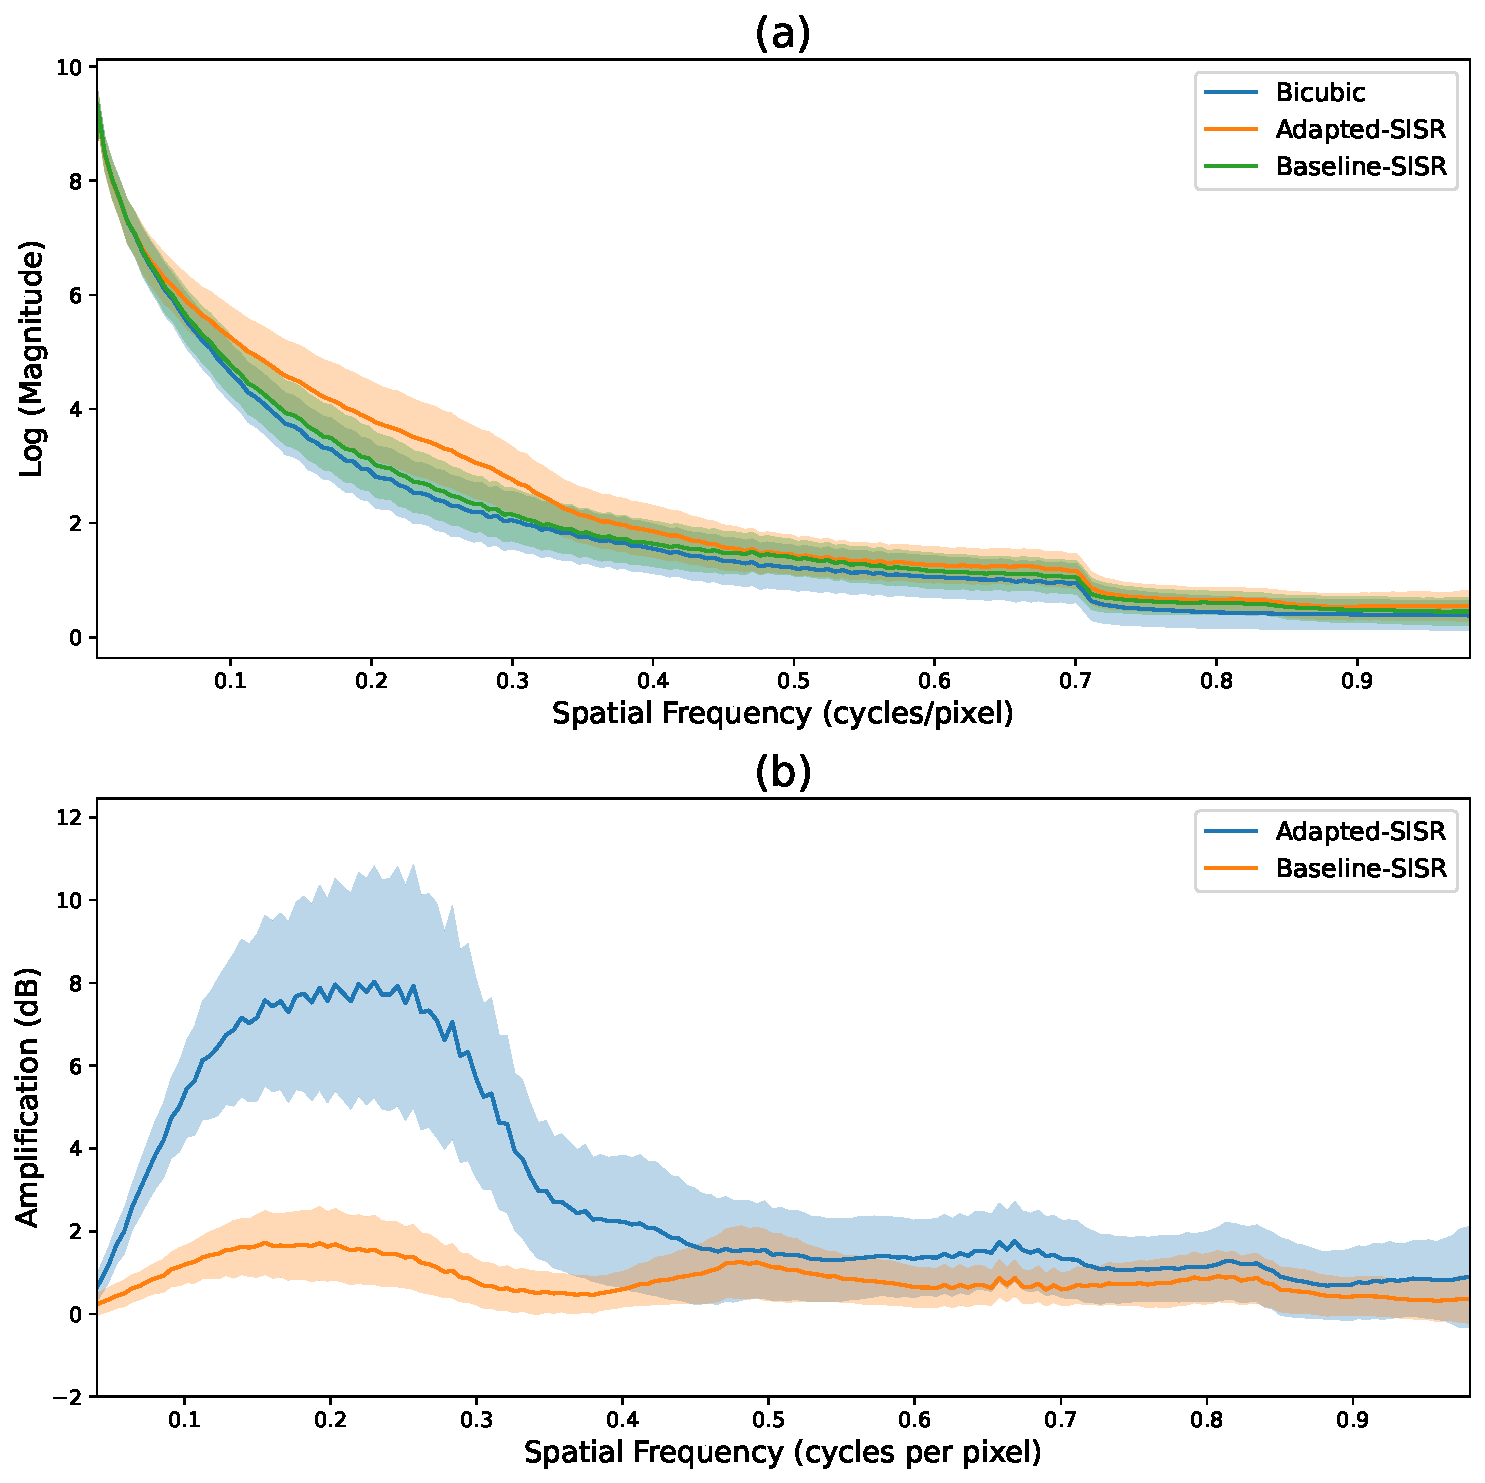
\includegraphics[scale=0.5]{Includes/5-target-amplification-statistics.pdf}
            \caption{Frequency domain analysis of the SR images obtained by applying different SR models to the real FOREST-2 validation dataset.
            In (a), the log of the magnitude of the FFT for the SR images is shown,
            while in (b), the amplification with respect to a  simple bicubic upsampling is displayed.}
            \label{fig:5-target-amplification-statistics}
        \end{figure}


        In Fig. \ref{fig:6-target-gradient-analysis-image}, an example of the gradient analysis of the SR images is shown. 
        Compared to the baseline SISR model, the adapted model shows higher gradient magnitudes, suggesting that the adapted model is able to recover more details than the baseline model. 
        However, in the more dark sections of the gradient magnitude, some small background noise can be percieved, consistent with the results of the frequency domain analysis.

        \begin{figure}[H]
            \centering
            \includegraphics[scale=0.28]{Includes/6-target-gradient-analysis-image.pdf}
            \caption{Gradient analysis of the super resolved images using different SR models for scenes coming from the real FOREST-2 validation dataset.
                     In the upper row, the image is displayed. The gradients in the x and y direction ($G_x$ and $G_y$ respectiely) are displayed below.
                     the gradient magnitude $|G|$ is displayed in the bottom row.}
            \label{fig:6-target-gradient-analysis-image}
        \end{figure}

        Fig \ref{fig:5-gradient-histogram-validation-dataset} shows the distribution function of the gradient magnitudes of the whole validation dataset, estimated through a histogram.
        Both the adapted and the baseline model show a decrease in the number of pixels with low gradient magnitudes, suggesting that both models are able to recover more details than bicubic upsampling.
        However, the adapted model shows a higher number of pixels with high gradient magnitudes, implying that the adapted model is able to produce sharper edges than the baseline model.
        This is consistent with the observed results and the frequency domain analysis. 
        However, it is important to note that the gradient magnitude is not a good measure of the performance of the SR model, as it does not take into account the noise and artifacts that may be present in the image.
        It represents only a complementary way to understand the effects of the SR model.


        \begin{figure}[H]
            \centering
            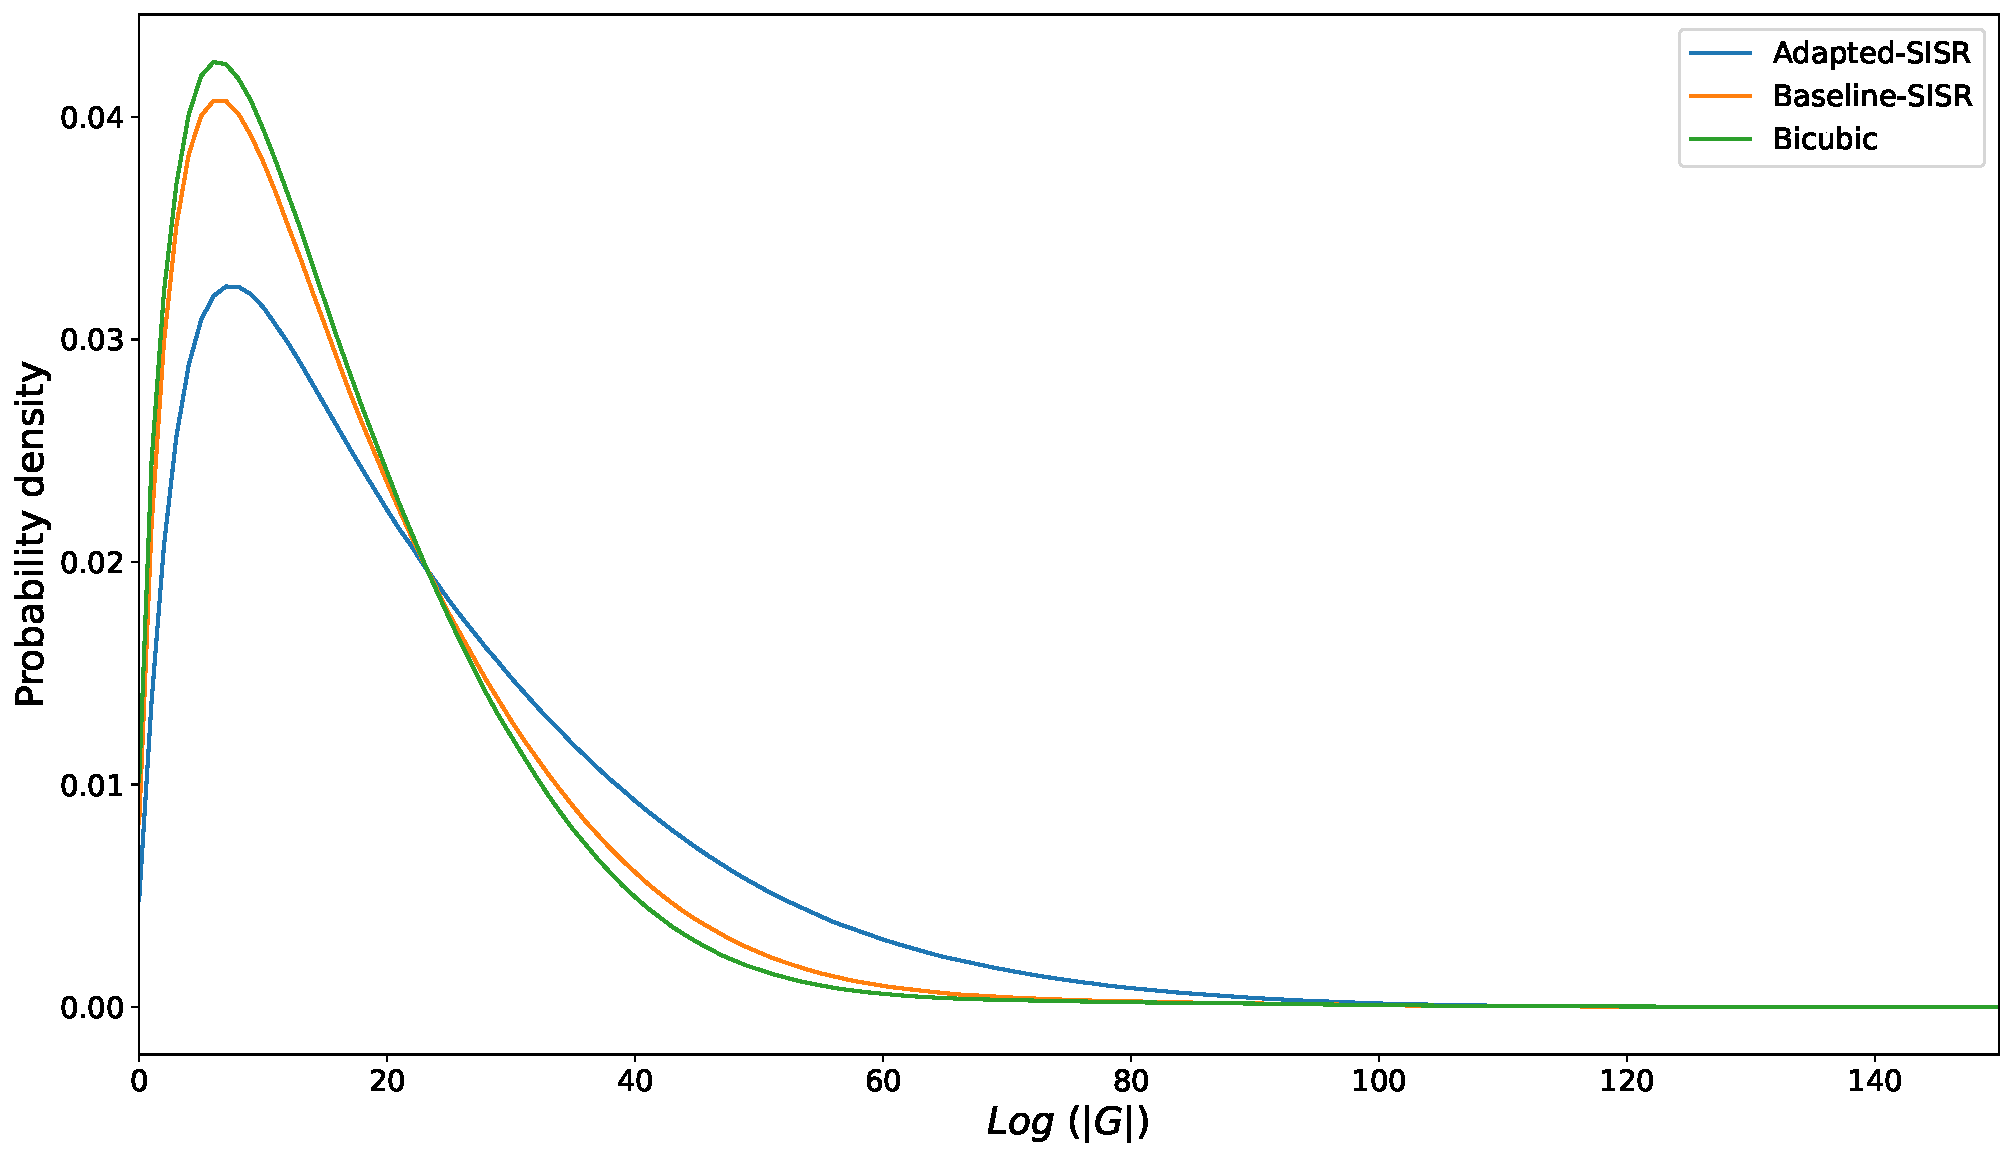
\includegraphics[scale=0.4]{Includes/5-gradient-histogram-validation-dataset.pdf}
            \caption{Histogram of the gradient magnitude $|G|$ for the whole validation real FOREST-2 dataset.}
            \label{fig:5-gradient-histogram-validation-dataset}
        \end{figure}

    \subsection{The domain gap goes both ways}

         % Another example would be images taken from FOREST-2 in several years may not have the same distribution as current images, as the instruments may have degraded over time.

        To simulate this situation, the model trained using real FOREST-2 images was employed to super-resolve synthetic FOREST images degraded using the baseline degradation model. The results, shown in Figs. \ref{fig:5-target-prediction-with-domain-gap} and \ref{fig:5-target-prediction-with-domain-gap-fft}, indicate the performance of the adapted model is catastrophic, producing several artifacts and yielding a PSNR difference of approximately 10dB, which represents a tenfold difference in terms of Mean Squared Error (MSE). This highlights the critical need for adaptable SR models that can effectively handle diverse and evolving real-world scenarios.


        The combination of the probabilistic degradation model and the SR model were proven helpful to bridge the domain gap and inprove the resolution of real FOREST-2 images.
        However, it is important to understand what happens when the target domain used in training does not match the conditions that will occur in the real world.
        While the common scenario is that the real degradation model is more complex than the one assumed in the experiments, the opposite can also occur.
        Assuming a more complex degradation model in the dataset could lead to generated LR images with more attenuation in the frequency domain, resulint in an SR model that "over-amplifies", producing noisy images with undesired artifacts.
        In this work, HR-LR pairs generated using a baseline degradation model exemplify an overly optimistic degradation scenario.
        When using the adapted SR model on these generated LR images, this second scenario can be analyzed.
        As in this experiment, the ground truth is known, the performance of the SR model can be evaluated using metrics like PSNR and SSIM.
        
        The results are shown in Figs. \ref{fig:5-target-prediction-with-domain-gap} and \ref{fig:5-target-prediction-with-domain-gap-fft}.
        The performance of the adapted model on images with an optimistic degradation model is catastrophic, producing several artifacts and yielding a PSNR difference of approximately 10dB, which represent a 10x difference in terms of MSE.

        \begin{figure}[H]
            \centering
            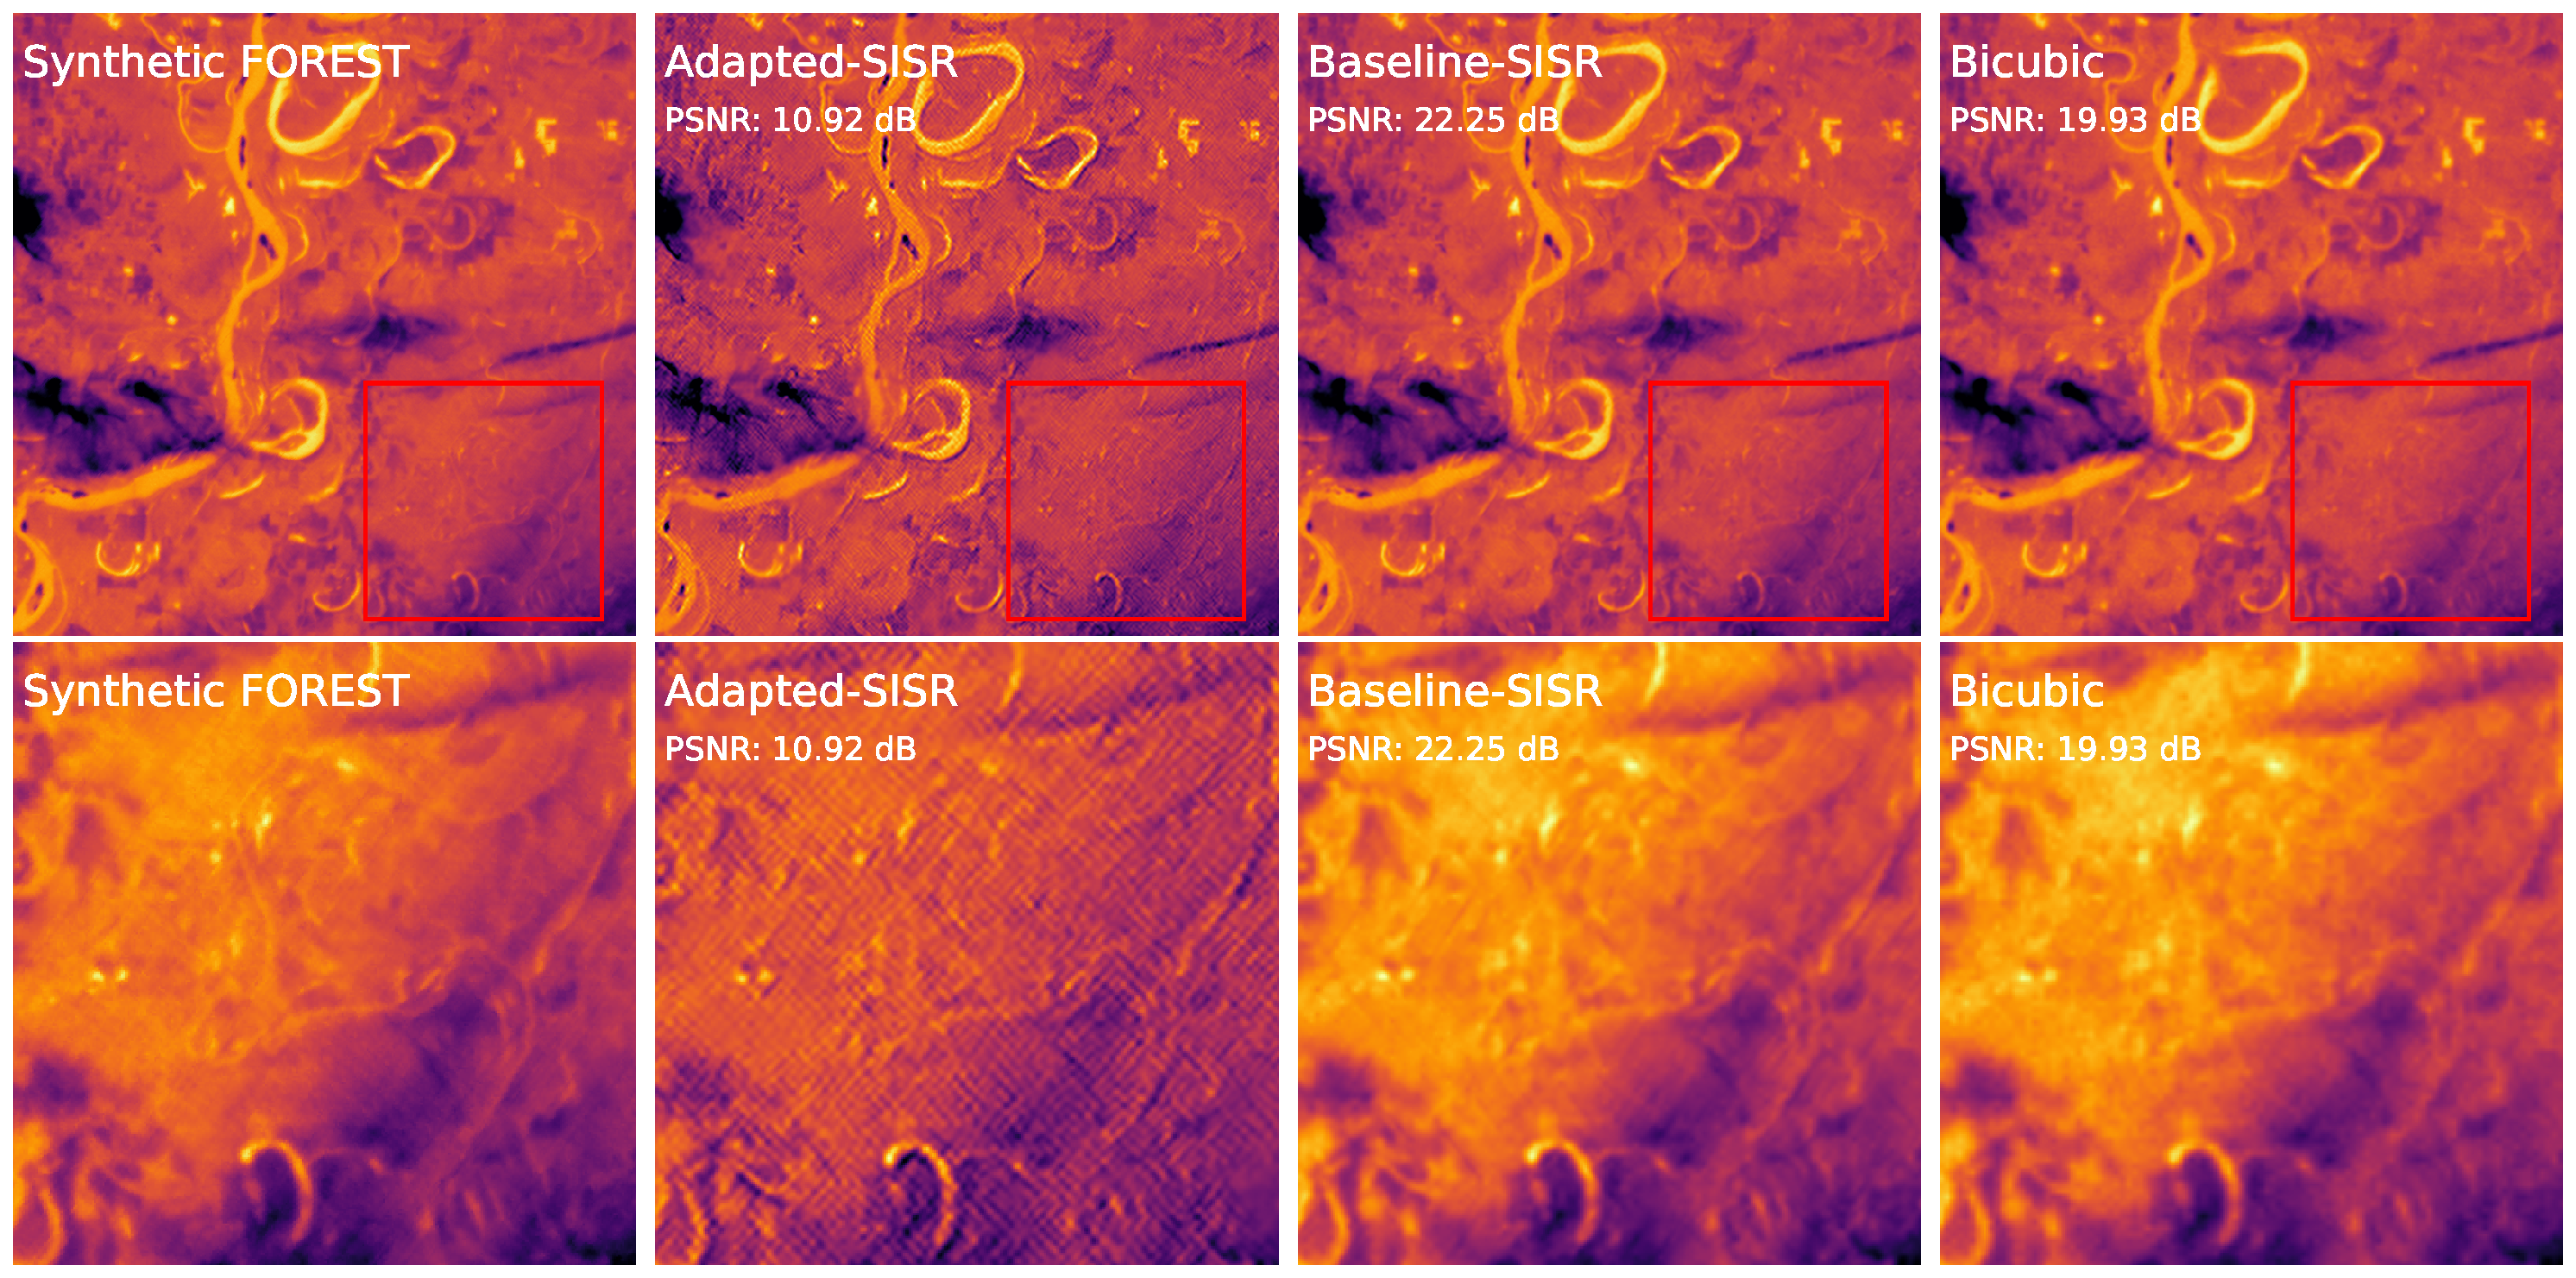
\includegraphics[scale=0.28]{Includes/5-target-prediction-with-domain-gap.pdf}
            \caption{Effects of using a model trained with on different domain than at inference time. 
                     When using an Synthetic FOREST image degraded with the baseline degradation model as an input, the model trained using real FOREST-2 data as the target domain generates several artifacts and underperforms severly in terms of PSNR. }
            \label{fig:5-target-prediction-with-domain-gap}
        \end{figure}

        In the frequency domain, the results  are shown in Fig. \ref{fig:5-target-prediction-with-domain-gap-fft}.  
        The adapted model adds amplification in the higher range of spatial frequency, related with noise and artifacts.
        The frequencies of interest are also amplified.
        This suggests that while the adapted model highlights edges and details, it also severely amplifies the noise and artifacts, resulting in a worse performance in terms of PSNR.
        % It is important to note that the amplification curve does not show a considerable difference with respect to the one in Fig. \ref{fig:5-target-amplification-statistics},
        % highlighting the fact that the frequency analysis is not suitable by itself to evaluate the performance of the SR model.

        \begin{figure}[H]
            \centering
            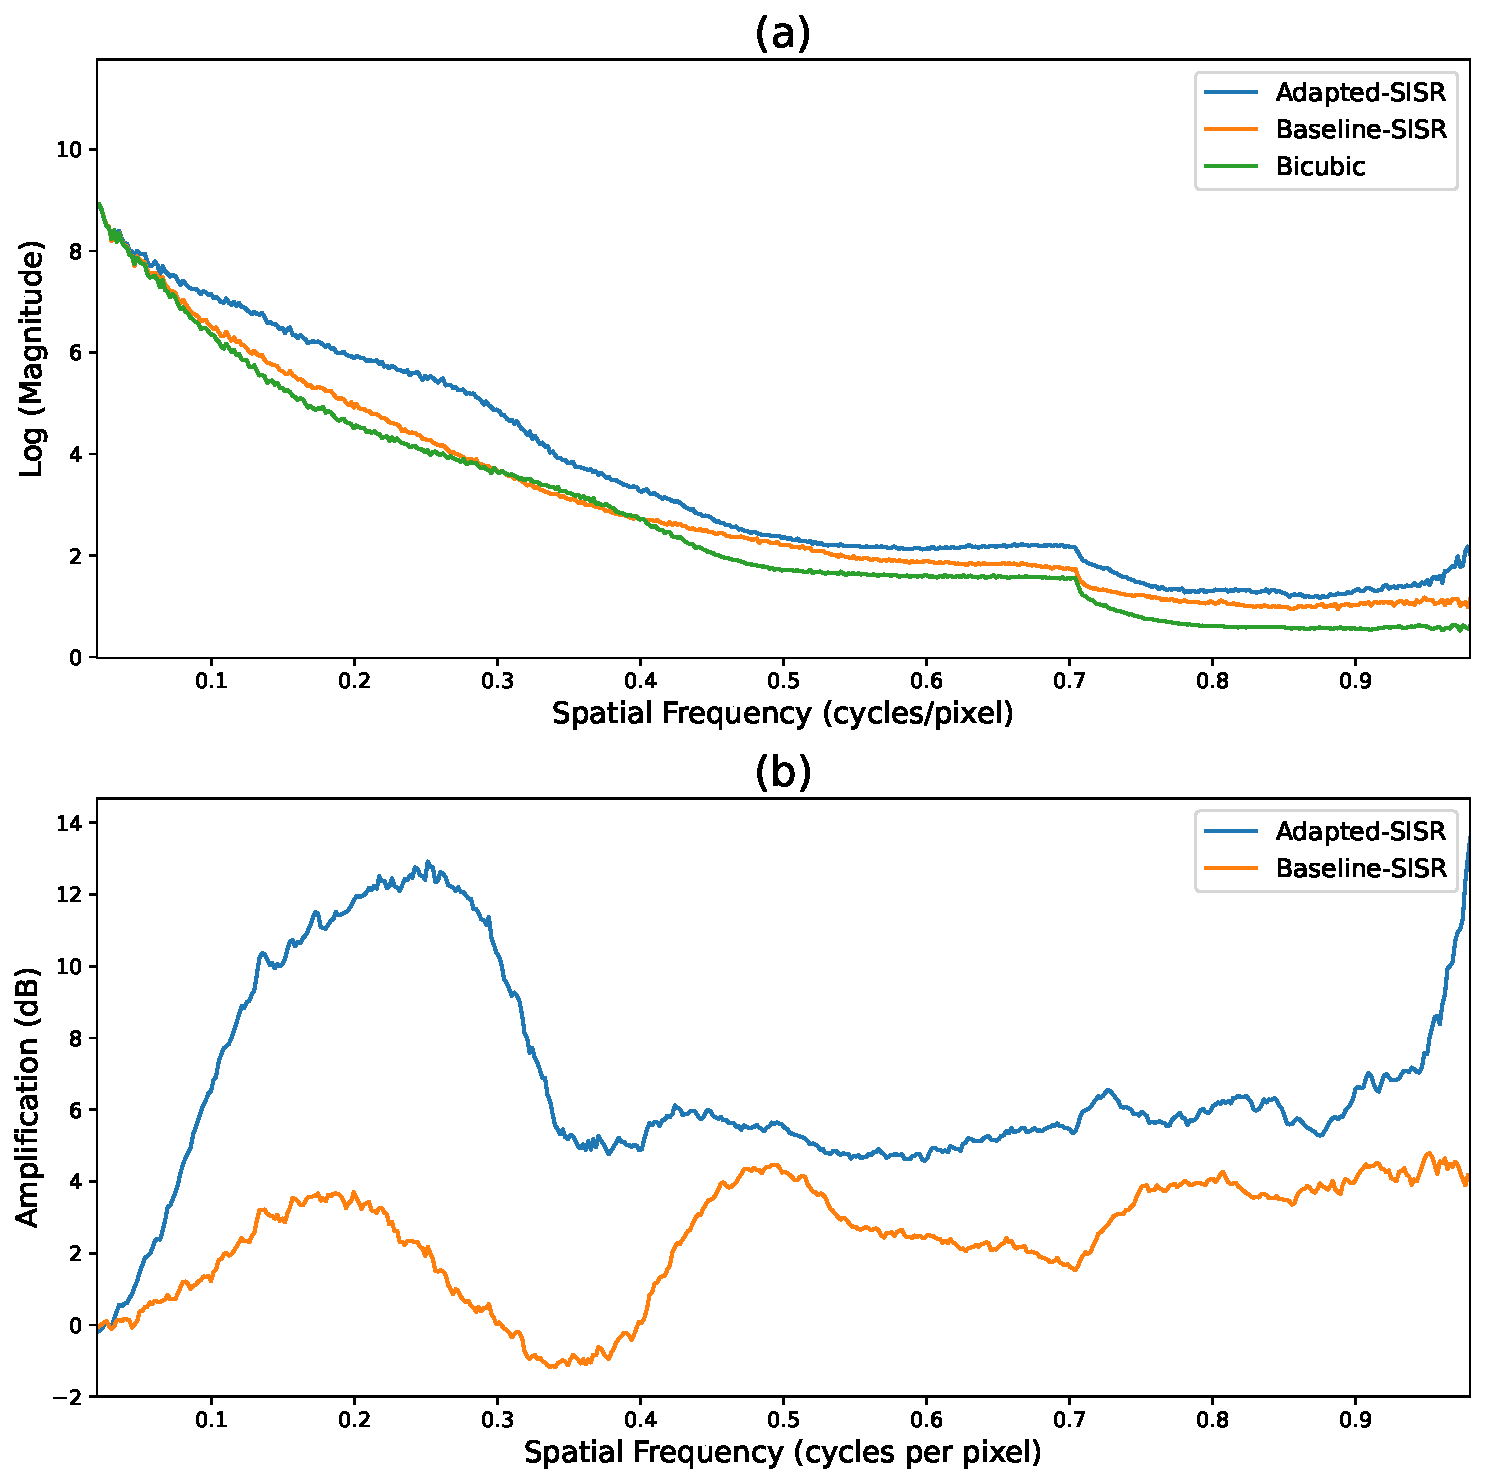
\includegraphics[scale=0.4]{Includes/5-target-prediction-with-domain-gap-fft.pdf}
            \caption{Effects of using a model trained with on different domain than at inference time. 
                     (a) shows the log magnitude of the radial average of the FFT for the SR images using different algorithms.
                     (b) shows the amplification with respect to bicubic interpolation.
                     }
            \label{fig:5-target-prediction-with-domain-gap-fft}
        \end{figure}


        The performance results in terms of different metrics are shown in Fig. \ref{fig:5-target-prediction-with-domain-gap-dataset}. 
        In the conditions described above, the adapted super resolution model underperforms severly in every considered metric.


        \begin{figure}[H]
            \centering
            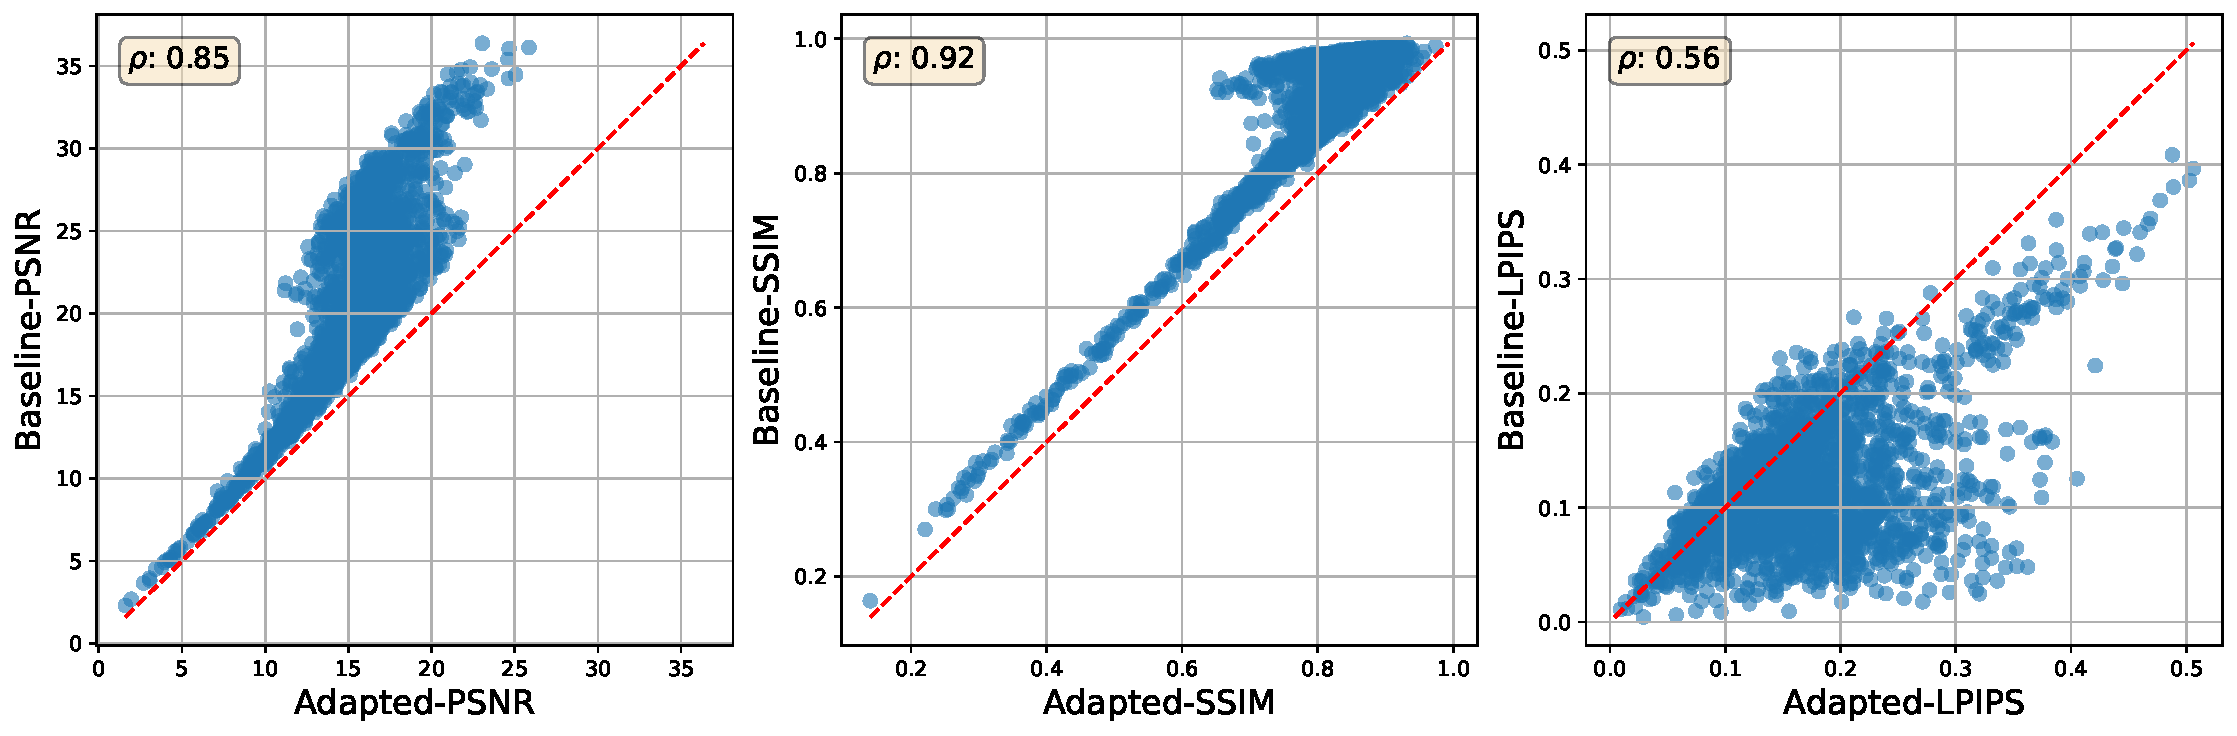
\includegraphics[scale=0.38]{Includes/5-target-prediction-with-domain-gap-dataset.pdf}
            \caption{Performance obtained by super resolving the degraded synthetic FOREST images using different super resolution models.}
            \label{fig:5-target-prediction-with-domain-gap-dataset}
        \end{figure}
        
        
    This demonstrates that while this approach is very good to bridge a domain gap, it is not robust at all to domain shifts. 
    This limitation is in sync with what is found in the literature, where GAN approaches are not able to generalize to arbitrary domains DASDASD.

    \subsection{Domain gap using non-references image quality assessment}

    As in the target domain the ground truth is not known due to the lack of a paired dataset, the performance of the SR model can not be evaluated using metrics like PSNR and SSIM.
    The image quality assessment metrics was done for $\mathcal{D}_{\text{SF}-\text{RF}}$ and $\mathcal{D}_{\text{SF}-\text{SF}}$, calculating the NIQE and BRISQUE scores of all the super resolved images from each validation dataset.
    
    The results are shown in Fig. \ref{fig:5-target-iqa-results}.
    For both metrics, a large gap is observed between the adapted model and the rest for dataset $\mathcal{D}_{\text{SF}-\text{RF}}$, suggesting that the adapted model is able to produce more natural images than the rest.
    This behaviour does not replicates when the input images come from $\mathcal{D}_{\text{SF}-\text{SF}}$.
    
    Moreover, for the adapted model, both metrics tend to get worse when the input images come from synthetic FOREST-2 images. The contrary happens for the rest of the models.
    This suggests that any SR model is able to produce more natural images only when the input images come from the same distribution as the target domain used in training.
    
    However, it is important to note that: 

    \begin{enumerate}
        \item The images used for training the NIQE and BRISQUE models are not remote sensing images, and therefore, the results may not be representative. This could be circumvented by training a NIQE/BRISQUE model using remote sensing images only.
        \item NIQE and BRISQUE are objective measures of image quality, not of physical consistency or image fidelity.
    \end{enumerate}

    While the comparison of results may help to understand the behaviour of the models, it is important to note that the results are not representative of the real world performance of the models. 

        \begin{figure}[H]
            \centering
            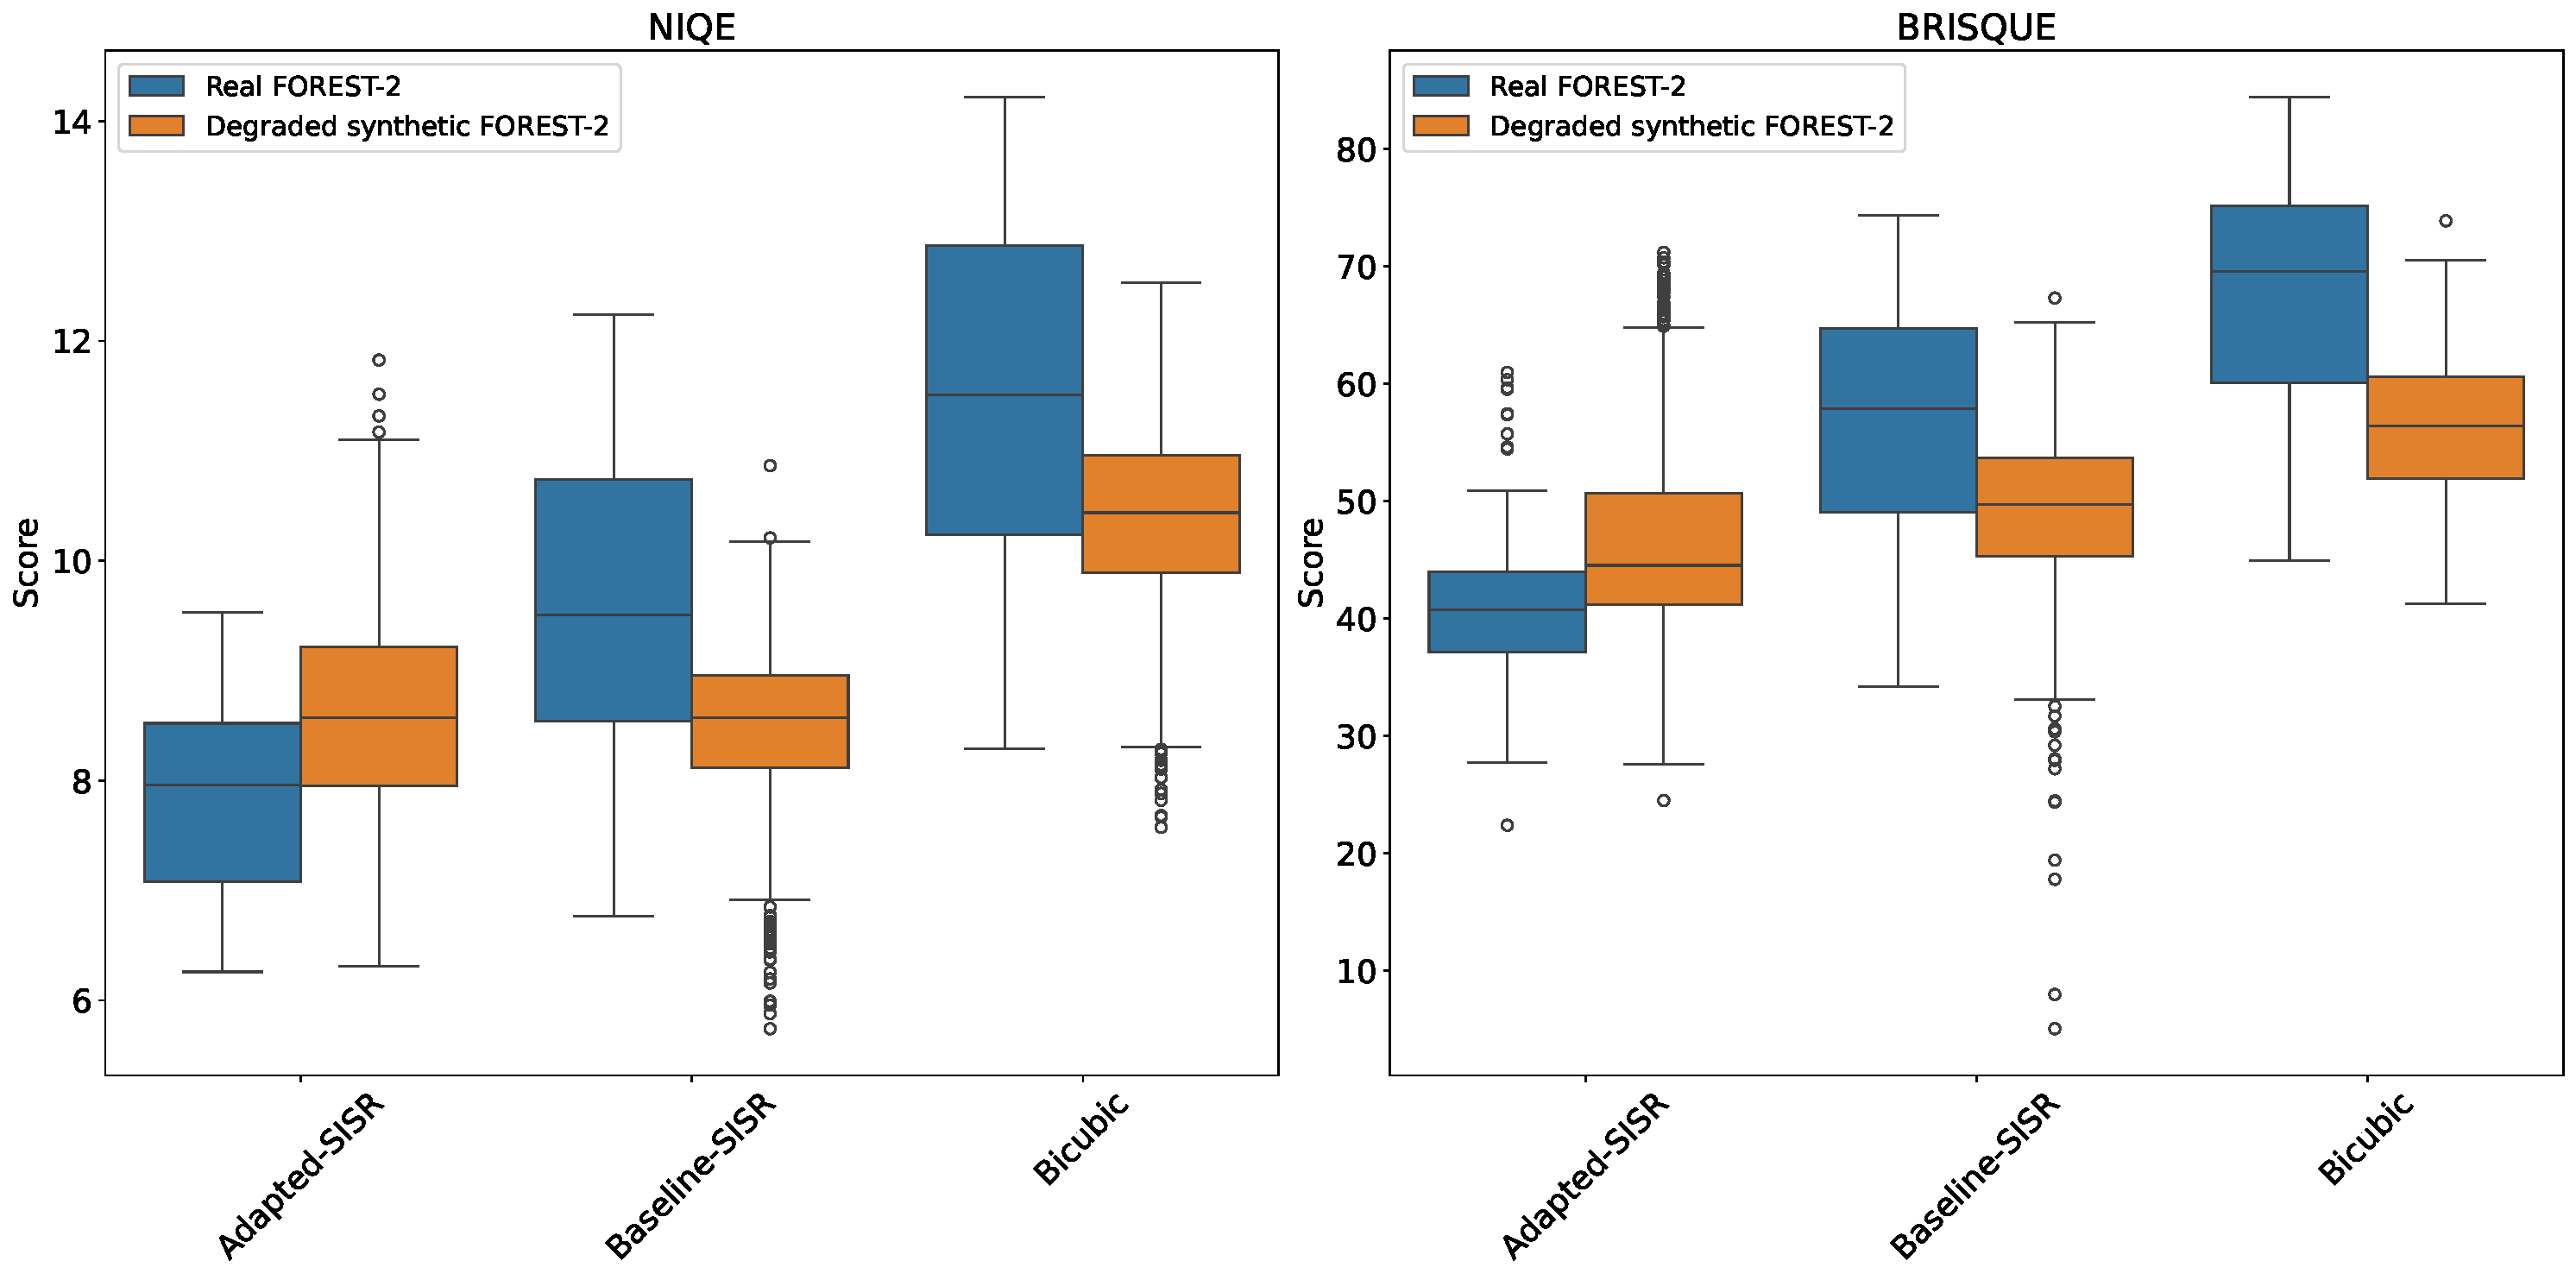
\includegraphics[scale=0.28]{Includes/5-target-iqa-results.pdf}
            \caption{Image quality assessment metrics for the different SR models using different datasets as input. 
                    In both metrics, the lower the score, the better the image quality.}
            \label{fig:5-target-iqa-results}
        \end{figure}


        

        
\newpage
    
\section{Conclusions and future work}

In this thesis, the feasibility of applying blind single-image super resolution algorithms to thermal remote sensing data in real world environments was studied with satisfactory results. The framework used is very flexible, requiring only two unpaired datasets with enough data. Additionally, one of the contributions of this work is the development of methods that may help in the assessment of performance without the need for paired data. While they are not sufficient to quantify the performance of the SR model, they are a good indicator of the quality of the results.

The work started , by introducing the fundamentals of remote sensing, the importance of thermal infrared data for land surface temperature estimation, and the dimensions of quality that they present.
Applications of LST products like wildfire management and urban heat studies require high spatial and temporal resolutions, which are not available in the current options. 
Because of different variables like payload capacity of the missions, sensor technology and the cost of the missions, there is a trade-off betweem spatial and temporal resolutions that is not possible to circumvent at the present day.
While Ororatech has a plan to improve the temporal resolution using swarms of small satellites like FOREST-2, the spatial resolution remains a challenging problem.

Super resolution techniques offer a promising solution, being SISR the most straightforward of them. As a supervised problem, they require a paired dataset of HR-LR images. This is not possible for FOREST-2, because HR images are not available.
To circumvent this issue, data from external missions with better resolution like ECOSTRESS was used to generate a syntheticly generated HR FOREST-2 dataset. ECOSTRESS is an ideal candidate for the task because of its spectral and spatial characteristics that match very well with FOREST-2.
An automated process for fetching the data from the NASA API,and process it was developed.

However, it is still not possible to obtain paired data, as the scenes from ECOSTRESS and FOREST-2 are different. Most of the literature in super resolution rely on downscaling the HR images using a gaussian kernel and adding white noise to generate the LR pairs required for training. 
In the results section, it was proved that this approach is not up to the task. The domain gap between the synthetically degraded and real images is too big , resulting in an SR model that is not able to generalize to FOREST-2 images, producing blurry images.

Blind super resolution techniques were explored as a solution. The availability of FOREST-2 data drived the decision of using a implicit modelling of the degradation process, through a GAN architecture for the degradation. A probabilistic degradation model was proposed for the task, as its well-constrained kernel and noise modules allow the training of an end-to-end pipeline of degradation + SR. Additionally, sampling from the degradation distribution allows to generate a wide variety of HR-LR pairs from only one HR image, which is very useful for the training of the SR model.

The degradation model adapted to FOREST-2 images and it's effects were studied by comparing them to a baseline gaussian + noise degradation. The results showed that this adapted model produces LR images that are blurrier, and consistently with more noise than the baseline, implying that FOREST-2 degradation model is more complex.
Its kernel module is not gaussian, and the noise has a big dependence on the content of the image, implying that the noise is not white. 
The LR images generated by the adapted degradation model are more challenging for SR than the baseline, as proven when applying bicubic upsampling to them and comparing them with the HR.  
The frequency domain analysis showed similar conclusions, where the adapted degradation model produced images a more narrow frequency response than the baseline.

Surprisingly enough, the result of super resolving LR images coming from the adapted degradation model and the baseline yielded very similar results. This means that the SR model, despite starting from very different LR images, was able to reconstruct the HR image with similar quality. This displays the power of the SR model, and the fact that it is being under-utilized when using bicubic downsampled LR images. Despite this, a "hard-limit" for the SR is observed and there seems to be a upper bound to the PSNR that the model is being able to obtain. The introduction of newer SISR methods or multi-spectral SR may be beneficial to overcome this limitation.

When comparing the results of the adapted SR model with the baseline on real FOREST-2 images, a lot more of detail and edges seem to be present, at a cost of a small increment in the overall noise. 
The images have stronger components in a range of frequencies, compared with bicubic upsampling, in the order of 6dB. Additionally, the frequencies match the ones lost during the degradation process, implying that the adapted SR model is able to recover the lost frequencies during the degradation process.
This phenomena can also be observed by analyzing the gradient magnitude of the images, where the adapted SR model produces images that tend to have bigger gradients, implying sharper edges. 
While the model was trained on thermal infrared data, it was proven robust to be used directly on LST products. This allows to improved the spatial resolution of LST images that were already processed from TIR data, without the need of reprocessing them.

However, the model is still very sensitive to the domain gap. 
When applying the adapted SR model to bicubic downsampled images, the results are catastrophic.
The edges of the images seem to be sharper but several artifacts appear, and the frequencies usually related to noise are dangerously amplified. 
In this case, the common situation is reversed, the estimated degradation kernel is more complex than the actual one, resulting in "over-amplification". This also highlights the difficulty of hand-picking the degradation model in classical dataset generation techniques, as it is very easy to be very optimistic or very pessimistic when choosing the amount of degradation.
The phenomena was also analyzed using non-referenced image quality assessment metrics, where the adapted SR model has significantly better score only when the input are real FOREST-2 images. Additionally, the adapted SR model was the only model that got worse scores when the input was bicubic downsampled images instead of real FOREST-2 images.
The sensitivity to differences between training and arbitrary inputs is a very relevant result, as it shows the limtations of the implicit modelling approaches. While they clearly help to bridge the domain gap, they are not able to generalize to an arbitrary input that is outside of the target domain.


Overall, the combination of probabilistic degradation modelling and SR yielded very promising results. It is a very flexible approach, in the sense that it only requires two sufficiently large datasets that  don't need to be paired. The latter is a very important advantage, as it is very difficult to obtain paired data in remote sensing, but unpaired data is abundant. The mentioned drawbacks of implicit modelling are not as relevant here, compared to other tasks, because the conditions of the missions (and their degradation models) are almost static. Unlike other domains like natural images, where the amount of possible cameras and sensors are almost infinite, the number of sensors and in a satellite remains the same and only the change of conditions because of time should be taken into account. This means that the degradation model can be trained on a very specific domain, and the LR input that will be used in the future will probably come from the same distribution.
Fortunately, the low difficulty of training models with this approach allows to have multiple SR models, one for each wanted target domain, with low effort.

Despite using unpaired data for training, the lack of a paired HR-LR dataset still poses a challenge. While the results are promising, it is not possible to quantify how good the adapted SR model in super resolving real FOREST-2 images compared to other methods due to the lack of a ground truth HR image. 
This also provokes a limitation in model training. Right now, the best model during training is chosen as the one that maximizes the PSNR on the source domain of the validation set (That means, taking the HR image, degrading it to LR, super resolving it and comparing to the HR). While this is not a bad criteria at all, it would be better to pick the one that maximizes the PSNR on the target domain ( directly upsampling the real FOREST-2 images), as it will be the relevant metric in a production environment. In order to do this, a paired dataset of at least 100 images of real FOREST-2 images paired with their HR counterparts is needed.

While the super resolution model is already being used in LST calculation pipelines of OroraTech, there is still room for improvement. Possible directions of future work will be discussed further:

\begin{itemize}
    \item The probabilistic degradation modelling assumes complete independence between the noise and kernel components. While it is a reasonable assumption, it may not be true in all cases.
    \item As explored in the implicit modelling section. The addition of a discriminator that distinguishes between the HR image and the super resolved real FOREST-2 images may improve the quality of the results even further by aligning their distributions without the need of them being paired.
    \item In the future, OroraTech will launch a swarm of small satellites called FOREST-2. They will have similar properties, but the degradation model may be different. When the data is available, investigating wheter a general model for all FOREST data products is possible or if each mission needs its own model will be interesting.
    \item While NIQE and BRISQUE may be helpful to assess the quality of the Super resolution without a reference, their corresponding models are trained on natural images. The development of NIQE/BRISQUE metrics trained on remote sensing data may be more suitable for the task.
    \item The introduction of newer SISR architectures, or the incorporation of information from other spectral bands to do MSSR as in \cite{myself2023} may be beneficial to overcome the "hard-limit" of the SR model. MISR is also very promising, but the difficulty to obtain multi-image data from FOREST-2 is a challenging limiation for its application.
    \item Because of how the frequency domain analysis is done, the value for one normalized spatial frequency is the average on every direction. This approach could be further developed to focus on specific directions, as the real degradation model is probably not isotropic.
\end{itemize}


\newpage

\pagestyle{empty}
\bibliographystyle{unsrt}
\bibliography{bibliography}


\end{document}


